

\documentclass[authoryear,3p,times,preprint,review,fleqn]{elsarticle}

% ------------------------
%    Packages used
% ------------------------

% \usepackage[paper=a4paper,top=1.5cm,left=1.2cm,right=0.8cm,
%     foot=1cm,bottom=1.5cm]{geometry}

\usepackage[utf8]{inputenc}    % utf8 support       %!!!!!!!!!!!!!!!!!!!!
\usepackage[T1]{fontenc} 
\usepackage{amsmath,amssymb, amsthm,mathtools,mathrsfs,stmaryrd,titletoc}


% bibtex 
\usepackage{natbib}
% biblatex
% \usepackage[hyperref=true,natbib=true,backref=true,style=authoryear-comp,giveninits=true,maxbibnames=9,maxcitenames=2,uniquelist=false,sortcites=none,doi=false,url=false,eprint=false,uniquename=false,dashed=false]{biblatex}
% \bibliography{mpm.bib,mpm_SS.bib}


%\usepackage{bm}% bold math
%\usepackage[scaled=0.92]{helvet}  % set Helvetica as the sans-serif font
%\renewcommand{\rmdefault}{ptm}    % set Times as the default text font
% need to install mtpro2
\let\Bbbk\relax
\usepackage[subscriptcorrection,slantedGreek,nofontinfo,mtphrd]{mtpro2}

\usepackage[retainorgcmds]{IEEEtrantools}
\usepackage[usenames]{color}
\usepackage{tabularx}
\usepackage{booktabs}
%\usepackage{psfrag}
%\usepackage{scalerel} % for large angle brackets <>, does not work
%\usepackage{cite}
%\usepackage[authoryear,sort,nonamebreak,sectionbib]{natbib} 
%\usepackage[authoryear,nonamebreak,sectionbib]{natbib} 
\usepackage[font=small,labelfont=md]{caption,subfig}
\usepackage{multirow}
\usepackage[T1]{fontenc} % typing french
%\usepackage{fancyhdr}
%\usepackage[english,hyperpageref]{backref}                         
\usepackage[bookmarks=true,colorlinks=true,linkcolor=blue,citecolor=red,backref=page]{hyperref}
\usepackage{makeidx}       % make index
\usepackage{float}         % make new float environment such as boxes (captioned)
\usepackage{listings}      % insert source code   
%\usepackage{bm}
\usepackage{algorithm}
\usepackage{algorithmicx}
\usepackage{algpseudocode}
\usepackage{tcolorbox}
\usepackage{mathtools}
%\usepackage[ruled,vlined]{algorithm2e}
%\sloppy
%\usepackage{authblk}



% nomenclature and glossaries for XFEM, CDM
\usepackage{nomencl}
\usepackage[acronym]{glossaries}

% the following packages just to improve the latex experience 
%\usepackage{silence} %
\usepackage{silence}
\WarningsOff
\usepackage{siunitx}
\usepackage[norefs,nocites,ignoreunlbld]{refcheck} % warning for unreferred figs/tables/equas
% search in the .log file for unused fig to detect figures not referred to in the text.
\usepackage[activate={true,nocompatibility},final,tracking=true,kerning=true,spacing=true,factor=1100,stretch=10,shrink=10]{microtype}
% activate={true,nocompatibility} - activate protrusion and expansion
% final - enable microtype; use "draft" to disable
% tracking=true, kerning=true, spacing=true - activate these techniques
% factor=1100 - add 10% to the protrusion amount (default is 1000)
% stretch=10, shrink=10 - reduce stretchability/shrinkability (default is 20/20)
%\usepackage{varioref}
\usepackage[capitalise]{cleveref} %Basically, cleveref must be loaded last.
% clever ref: instead of Fig.~\ref{d}, use \cref{d} or \Cref{d}  capitalise -> Figure 1
% \crefrange{eq1}{eq5}
\usepackage[textsize=tiny]{todonotes}
\usepackage{nicefrac} % type inline fractions: \nicefrac{1}{2}
\usepackage{setspace}
\usepackage{lineno}  % write numbers for lines
%\usepackage[mediumspace,mediumqspace,Grey,squaren]{SIunits}
\usepackage{totcount} % to count the total number of references and other things
\usepackage[figure,table]{totalcount}
\usepackage{blkarray, bigstrut} % write complicated matrices with borders, see http://mirror.lagoon.nc/pub/ctan/macros/latex/contrib/blkarray/blkarray.pdf
\usepackage{setspace}
\usepackage{tikz}
\usetikzlibrary{arrows,decorations.pathmorphing,decorations.pathreplacing,backgrounds,positioning,fit,matrix,math,shapes.misc}
\tikzset{cross/.style={cross out, draw=black, minimum size=2*(#1-\pgflinewidth), inner sep=0pt, outer sep=0pt}, cross/.default={1pt}}
\usepackage{wasysym}
\usepackage{gensymb} % for degree symbol

\usepackage{pgfplots}
 \pgfplotsset{compat=newest}
 %% the following commands are needed for some matlab2tikz features
 \usetikzlibrary{plotmarks}
 \usetikzlibrary{arrows.meta}
 \usepgfplotslibrary{patchplots}
 \usepackage{grffile}
\usepackage{pgf}
%\usepackage{underscore}
\usepackage[english]{babel}

%\makeatletter
\renewcommand\fs@ruled{\def\@fs@cfont{\bfseries}\let\@fs@capt\floatc@ruled
\def\@fs@pre{\hrule height 1.2pt depth0pt \kern2pt}%
%\def\@fs@post{\hrule height1.2pt depth0pt \kern2pt}%
\def\@fs@post{\kern2pt\hrule height 1.2pt depth0pt \kern2pt \relax}%
\def\@fs@mid{\kern2pt\hrule\kern2pt}%
\let\@fs@iftopcapt\iftrue}
\makeatother

% index generation
% see LATEX companion p 354
\newcommand{\bs}{\symbol{'134}}%print backslash
\newcommand{\Com}[1]{\texttt{\bs#1}%
\index{#1@\texttt{\bs#1}}}
\newcommand{\Prog}[1]{\texttt{#1}%
\index{#1@\texttt{#1} program }}

% shortcuts

% inner product <x,y>
\newcommand{\ipn}{\langle \cdot , \cdot \rangle}
\newcommand{\ip}[2]{\langle #1 , #2 \rangle}

% norm ||x||
\newcommand{\normn}{\left|\left| \cdot \right|\right|}
\newcommand{\norm}[1]{\left|\left|#1\right|\right|}
\newcommand{\meas}[1]{\left|#1\right|}

% McAuley brackets <x>
\newcommand{\mcauley}[1]{\langle #1 \rangle}

\newcommand{\x}{~$\times$~}
\newcommand{\fig}{Fig.~}
\newcommand{\eref}[1]{(\ref{eq:#1})}
\newcommand{\sref}[1]{\ref{section:#1}}
\newcommand{\fref}[1]{\ref{fig:#1}}
\newcommand{\tref}[1]{\ref{table:#1}}
%\newcommand{\eref}[1]{Eq.~(\ref{#1})}
%\newcommand{\erefs}[1]{Eqs.~(\ref{#1})}
%\newcommand{\fref}[1]{Fig.~\ref{#1}}
%\newcommand{\frefs}[1]{Figs.~\ref{#1}}
%\newcommand{\tref}[1]{Table~\ref{#1}}
\newcommand{\trefs}[1]{Tables~\ref{#1}}
%\newcommand{\sref}[1]{Section~\ref{#1}}
\newcommand{\srefs}[1]{Sections~\ref{#1}}
\newcommand{\crefs}[1]{Chapters~\ref{#1}}
\newcommand{\aref}[1]{Appendix~\ref{#1}}
\newcommand{\tsty}{\textstyle}
\newcommand{\dsty}{\displaystyle}
\newcommand{\D}{\displaystyle}
\newcommand{\arrow}{~$\rightarrow$~}
\newcommand{\otheta}{\overline \theta}
\newcommand{\mathG}{\mathcal{G}}

\newcommand{\mi}{_\mathrm{m}}
\newcommand{\ma}{_\mathrm{M}}

\newcommand{\Mi}{^\mathrm{m}}
\newcommand{\Ma}{^\mathrm{M}}

\newcommand{\dep}{_\mathrm{d}}
\newcommand{\ind}{_\mathrm{i}}

\newcommand{\di}{\mathrm{d}}

\newcommand{\defi}{\mathrel{\mathop:}=}

% abbreviations

\usepackage{xspace}
\newcommand{\eg}{\textit{e.g.}\xspace}
\newcommand{\ie}{\textit{i.e.},\xspace}
\newcommand{\etc}{\textit{etc.}\@\xspace}
\newcommand{\CF}{\textit{cf.}\,}     % i.e.
\newcommand{\cf}{\textit{cf.}\,}     % i.e.
\newcommand{\ETAL}{et. al.\@\xspace}
\newcommand{\etal}{et. al.\@\xspace}
\newcommand{\cmatrixb}{\left\{ \begin{matrix}}
\newcommand{\cmatrixe}{\end{matrix} \right\}}

% general vector/matrix commands:

\newcommand{\tvm}[1]{\textbf{#1}}
\newcommand{\tvms}[1]{$\boldsymbol{#1}$\ }
\newcommand{\vm}[1]{\mathbf{#1}}
\newcommand{\vms}[1]{\mathbf{#1}}
\newcommand{\bsym}[1]{\boldsymbol{#1}}

% vector/matrix for space coordinates 'x' and 'y'

\newcommand{\vx}{\mathbf{x}}
\newcommand{\vy}{\mathbf{y}}
\newcommand{\ve}[1]{\mathbf{e}_{#1}}
\newcommand{\bx}{\boldsymbol{x}}
\newcommand{\vxI}{\mathbf{x}_{I}}
\newcommand{\vj}[1]{\mathbf{#1}_{j}}
\newcommand{\xI}{x_{I}}
\newcommand{\yI}{y_{I}}
\newcommand{\hvx}{\hat{\mathbf{x}}}
\newcommand{\hx}{\hat{x}}
\newcommand{\hy}{\hat{y}}

\newcommand{\trans}{^\mathrm{T}}
\newcommand{\transi}{^\mathrm{-T}}
\newcommand{\el}{_\mathrm{e}}
\newcommand{\pl}{_\mathrm{p}}

\newcommand{\inte} [1]{\int_\Omega #1 d\Omega}
\newcommand{\intE}[1]{\int_{\Omega_0} #1 d\Omega_0}
\newcommand{\intg}[1]{\int_{\Gamma} #1 d\Gamma}
\newcommand{\intG}[1]{\int_{\Gamma_0} #1 d\Gamma_0}



%\newcommand{\T}{\underline{\vm{T}}}

% Shortcuts for making slides

\newcommand{\fontone}{\bfseries\Large}
\newcommand{\fonttwo}{\bfseries\large}
\newcommand{\fontonesc}{\scshape\Large}
\newcommand{\fonttwosc}{\scshape\large}
\newcommand{\fontthree}{\bfseries}
\newcommand{\bc}{\begin{center}}
\newcommand{\ec}{\end{center}}
\newcommand{\bitem}{\begin{itemize}}
\newcommand{\eitem}{\end{itemize}}

% ************************ MATH TYPE MACROS **************************
\newcommand{\mth}[1]{\mathit{#1}}      % print standard math italics
\newcommand{\boldsym}[1]{\mbox{\boldmath${#1}$}}
\newcommand{\vct}[1]{\boldsym{#1}}     % print vector
\newcommand{\fnc}[1]{\prno{#1}}        % print function i.e. sin ...
\newcommand{\mtx}[1]{\mathbf{#1}}      % print matrix
\newcommand{\msc}[1]{\mathcal{#1}}     % print script
\newcommand{\mss}[1]{\mathsf{#1}}      % print sans sarif
\newcommand{\tns}[1]{\boldsym{#1}}     % print tensor
\newcommand{\dbl}[1]{\mathbb{#1}}      % print sets letters like |R |C, etc...
%\newcommand{\Grad}{\stackrel{\rightharpoonup}{\boldsym{\nabla}}\!\!}
                                       % print gradient operator
\newcommand{\GradL}{\!\!\stackrel{\leftharpoonup}{\boldsym{\nabla}}}
                                       % print gradient operator
\newcommand{\Grad}{\boldsym{\nabla}}
                                       % print gradient operator
\newcommand{\Div}{\Grad\cdot}          % print divergnece operator
\newcommand{\DivL}{\cdot\GradL}        % print divergnece operator

\newcommand{\ljump}{\lbrack \! \lbrack } % print left jump oerator
\newcommand{\rjump}{\rbrack \! \rbrack } % print right jump oerator
                                         % derivative
\newcommand{\jump}[1]{\ljump {#1} \rjump} % jump operator
\newcommand{\derivv}[2]{ \frac{d^2 {#1} }{d {#2}$^2$ } }
\newcommand{\deriv}[2]{ \frac{d {#1} }{d {#2} } }   % partial derivivative
\newcommand{\pderiv}[2]{ \frac{\partial {#1} }{\partial {#2} } }
\newcommand{\testspc}{\mathcal{V}}
\newcommand{\trialspc}{\mathcal{S}}

\newcommand{\volint}[1]{\int_{\Omega}\,{#1}\,dV} % integrals
\newcommand{\bndint}[2]{\int_{#1}\,{#2}\,dS}

\newcommand{\beq}{\begin{equation}}
\newcommand{\eeq}{\end{equation}}
\newcommand{\beqa}{\begin{eqnarray}}
\newcommand{\eeqa}{\end{eqnarray}}

%--My own definitions--

\newcommand{\reals}{{\mathbb R}}
\newcommand{\dof}{\emph{dof}}
\newcommand{\dofs}{\emph{dofs}}
\newcommand{\bfalfi}{\mbox{\boldmath$\alpha$\unboldmath$_i$}}
\newcommand{\bfalfj}{\mbox{\boldmath$\alpha$\unboldmath$_j$}}
\newcommand{\remark}[2]{\vspace{0.1cm}
\noindent {\bf Remark #1:}  {#2}  \vspace{0.1cm}}
\newcommand{\invisible}[1]{}
\newcommand{\bgl}[1]{\mbox{\boldmath$#1$\unboldmath}}
\newcommand{\parti}[2]{\frac{\partial #1}{\partial #2}}

% X-FEM related
\newcommand{\xfemlong}{\textit{eXtended Finite Element Method}\,}     % extend..
\newcommand{\xfem}{\textit{X-FEM}\,}     % x-fem

% ********************** VERBATIM AND IGNORE *************************
\newcommand{\bv}{\begin{verbatim}}
\newcommand{\V}{\verb}                  % EX: \V=-d{#@~}= Expr must
                                        % fit on a line

% ************************ FIGURE COMMANDS ***************************
\newcommand{\testpix}[1]{\fbox{\begin{minipage}[c]{\textwidth}
                      #1 \end{minipage} }}

%\ifpdf
% \newcommand{\putfig}[2]{\includegraphics[scale=#2]{#1.pdf}}
%\else
% \newcommand{\putfig}[2]{\includegraphics[scale=#2]{#1.eps}}
%\fi

\newcommand{\putpstex}[1]{\includegraphics{#1.pstex_t}}
% END FIGURE COMMANDS


 % write numbers for lines
 % comment out for final pdf
%\linenumbers

% cleverref package
\crefname{figure}{Fig.}{Figs.}
\crefname{equation}{Equation}{Equations}

% todonotes on the left margin
\reversemarginpar
%\setlength{\oddsidemargin}{3mm}
%\setlength{\evensidemargin}{-3mm}
%\setlength{\textwidth}{160mm}
%\setlength{\textheight}{220mm}


\renewcommand*{\backref}[1]{}
\renewcommand*{\backrefalt}[4]{[{%
    \ifcase #1 %
          \or Cited on page~#2%
          \else Cited on pages #2%
    \fi%
    }]}
    
% -------------------------
%     Header and footer
% -------------------------

% \pagestyle{fancyplain}
% %\addtolength{\headwidth}{\marginparsep}
% %\addtolength{\headwidth}{\marginparwidth}
% %\renewcommand{\chaptermark}[1]{\markboth{#1}{}}
% \renewcommand{\sectionmark}[1]{\markright{\ #1}}
% \lhead[\fancyplain{}{\bfseries\thepage}]{\fancyplain{}{\bfseries Sec. \thesection}}
% \chead[\fancyplain{}{\bfseries\leftmark}]{\fancyplain{}{\bfseries\rightmark}}
% \rhead[\fancyplain{}] {\fancyplain{}{\bfseries\thepage}} 
% \cfoot{}

%\floatstyle{ruled}
%\newfloat{Fbox}{thp}{lop}[chapter]
%\floatname{Fbox}{Box}
%
%\theoremstyle{remark}                                                                                                       
%\newtheorem{thm}{Theorem}[chapter]                                                                                          
%\newtheorem{rmk}[thm]{Remark}    


%% code listing

\lstloadlanguages{C++,Matlab,Python}
\definecolor{mygreen}{rgb}{0,0.6,0}
\definecolor{darkgray}{rgb}{0.95,0.95,0.95}
\lstset{backgroundcolor=\color{darkgray},
  basicstyle=\color{red}\ttfamily,
  keywordstyle=\color{blue}\bfseries
}

\lstdefinestyle{C++}
{
 basicstyle=\footnotesize, numbers=none, numberstyle=\tiny,%
 showstringspaces=false, language=C++, escapechar=|,frame=tb,
 commentstyle=\color{mygreen}
}


\lstdefinestyle{python}
{
 basicstyle=\scriptsize, numbers=left, numberstyle=\tiny,%
 showstringspaces=false, language=Python, escapechar=|,frame=tb,%
 commentstyle=\color{mygreen},
 morekeywords={inner, Function, TrialFunction, TestFunction, solve, FunctionSpace,VectorFunctionSpace,grad,
 LinearVariationalProblem, LinearVariationalSolver, dx,UnitSquareMesh, lhs, rhs, sym, method, region, dimension,run, solid, ulmpm, tlmpm,linear,cylinder,block,material,fix, group,set_dt,dump,run_time,NULL,initial_velocity_particles,sphere,damage_johnson_cook,shock,johnson_cook,velocity_nodes,x,y,z,T,vx,eos,strength,damage,s11}
}


\newtcolorbox[auto counter,crefname={Box}{Boxes}]{MyBox}[2][]{%
  colback=gray!5!white,colframe=red!75!black,fonttitle=\bfseries,before skip=20pt plus
  2pt,after skip=20pt,
  title=Box~\thetcbcounter: #2, #1}

\lstdefinestyle{commentstyle}{color=\color{green}}

\newcommand{\bfsigma}{\boldsymbol{\sigma}}
\newcommand{\bfepsilon}{\boldsymbol{\epsilon}}
\newcommand{\bfu}{\boldsymbol{u}}
\newcommand{\bfx}{\boldsymbol{x}}
\newcommand{\bfphi}{\boldsymbol{\phi}}
\newcommand{\bftheta}{\boldsymbol{\theta}}
\newcommand{\te}{\text{e}}
\newcommand{\td}{\text{d}}
\newcommand{\tp}{\text{p}}
\newcommand{\etc}{etc.\@\xspace}
%-----------------------------------------------------------------------
\newcommand{\tty}[1]{\textnormal{\texttt{#1}}}
\newcommand{\sym}[1]{\textnormal{\textit{#1}}}


\lstloadlanguages{C++,Matlab,Python}
\definecolor{mygreen}{rgb}{0,0.6,0}
\definecolor{darkgray}{rgb}{0.95,0.95,0.95}
\lstset{backgroundcolor=\color{darkgray},
  basicstyle=\color{red}\ttfamily,
  keywordstyle=\color{blue}\bfseries
}

\lstdefinelanguage{Sage}{%
    language     = Python,
   morekeywords={var, latex,  view, show, diff, integral, simplify, simplify_full}
}



\lstdefinestyle{C++}
{
 basicstyle=\footnotesize, numbers=none, numberstyle=\tiny,%
 showstringspaces=false, language=C++, escapechar=|,frame=tb,
 commentstyle=\color{mygreen}
}

\lstdefinestyle{C-numbered}
{
 basicstyle=\footnotesize, numbers=left, numberstyle=\tiny,%
 showstringspaces=false, language=C++, escapechar=|,frame=tb,
 commentstyle=\color{mygreen}
}

\lstdefinestyle{matlab}
{
 basicstyle=\footnotesize, numbers=left, numberstyle=\tiny,%
 showstringspaces=false, language=Matlab, escapechar=|,frame=tb,%
 commentstyle=\color{mygreen},
 morekeywords={cell, ones, repmat, intersect, unique}
}

\lstdefinestyle{latex}
{
 basicstyle=\footnotesize, numbers=left, numberstyle=\tiny,%
 showstringspaces=false, language=[LaTeX]TeX, escapechar=|,frame=tb,%
 commentstyle=\color{mygreen},
 morekeywords={cell, ones, repmat, intersect, unique,includegraphics,input,toprule,midrule,bottomrule,colorbox,table,tabularx,setlength,subfloat,figure,width}
}

\lstnewenvironment{snippet}[1][]
{
 \lstset{style=python, xleftmargin=5mm, gobble=4, #1}
}
{}

\lstnewenvironment{snippetlatex}[1][]
{
 \lstset{style=latex, xleftmargin=5mm, gobble=4, #1,tabsize=3}
}
{}

\lstnewenvironment{code-sage}[1][]%
{
   \noindent
   \minipage{\linewidth}
   \vspace{0.5\baselineskip}
  \lstset{style=Sage, xleftmargin=5mm, gobble=4, #1}
}
{\endminipage}

%%

\newcolumntype{C}{>{\centering\arraybackslash}X}
\newcolumntype{b}{X}
\newcolumntype{s}{>{\hsize=0.5\hsize}X}
\newcolumntype{L}{>{\raggedright\arraybackslash}X} 
\newcolumntype{R}{>{\raggedleft\arraybackslash}X} 

\flushbottom

\definecolor{Sun}{rgb}{0.164,0.126,0.322}
\definecolor{Green}{rgb}{0,0.300,0.300}
\definecolor{Red}{rgb}{0.4,0,0}
\definecolor{Grey}{RGB}{105,105,105}
\definecolor{White}{rgb}{1,1,1}

%\newcommand\Algphase[1]{%
%   \vspace*{-.7\baselineskip}\Statex\hspace*{\dimexpr-\algorithmicindent-2pt\relax}%\rule{\textwidth}{0.4pt}%
%      \Statex\hspace*{-\algorithmicindent}\textbf{#1}%
%      \vspace*{-.7\baselineskip}\Statex\hspace*{\dimexpr-\algorithmicindent-2pt\relax}%\rule{\textwidth}{0.4pt}%
%}

% for blocks in Algorithm
\algblockdefx{Start}{End}[1]{\textbf{#1}}{\textbf{end}}

%without this, xelatex would not work with fontspec
\DeclareTextCommand{\nobreakspace}{T1}{\leavevmode\nobreak\ }

%%% vertical rules in cyan color
%\makeatletter
%\renewcommand{\algocf@Vline}[1]{%     no vskip in between boxes but a strut to separate them, 
%  \strut\par\nointerlineskip% then interblock space stay the same whatever is inside it
%  \algocf@push{\skiprule}%        move to the right before the vertical rule
%  \hbox{\bgroup\color{cyan}\vrule\egroup%
%    \vtop{\algocf@push{\skiptext}%move the right after the rule
%      \vtop{\algocf@addskiptotal #1}\bgroup\color{cyan}\Hlne\egroup}}\vskip\skiphlne% inside the block
%  \algocf@pop{\skiprule}%\algocf@subskiptotal% restore indentation
%  \nointerlineskip}% no vskip after


\newcommand{\latex}{\LaTeX\xspace}
\numberwithin{equation}{section}

\graphicspath{{./figures/}} 

\newcommand\Lang[1]{\textsc{#1}}

\theoremstyle{remark}
%\newtheorem{thm}{Theorem}[section]
%\newtheorem{rmk}[thm]{Remark}
\newtheorem{rmk}{Remark}

% total number of references
%1. bibtex

% total number of references
\newtotcounter{citenum}
\def\oldcite{}
\let\oldcite=\bibcite
\def\bibcite{\stepcounter{citenum}\oldcite}



%\journal{Advances in Engineering Software}
%\journal{International Journal for Numerical Method in Engineering}

\begin{document}

%\newcommand\barbelow[1]{\stackunder[1.2pt]{$#1$}{\rule{.8ex}{.075ex}}}

\begin{frontmatter}



%\title{Modeling crack propagation of concrete gravity dams with the phase-field regularized cohesive zone model}
\title{\textbf{How to effortlessly write a high quality scientific paper in the field of computational engineering and sciences }}

%\tnotetext[label1]{Dedicate to }

% use optional labels to link authors explicitly to addresses:
% \author[label1,label2]{}
% \address[label1]{}
% \address[label2]{}

\author[1]{Vinh Phu Nguyen\corref{cor1}}
 \ead{phu.nguyen@monash.edu}
\author[2]{Stephane Bordas}
\author[3]{Alban de Vaucorbeil}

\cortext[cor1]{Corresponding Author}

\address[1]{Department of Civil Engineering, Monash University, Clayton 3800, VIC, Australia}
\address[2]{Institute of Computational Engineering, University of Luxembourg, Faculty of Sciences Communication and Technology, Luxembourg}
\address[3]{Institute for Frontier Materials, Deakin University, Geelong, VIC, 3216, Australia}
%\maketitle


%\pagestyle{fancyplain}
%\pagenumbering{arabic}

\begin{abstract}
Starting with a working good research idea, this paper outlines a process that helps us to have a nearly complete paper when the last analysis task is finished.  The key ideas of this process are: (1) writing should start early in the research project, (2) research and writing are carried out simultaneously, (3) best tools for writing should be used.   Due to our personal preferences, the discussion is confined to \LaTeX\ based typesetting. The process seems working well as it has helped us writing thousands of pages without feeling a paint. We hope it works for you too. 

\end{abstract}

% *********************************************************************************************************

\begin{keyword}
 \LaTeX; scientific writing; .
\end{keyword}


\end{frontmatter}

\tableofcontents

%%%%%%%%%%%%%%%%%%%%%%%%%%%%%%%
\section{Introduction}

\showthe\textwidth % => width of the pdf, see in log file, is 468 pt. use it in plot.py for great plots.

Publishing original research in a peer-reviewed  journal is an important milestone for a scientist. It is an important parameter to assess academic achievements. 
However, technical and language barriers may prevent many enthusiasts from ever publishing. To help ease the writing process, books and articles giving advice on how to write scientific papers have been written \citep{day1998write,ashby2000write,plaxco2010art}. The value of writing well should not be underestimated: writing well leverages your work.

Building on the advice found in the literature and our total 20 years of experiences, this brief paper gives guidance in writing a paper about your research. Different from existing related works, see e.g. \cite{day1998write,ashby2000write}, we focus on the tools or softwares that ease our writing process. Due to our background in computational mechanics -- a sub-branch of computational engineering and sciences-- we have used, as a model, a typical computational mechanics project: one develops a new model, implements it in a code, and carries out simulations using that code to demonstrate the performance of the model. 

In \cref{sec:tools}, our favorite softwares are presented. These softwares are mostly open source and cross platform. \cref{sec:writing-tips} provides actionable suggestions on how to structure your paper, avoid common mistakes.  Particularly, we present an iterative writing process that is intertwined with your research.
As we use \LaTeX, a high-quality free typesetting system which is the de facto standard for the publication of scientific documents for hard sciences (see \cref{table:latex}), some \LaTeX\ related suggestions on how to prepare high-quality vector images, good-looking tables, tweaks for two-column format papers are provided (see \cref{sec:latex}). 

\begin{table}[h!]
      \centering
      \caption{Summary statistics of the use of \LaTeX\ in science disciplines (\% of submitted papers) taken from \url{https://www.the-scientist.com/uncategorized/dont-format-manuscripts-44040}.}
      \setlength\fboxsep{0pt}
      \vskip-\topsep%
      \smallskip%
      \renewcommand\arraystretch{1.4}
      \colorbox{darkgray}{%
      \begin{tabularx}{0.5\textwidth}{ll}
      \toprule
       Disciplines & \LaTeX\ rate \\
      \midrule
       Mathematics & 96.9\% \\
       Statistic and Probability & 89.1\% \\
       Physics & 74.0\%\\
       Computer Sciences & 45.8\%\\
       Engineering & 1.0\%\\
       \bottomrule
       \end{tabularx}%
      }
      \label{table:latex}
      \end{table}

With the pressure to “publish” (or perish), it is increasingly difficult for students to resist the temptation to submit a “large” number of papers during their PhD. Some of these might not be ready for submission yet. \cref{sec:submission} presents some considerations regarding this issue.


We have an admission: there is no single, correct way to write.  Our goal was not to convince you that we have found the one true way, but instead simply to get people thinking, talking and sharing about writing. 

It is obvious that, no matter how good you are as a writer, a bad research idea will not result in a good paper. Therefore, we  assume that you have had a  sound research idea. This paper outlines a process that helps us to have a nearly complete paper when the last analysis task is finished.  

The \LaTeX\ source of this paper and various \texttt{Python} scripts used to prepare good images can be found at the github account of the first author: \url{https://github.com/vinhphunguyen/how-to-write-a-paper}.



%%%%%%%%%%%%%%%%%%%%%%%%%%%%%%%
\section{Tools}\label{sec:tools}

It is obvious that using a right tool for any task is half way to success. And writing is no exception. Our favorite tools for writting papers are the following:

\begin{itemize}
\item \LaTeX:  a high-quality free typesetting system; it includes features designed for the production of technical and scientific documentation. It is the de facto standard for the communication and publication of scientific documents; 
\item \texttt{BibDesk}: an open-source reference management software package for macOS, used to manage bibliographies and references when writing essays and articles. It is primarily a BibTeX front-end for use with \LaTeX;
\item \texttt{JabRef}:  an open-source and cross-platform reference management software package. Its use is similar to BibDesk. It is primarily a BibTeX front-end for use with \LaTeX. One great feature that we like: it fetches bib entries automatically when given a DOI;
\item \texttt{Skim}: is an open-source PDF reader for macOS.
\item \texttt{Adobe Illustrator}: an industry-standard vector graphics software to create high quality drawings;
\item \texttt{Inkscape}: a free and open-source vector graphics editor available for Linux, macOS, and Windows;
\item \texttt{Matplotlib}: is a Python 2D plotting library which produces publication quality figures in a variety of hardcopy formats. It can be used in Python scripts;
\item \texttt{Dropbox}: on-going papers are stored in \texttt{Dropbox} so that we can access them from multiple devices;
\item \texttt{Git}: is a distributed version-control system for tracking changes in source code during software development.
\item \texttt{GitHub} or \texttt{Gitlab}: online platforms that offer hosting for software development version control using Git. They offer both public and private (preferred for research papers) repositories. When using Git, they make access from multiple devices and parallel collaboration easy.
\end{itemize}

The flowchart for the generation of a paper is as follows. \LaTeX~ is used to typeset the paper. The references used in the paper are stored in a \texttt{.bib} file automatically generated and managed by \texttt{BibDesk} or \texttt{JabRef}. Sketches used in the paper are drawn using \texttt{Adobe Illustrator} or \texttt{Inkscape} and graphs are created using \texttt{Matplotlib}. Sketches and graphs are saved as pdf files and thus of very high quality, see \cref{sec:figs}. Also, sketches and graphs could be generated such a way that the font used for embedded text is the same as that of your document.

To keep track of the changes in the code, figures, and even research data, \texttt{Git} is used. For collaborative writings, the git repository is hosted in either \texttt{Github} or \texttt{Gitlab}. They offer access to free private repositories that are very useful. This is because every co-author of the paper can work on the same paper simultaneously. They can also use their own favorite \LaTeX\ editor (which is most often also their own coding editor). We find this is better than \texttt{Overleaf} at \url{https://www.overleaf.com}.



% \begin{rmk}
% Note that \texttt{Bibdesk} is only available for mac OS. One can use \texttt{Zotero} or \texttt{Mendeley} for Windows and Linux computers. Alternatives to the quite pricey  \texttt{Adobe Illustrator} are \texttt{GIMP} or \texttt{Inkscape}.
% \end{rmk}

\begin{rmk}\label{rm:a}
Without going in to the debate of which is the best editor, we use \texttt{Sublime Text}. This is
because it can be used for both writing \LaTeX\ documents and coding. Furthermore, it can render equations in real time, see  \cref{fig:sublime-text}, which is quite handy. Two way sync between \texttt{Skim} and \texttt{Sublime Text} is super convenient. However, \texttt{Sublime Text} is proprietary. If you prefer open-sourced softwares, look into \texttt{Vim} and \texttt{Emacs}. Coupled with the \texttt{AucTex} package, \texttt{Emacs} can recognize \LaTeX\ code and compile it easily. For viewing the results, we like to use \texttt{Sumatra PDF} for Windows and \texttt{evince} for Linux.

\begin{figure}[h!]
  \centering 
   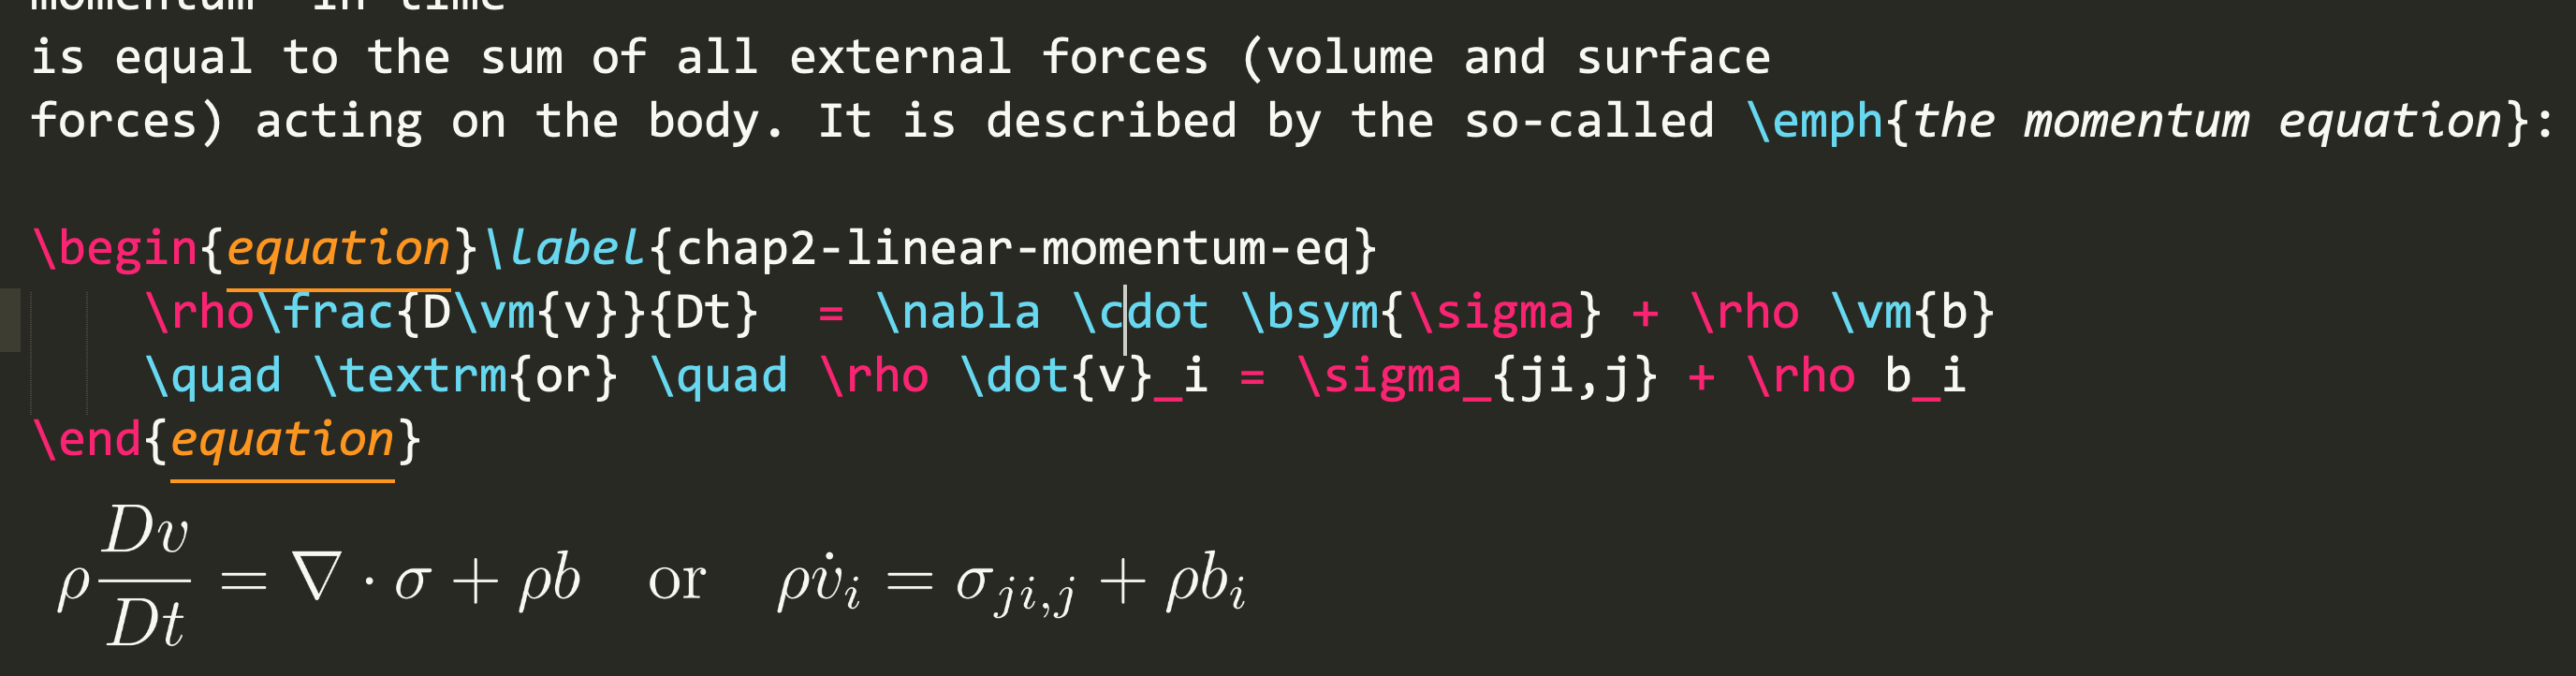
\includegraphics[width=0.65\textwidth]{sublime-text}
   \caption{\texttt{Sublime Text} can render equations in real time.}
\label{fig:sublime-text}
\end{figure}
\end{rmk}


%%%%%%%%%%%%%%%%%%%%%%%%%%%%%%%
\section{Writing tips}\label{sec:writing-tips}

\cref{sec:guidelines}
\cref{sec:writing-process}
\cref{structure}
\cref{sec:mistakes}

\url{https://www.youtube.com/watch?v=VK51E3gHENc}.

%--------------------------------------
\subsection{General guidelines}\label{sec:guidelines}

The following general guidelines are nothing new but they are worthy being repeated:

\begin{enumerate}
\item To inform not to impress;
\item Aim for clarity and readability;
\item Contributions must be clearly stated;
\item Each paragraph conveys a single idea or message only;
\item Avoid jargon;%  Writing a paper is not a race for complexity. You should make it as simple as possible for a neophyte reader to understand;
\item Aim for reproducibility;
\item Minimize chances for reviewers to raise issues;
\end{enumerate}

The main contributions of your paper must be clearly stated after a brief review of the literature: in which way your work differs from the existing literature. Be precise, as this is where the reviewers will try to find problems with your work. Their goal is to identify whether your work is novel or not. If it is not immediately clear from the Abstract and Introduction you risk being unconvincing. 

Do not be afraid of writing short paragraphs, even two-sentence ones. Each paragraph conveys only a single idea or message. Use simple sentences. Try to revise your writing to keep only those words that are necessary. For example, `because' is enough instead of the wordy `due to the fact that' (see \cref{tab:mistakes}).

Avoid jargon.  Writing a paper is not a race for complexity. You should make it as simple as possible for a neophyte reader to understand.
The advice is try to avoid jargon in the abstract and introduction as much as possible so that your paper is more accessible to a wide range of audience. However, it is not easy to do so as knowing the name of something doesn’t mean you understand it, according to Richard Feynman -- the well known American theoretical physicist.

Reproducibility is a big issue in scientific research nowadays. However, we just confine yourselves here to the situation where a published simulation result is genuinely correct but impossible to reproduce by people other than the authors. The world would be a better place if all authors are more thoughtful when reporting their results: all information needed to make that particular simulation work should be provided. Particularly, nontrivial parameters.

You can save time for both you -- the authors -- and the reviewers by not making them guess. For example, if you do not do large deformation simulations, make it clear and justify that choice. If you have used a particular value for one numerical parameter, explain your choice. If reviewers have to guess your choices, they will comment on that. This increases the chances for your paper to be rejected, or needing corrections.




%%%%%%%%%%%%%%%%%%%%%%%%%%%%%%%
\subsection{How to structure your paper}\label{structure}


An excellent article on how to structure a scientific paper can be found at \url{https://www.nature.com/scitable/topicpage/scientific-papers-13815490/}. However, they are just general guidelines. A good strategy for getting started is to study how others have structured their papers. Select a couple of papers that you enjoy and understand and study how they are organized. You will learn a lot from copying these papers. Our favorite author is Ted Belytschko.

 We will not repeat that herein. Instead, we elaborate some of the arguments such as a complex section should have a global paragraph before going into its subsection (\cref{sec:global-para}), (\cref{sec:introduction-part}), and 
what the conclusion section (\cref{sec:conclusion-part}) should include.  

\subsubsection{Global paragraph for long sections}\label{sec:global-para}

For paragraphs that are quite complex it is a good idea to write a global paragraph between the heading of a section and the heading of its first subsection. Remember to prepare your readers for the structure ahead at all levels. See \cref{fig:section} for an example. 


\begin{figure}[!h]
  \centering
  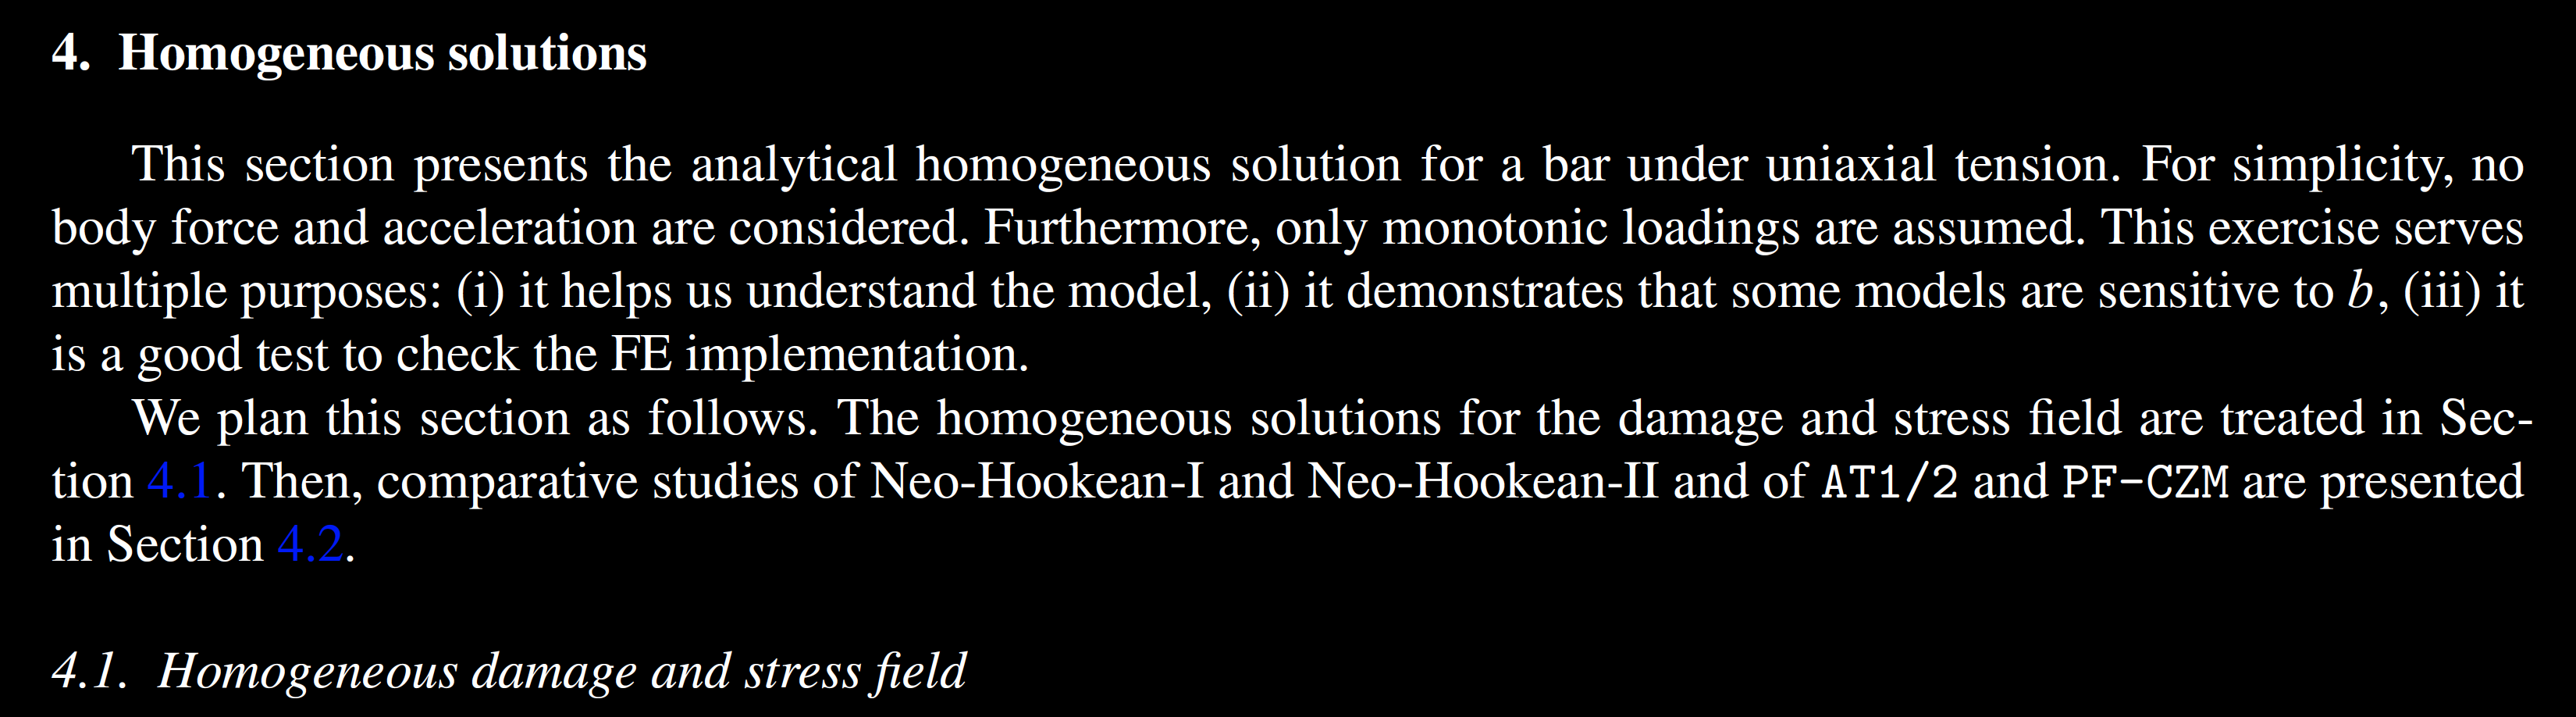
\includegraphics[width=0.9\textwidth]{section}
  \caption{A complex section should have a global paragraph between the heading of a section and the heading of its first subsection.}
  \label{fig:section}
\end{figure}


Papers on the field of computational engineering and sciences always have a section, typically named `Numerical Examples' where some tests are presented to demonstrate the performance of the model/theory presented. While these examples are most often presented in order of increasing complexity, we can do a better job in presenting them. For example, a global paragraph stating why these examples were chosen, which open source (if it is the case) code was used, etc. A table with all parameters used for all simulations would be helpful, see  \cref{table:params}.

\subsubsection{Introduction section}\label{sec:introduction-part}

Everyone would agree that the introductory section of a paper should contain the following items:

\begin{itemize}
\item What the problem that the paper is solving;
\item Demonstration the importance of that problem;
\item What are the current approaches to solving this problem and what is wrong about them;
\item What are the contributions of the paper; 
\item Planning  the readers for reading the subsequent sections.
\end{itemize}
in that order.

Writing an introductory section that simultaneously (i) includes all the above items, (ii) covers all relevant works, (iii) is easy to follow and (iv) is short is not an easy task.

What we commonly see is introductory sections of about 2 to 3 pages, full of just plain text with lots of jargons. There are two problems with this type of writing. First, only the authors and a dozens of experts can understand what is going on. Second, the paper loses many readers. We have realized that using some formula, figures, tables in the introduction section significantly improves the readability.
See \cref{algo-static-FEM} for an example, taken from \cite{Mandal:EFM2019}.

%---------------------------------------------------------------------------------------
\begin{MyBox}[label={algo-static-FEM}]
{Equations and tables can improve the introduction section.}
According to second-order PFMs for quasi-static fracture of solids under the infinitesimal strain regime, the displacement field $\bfu$ and damage field $d$ are minimisers of the following total energy functional of the solid 
\begin{equation*}
  \mathscr{E} (\bfu, d) 
    = \int_{\varOmega_{0}} \left[\omega(d)\psi_{0}^+(\bfepsilon (\bfu)) + \psi_{0}^-(\bfepsilon (\bfu)) \right]\td V
    + \int_{\varOmega_{0}}  \frac{G_\text{f}}{c_\alpha} \left[ \frac{1}{b} \alpha(d)
    + b \left( \nabla d \cdot \nabla d \right) \right] \td V
    - \mathscr{P} (\bfu)
\label{eq:3}
\end{equation*}
where the first integral is the stored strain energy, the second one denotes the fracture energy \`a la Griffith. The positive and negative parts of the strain energy density are denoted by $\psi_{0}^+(\bfepsilon (\bfu))$ and $\psi_{0}^-(\bfepsilon (\bfu))$, respectively.\\

 \begin{tabularx}{\textwidth}{lllllll}
   \toprule
 model & $\alpha(d)$ &  $\omega(d)$    & fracture type & length-scale & sup.  & Parameters\\
   \midrule     
  \texttt{AT2} & $d^2$  & $(1 - d)^{2}$  & brittle  & $b=(27/256) l_{\text{ch}}$ & $\infty$ & $E_0,\nu_0,G_\text{f},b$ \\
  \texttt{AT1} & $d$    & $(1 - d)^{2}$ &  brittle  & $b=(3/8) l_{\text{ch}}$ & $4b$  & $E_0,\nu_0,G_\text{f},b$\\
  \texttt{PF-CZM} & $2d-d^2$ & $\dfrac{(1 - d)^p}{(1 - d)^p + Q(d)}$ &  brittle/cohesive  & numerical param. & $\pi b$  & $E_0,\nu_0,G_\text{f},f_t$\\
   \bottomrule
 \end{tabularx}%
\end{MyBox}

One way to visually demonstrate the contributions of your paper is to use a table in which a comparison with existing models is given. We borrowed this idea from the computer graphics community, see e.g. \cite{Stomakhin:TG2013a}. Such a table is \cref{tab:summary} where we compared different variants of the material point method (MPM).

%%%%%%%%%%%%%%%%%%%%%%%%%%%%%%%%%%%%%%%%%%%%%%%%
\vspace*{3mm}
\begin{table*}[h!]
\centering
  \setlength\fboxsep{0pt}
\vskip-\topsep%
\smallskip%
%\renewcommand\arraystretch{1.3}
\colorbox{darkgray}{%
 \begin{tabularx}{0.99\textwidth}{lllllll}
   \toprule
 MPM variant & Efficiency & Quad. error & Cell crossing  & Num. fracture & Grid type & Contacts \\
   \midrule     
  MPM   & \smiley{} \smiley{}  \smiley{}  & \frownie{} \frownie{} \frownie{} & yes & yes & Cartesian/unstructured & \smiley{} \\
  GIMP  & \smiley{} \smiley{}  & \frownie{} \frownie{}   & no & yes  & Cartesian & \smiley{}  \\
  CPDI  & \smiley{} \smiley{}  & \frownie{}   & no  & no  & Cartesian&  \smiley{}  \\
  TLMPM & \smiley{} \smiley{} \smiley{} \smiley{}  & \frownie{}    & no & no  & Cartesian/unstructured&  \frownie{}   \\
  iMPM  & \smiley{}  & \frownie{}   & no & n/a & n/a & n/a \\
   \bottomrule
 \end{tabularx}%
}
 \caption{Overall characteristics of common MPM variants. The smileys and frownies are typeset using the package \texttt{wasysym}. }  
 \label{tab:summary}
\end{table*}

\subsubsection{Conclusion section}\label{sec:conclusion-part}

There are two misunderstandings about the Conclusion section. First, the Conclusion section is usually made long under the false belief that a longer Conclusion will seem more impressive. Second, it is most often just a replication of the Abstract and/or part of the Introduction in a present perfect tense. If the reader has to read your Conclusion to know what your paper is all about, then your Abstract and Introduction were not well written.

Some papers with well written sections even do not have a conclusion section. We are not a fan of that and believe having a conclusion is a good thing to do. Following the Nature paper introduced at the beginning of this section, a well written conclusion section should include the following items:

\begin{itemize}
\item One or two sentences summarizing what the paper has been about;
\item Summarizing the key findings of the paper;
\item What could be improved.
\end{itemize}

\subsubsection{Appendix and footnotes}\label{sec:appendix-footnotes}

It is appropriate to include appendices when
the incorporation of material in the body of the paper would make it poorly structured or it would be too long and detailed and to ensure inclusion of supporting material that would otherwise clutter or break up the narrative flow of the paper.
As discussed later in \cref{sec:equation}, it is better to move some equations to an appendix.

There are opposite ideas about footnotes. Some authors use them scarcely and some use them extensively. The argument of the former is that footnotes \textit{break the flow of thoughts and send your eyes darting back and forth while your hands are turning pages or clicking on links} according to Pulitzer prizewinner novelist Cormac McCarthy (see \url{https://www.nature.com/articles/d41586-019-02918-5}). The argument of the latter is probably to reduce the paper length. But, there is one thing wrong about footnotes: too lengthy footnotes. Some papers contain footnotes that are half page and with a smaller font, which are not readable.

We use footnotes sparingly and they are most often short. If you find a footnote long, consider using a remark as we have done in \cref{rm:a}.


% 
%--------------------------------------
\subsection{Some common mistakes}\label{sec:mistakes}


Some common mistakes are given in \cref{tab:mistakes}. You can avoid these mistakes by studying the writing style of your favorite author. Don't worry too much about grammatically perfect sentences. It is more important to be understood. \\

%%%%%%%%%%%%%%%%%%%%%%%%%%%%%%%%%%%%%%%%%%%%%%%%%%
\setlength{\fboxsep}{0pt}
\begin{table}[h!]
   \centering
     \setlength\fboxsep{0pt}
\vskip-\topsep%
\smallskip%
%\renewcommand\arraystretch{1.3}
\colorbox{darkgray}{%
   \begin{tabularx}{0.95\textwidth}{ll}
   \toprule
   Don't/Avoid & Do/Use  \\
  \midrule
  \textbf{The} Table/Figure 2 & Table/Figure 2 \\
  \textbf{The} Equation (2.2) & Equation (2.2) \\
  \textbf{The} Young's modulus &  Young's modulus, or the Young modulus\\
  Start a section with a table/figure/equation & Start a section with text\\
  This topic has interested researchers for a \textbf{long} time & ... for more than 20 years\\
  A \textbf{bad} result & A poor/negative result\\
  This section \textbf{serves} to explain & This section explains\\
  It is \textbf{obvious/clear} ... & \\
  \textbf{Due to the fact that} ... & Because ...\\
  \textbf{It should be noted that} there are 5 samples in this study& This study consisted of 5 ...\\
  \textbf{In order to} include ... & To include ...\\
  The difference was \textbf{found to be} significant & The difference was significant \\
  We plotted the data \textbf{by} using ... & We plotted the data using ...\\
  Utilize or usage & Use \\
  We \textbf{think/believe/feel} that the results are good & The results are good \\
  Using adjectives such as `very', `always', `never' & \\
  Using words like `ground-breaking', `paradigm shift' & \\ 
  Using 'Above-mentioned' or 'aforementioned' & \\
  Use long titles & Use short titles  \citep{paiva2012articles}\\
   & Use a spellchecker to get rid of all spell errors\\
  %Passive voice & Active voice \\
  \bottomrule
 \end{tabularx}%
 }
\caption{Some common mistakes.}
 \label{tab:mistakes}
\end{table}

Sentences can be described as active or passive. Using the passive voice is a way of writing sentences so that the subject has the action done to it. A common belief is that the passive voice can be useful for making writing sound more formal and objective. However, using it extensively results in papers which are boring with hard to understand lengthy sentences.

On the other hand, using a personal tone can help to engage a reader. And the sentences are shorter and thus easier to understand. 


%--------------------------------------
\subsection{Writing process: an iterative process}\label{sec:writing-process}

The first idea is when you have finished your last simulation, the first draft of your full paper is complete. Here, by \textit{you}, we mean the co-author of the paper who is in charge of the writing. After that, it is just polishing the paper. The second idea is to not lose motivation due to set backs. That is, if the simulations are not working, don't be upset; let's write something instead. It can be as easy as filling Section \textit{Acknowledgments}. Having updated your paper will definitely make you feel good. And that is very important. The third idea is that writing is intertwined with all other activities (formulation, coding and running simulations) as illustrated in \cref{fig:writing}.


After a research idea has been developed, you should start writing the paper \citep{Gray:2005a}. Obviously, the paper is empty, see \cref{snippet_template} for a \LaTeX\ file for an empty paper.
For the sake of presentation, let's assume that you need to develop a formulation, implement it in a code, and carry out simulations using this code. You first work on the formulation. Then, when there is some progresses, you can write some key equations in the paper (filling Section \textit{Methodology}). Having the formulations nicely written in a pdf can help you to spot errors. Now that the formulation is complete, let's move to the implementation. Again, this task should be intertwined  with the writing as well (filling Section \textit{Methodology}). Most often, you start with a very simple problem to test the code (and the idea). If this example works, you are confident about the idea, you can write something on Section \textit{Introduction} while the second simulation is under way. If this second example is important, you can write about it in Section \textit{Examples}. If you are lucky, the result of this second simulation is  good. Bingo, you can now fill  Sections \textit{Introduction} and  \textit{Abstract} while working on the third simulation.
%---------------------------------------------------------------------------
\begin{figure*}[!h]
  \begin{snippetlatex}[caption={A starting TEX file.},label={snippet_template},framerule=1pt,tabsize=3]
    \documentclass[authoryear,3p,times,preprint,review,fleqn]{elsarticle}
    \title{\textbf{}}
    \begin{abstract}
    \end{abstract}
    \section{Introduction}
    \section{Methodology}
    \section{Examples}
    \section{Conclusions}
    \section*{Acknowledgments}
    \bibliographystyle{abbrvnat} % bib style
    \bibliography{mpm}           % bib file
  \end{snippetlatex}
\end{figure*}
%---------------------------------------------------------------------------

 \begin{figure}[!ht]
      \centering
      \input{writing.pdf_tex}                 % insert a pdf_tex
      \caption{Writing is intertwined with other activities of the project.}
      \label{fig:writing}
    \end{figure}

If you feel stuck at writing any parts of the paper, feel free to do something else because keeping focusing on the writing does not always help. Most often, ideas come when you are in a diffuse mode, a concept proposed in \cite{Oakley:2018a}. For example, while playing with your kids on a playground, the idea for writing a good abstract usually comes. Jotting down the idea on a phone and you're done with this part of the paper.

While working on this paper, you read the literature (we always read it anyway). If you find a good paper relevant to your work, put it in \texttt{Bibdesk} or \texttt{JabRef}, and cite it in the paper with some key sentences about it. Doing so saves you a lot of time by not re-discovering this paper in the future. Note that \texttt{Bibdesk} can link a pdf to a paper. Therefore, we can have a library of papers on top of a \texttt{.bib} file. 

Continuing this process, by the time the final simulation has been finished, you already have a nearly complete paper. Note that you have already revised your paper many times when your simulations were running (which usually take a long time).
You just need to write the conclusions. And voila, you have a complete paper. Before submission, there are some steps discussed in \cref{sec:submission} that need to be done.

%%%%%%%%%%%%%%%%%%%%%%%%%%%%%%%
\section{\LaTeX\ tips}\label{sec:latex}

To improve the writing experience, once in a while one should update their \LaTeX\ skills. \cref{snippet_latex_packages} provides an updated list of \LaTeX\ packages being used to write our papers.
By setting the option \textit{backref=page} for the package \texttt{hyperref}, there appears `Cited on page \#' at the end of all references. 

Using standard cross-referencing in \LaTeX\ only produces the label number, a name describing the label such as figure, chapter or equation has to be added manually. The \texttt{cleveref} package overcomes this limitation by automatically producing the label name and number:

\begin{verbatim}
\cref{fig:figure1}, instead of Fig.~\ref{fig:figure1}
\cref{eq:equation1}, instead of Eq.~\ref{eq:equation1}
\end{verbatim}

%---------------------------------------------------------------------------
\begin{figure*}[!h]
  \begin{snippetlatex}[caption={Commonly used \LaTeX\ packages.},label={snippet_latex_packages},framerule=1pt,tabsize=3]
    \usepackage{amsmath,amssymb, mathtools,mathrsfs,stmaryrd,titletoc}
    \usepackage{natbib}
    \usepackage[scaled=0.92]{helvet}  % set Helvetica as the sans-serif font
    \renewcommand{\rmdefault}{ptm}    % set Times as the default text font
    \usepackage[retainorgcmds]{IEEEtrantools}
    \usepackage[usenames]{color}
    \usepackage{tabularx}
    \usepackage{booktabs}    % better tables
    \usepackage[font=small,labelfont=md]{caption,subfig} % sub-figures (see Fig. 6)
    \usepackage{multirow}
    \usepackage[T1]{fontenc} % typing french                        
    \usepackage[bookmarks=true,colorlinks=true,linkcolor=blue,backref=page]{hyperref}
    \usepackage{float}         % make new float environment such as boxes (captioned)
    \usepackage{listings}      % insert source code, used herein to insert LaTeX and Python codes 
    \usepackage{algorithm}
    \usepackage{algorithmicx}
    \usepackage{algpseudocode}
    %microtype: for Micro-Typographic Improvements
    \usepackage[activate={true,nocompatibility},final,tracking=true,kerning=true,
    spacing=true,factor=1100,stretch=10,shrink=10]{microtype}
    \usepackage{nicefrac}             % type inline fractions: \nicefrac{1}{2}
    \usepackage{numprint}             % \numprint{10000} => 10 000 not 10000
    \usepackage[capitalise]{cleveref} %Basically, cleveref must be loaded last.
    \definecolor{darkgray}{rgb}{0.95,0.95,0.95} % color used in tables
    % cleverref package: just do \cref{label} for figures, tables, equations anything
    % the package will determine the correct prefix be it Fig. or Equation or Listing.
    \crefname{figure}{Fig.}{Figs.}  
    \crefname{equation}{Equation}{Equations}

    \renewcommand*{\backref}[1]{}
    \renewcommand*{\backrefalt}[4]{[{%
        \ifcase #1 %
              \or Cited on page~#2%
              \else Cited on pages #2%
        \fi%
        }]}
  \end{snippetlatex}
\end{figure*}
%---------------------------------------------------------------------------

In what follows, we discuss how to prepare high quality plots in \cref{sec:figs}, tables in 
\cref{sec:tabs}. \cref{sec:equation} discusses notations and equations. Modifications required for preparing two-column format papers are presented in \cref{sec:two-col}.

%%%%%%%%%%%%%%%%%%%%%%
\subsection{Figures}\label{sec:figs}

It is not a requirement that the font used in figures match that of the text. Yet, it would be better if they match. \cref{fig:cold-spray-plot} is an example of a figure with non-matching text. The \LaTeX\ code used to include it in this paper is shown in \cref{snippet_latex_figure}. And the \texttt{Matplotlib} based \texttt{Python} script used to produce the PDF image with non-matching font is given in \cref{snippet_matplotlib}.
However, if you really want the font in your plots exactly match that in the text, see \cref{fig:cold-spray-plot-pgf} for such an example, the script in \cref{snippet_matplotlib_pgf} can be used.

%---------------------------------------------------------------------------
\begin{figure*}[!h]
  \begin{snippetlatex}[caption={\LaTeX\ commands to insert either a PDF, or PGF or PDF\_TEX image. The crucial point here is not to scale the inserted image. Otherwise, the font size will be affected.},label={snippet_latex_figure},framerule=1pt,tabsize=3]
    \begin{figure}[!ht]
      \centering
      % only one of the following three
      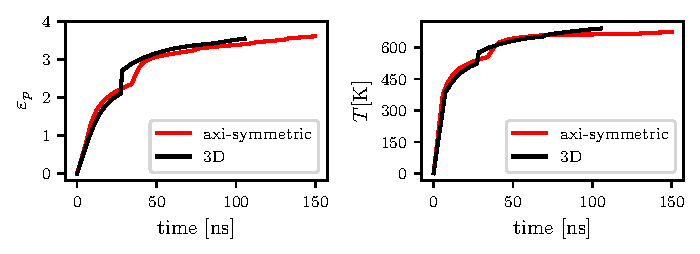
\includegraphics{cold-spray-plots.pdf} % insert a PDF
      %% Creator: Matplotlib, PGF backend
%%
%% To include the figure in your LaTeX document, write
%%   \input{<filename>.pgf}
%%
%% Make sure the required packages are loaded in your preamble
%%   \usepackage{pgf}
%%
%% Figures using additional raster images can only be included by \input if
%% they are in the same directory as the main LaTeX file. For loading figures
%% from other directories you can use the `import` package
%%   \usepackage{import}
%% and then include the figures with
%%   \import{<path to file>}{<filename>.pgf}
%%
%% Matplotlib used the following preamble
%%   \usepackage[utf8x]{inputenc}
%%   \usepackage[T1]{fontenc}
%%   \newcommand{\vect}[1]{#1}
%%
\begingroup%
\makeatletter%
\begin{pgfpicture}%
\pgfpathrectangle{\pgfpointorigin}{\pgfqpoint{6.375716in}{2.328394in}}%
\pgfusepath{use as bounding box, clip}%
\begin{pgfscope}%
\pgfsetbuttcap%
\pgfsetmiterjoin%
\definecolor{currentfill}{rgb}{1.000000,1.000000,1.000000}%
\pgfsetfillcolor{currentfill}%
\pgfsetlinewidth{0.000000pt}%
\definecolor{currentstroke}{rgb}{1.000000,1.000000,1.000000}%
\pgfsetstrokecolor{currentstroke}%
\pgfsetdash{}{0pt}%
\pgfpathmoveto{\pgfqpoint{0.000000in}{0.000000in}}%
\pgfpathlineto{\pgfqpoint{6.375716in}{0.000000in}}%
\pgfpathlineto{\pgfqpoint{6.375716in}{2.328394in}}%
\pgfpathlineto{\pgfqpoint{0.000000in}{2.328394in}}%
\pgfpathclose%
\pgfusepath{fill}%
\end{pgfscope}%
\begin{pgfscope}%
\pgfsetbuttcap%
\pgfsetmiterjoin%
\definecolor{currentfill}{rgb}{1.000000,1.000000,1.000000}%
\pgfsetfillcolor{currentfill}%
\pgfsetlinewidth{0.000000pt}%
\definecolor{currentstroke}{rgb}{0.000000,0.000000,0.000000}%
\pgfsetstrokecolor{currentstroke}%
\pgfsetstrokeopacity{0.000000}%
\pgfsetdash{}{0pt}%
\pgfpathmoveto{\pgfqpoint{0.434462in}{0.489757in}}%
\pgfpathlineto{\pgfqpoint{3.045729in}{0.489757in}}%
\pgfpathlineto{\pgfqpoint{3.045729in}{2.190131in}}%
\pgfpathlineto{\pgfqpoint{0.434462in}{2.190131in}}%
\pgfpathclose%
\pgfusepath{fill}%
\end{pgfscope}%
\begin{pgfscope}%
\pgfsetbuttcap%
\pgfsetroundjoin%
\definecolor{currentfill}{rgb}{0.000000,0.000000,0.000000}%
\pgfsetfillcolor{currentfill}%
\pgfsetlinewidth{0.803000pt}%
\definecolor{currentstroke}{rgb}{0.000000,0.000000,0.000000}%
\pgfsetstrokecolor{currentstroke}%
\pgfsetdash{}{0pt}%
\pgfsys@defobject{currentmarker}{\pgfqpoint{0.000000in}{-0.048611in}}{\pgfqpoint{0.000000in}{0.000000in}}{%
\pgfpathmoveto{\pgfqpoint{0.000000in}{0.000000in}}%
\pgfpathlineto{\pgfqpoint{0.000000in}{-0.048611in}}%
\pgfusepath{stroke,fill}%
}%
\begin{pgfscope}%
\pgfsys@transformshift{0.553156in}{0.489757in}%
\pgfsys@useobject{currentmarker}{}%
\end{pgfscope}%
\end{pgfscope}%
\begin{pgfscope}%
\definecolor{textcolor}{rgb}{0.000000,0.000000,0.000000}%
\pgfsetstrokecolor{textcolor}%
\pgfsetfillcolor{textcolor}%
\pgftext[x=0.553156in,y=0.392535in,,top]{\color{textcolor}\rmfamily\fontsize{8.000000}{9.600000}\selectfont \(\displaystyle 0\)}%
\end{pgfscope}%
\begin{pgfscope}%
\pgfsetbuttcap%
\pgfsetroundjoin%
\definecolor{currentfill}{rgb}{0.000000,0.000000,0.000000}%
\pgfsetfillcolor{currentfill}%
\pgfsetlinewidth{0.803000pt}%
\definecolor{currentstroke}{rgb}{0.000000,0.000000,0.000000}%
\pgfsetstrokecolor{currentstroke}%
\pgfsetdash{}{0pt}%
\pgfsys@defobject{currentmarker}{\pgfqpoint{0.000000in}{-0.048611in}}{\pgfqpoint{0.000000in}{0.000000in}}{%
\pgfpathmoveto{\pgfqpoint{0.000000in}{0.000000in}}%
\pgfpathlineto{\pgfqpoint{0.000000in}{-0.048611in}}%
\pgfusepath{stroke,fill}%
}%
\begin{pgfscope}%
\pgfsys@transformshift{0.948881in}{0.489757in}%
\pgfsys@useobject{currentmarker}{}%
\end{pgfscope}%
\end{pgfscope}%
\begin{pgfscope}%
\definecolor{textcolor}{rgb}{0.000000,0.000000,0.000000}%
\pgfsetstrokecolor{textcolor}%
\pgfsetfillcolor{textcolor}%
\pgftext[x=0.948881in,y=0.392535in,,top]{\color{textcolor}\rmfamily\fontsize{8.000000}{9.600000}\selectfont \(\displaystyle 25\)}%
\end{pgfscope}%
\begin{pgfscope}%
\pgfsetbuttcap%
\pgfsetroundjoin%
\definecolor{currentfill}{rgb}{0.000000,0.000000,0.000000}%
\pgfsetfillcolor{currentfill}%
\pgfsetlinewidth{0.803000pt}%
\definecolor{currentstroke}{rgb}{0.000000,0.000000,0.000000}%
\pgfsetstrokecolor{currentstroke}%
\pgfsetdash{}{0pt}%
\pgfsys@defobject{currentmarker}{\pgfqpoint{0.000000in}{-0.048611in}}{\pgfqpoint{0.000000in}{0.000000in}}{%
\pgfpathmoveto{\pgfqpoint{0.000000in}{0.000000in}}%
\pgfpathlineto{\pgfqpoint{0.000000in}{-0.048611in}}%
\pgfusepath{stroke,fill}%
}%
\begin{pgfscope}%
\pgfsys@transformshift{1.344607in}{0.489757in}%
\pgfsys@useobject{currentmarker}{}%
\end{pgfscope}%
\end{pgfscope}%
\begin{pgfscope}%
\definecolor{textcolor}{rgb}{0.000000,0.000000,0.000000}%
\pgfsetstrokecolor{textcolor}%
\pgfsetfillcolor{textcolor}%
\pgftext[x=1.344607in,y=0.392535in,,top]{\color{textcolor}\rmfamily\fontsize{8.000000}{9.600000}\selectfont \(\displaystyle 50\)}%
\end{pgfscope}%
\begin{pgfscope}%
\pgfsetbuttcap%
\pgfsetroundjoin%
\definecolor{currentfill}{rgb}{0.000000,0.000000,0.000000}%
\pgfsetfillcolor{currentfill}%
\pgfsetlinewidth{0.803000pt}%
\definecolor{currentstroke}{rgb}{0.000000,0.000000,0.000000}%
\pgfsetstrokecolor{currentstroke}%
\pgfsetdash{}{0pt}%
\pgfsys@defobject{currentmarker}{\pgfqpoint{0.000000in}{-0.048611in}}{\pgfqpoint{0.000000in}{0.000000in}}{%
\pgfpathmoveto{\pgfqpoint{0.000000in}{0.000000in}}%
\pgfpathlineto{\pgfqpoint{0.000000in}{-0.048611in}}%
\pgfusepath{stroke,fill}%
}%
\begin{pgfscope}%
\pgfsys@transformshift{1.740333in}{0.489757in}%
\pgfsys@useobject{currentmarker}{}%
\end{pgfscope}%
\end{pgfscope}%
\begin{pgfscope}%
\definecolor{textcolor}{rgb}{0.000000,0.000000,0.000000}%
\pgfsetstrokecolor{textcolor}%
\pgfsetfillcolor{textcolor}%
\pgftext[x=1.740333in,y=0.392535in,,top]{\color{textcolor}\rmfamily\fontsize{8.000000}{9.600000}\selectfont \(\displaystyle 75\)}%
\end{pgfscope}%
\begin{pgfscope}%
\pgfsetbuttcap%
\pgfsetroundjoin%
\definecolor{currentfill}{rgb}{0.000000,0.000000,0.000000}%
\pgfsetfillcolor{currentfill}%
\pgfsetlinewidth{0.803000pt}%
\definecolor{currentstroke}{rgb}{0.000000,0.000000,0.000000}%
\pgfsetstrokecolor{currentstroke}%
\pgfsetdash{}{0pt}%
\pgfsys@defobject{currentmarker}{\pgfqpoint{0.000000in}{-0.048611in}}{\pgfqpoint{0.000000in}{0.000000in}}{%
\pgfpathmoveto{\pgfqpoint{0.000000in}{0.000000in}}%
\pgfpathlineto{\pgfqpoint{0.000000in}{-0.048611in}}%
\pgfusepath{stroke,fill}%
}%
\begin{pgfscope}%
\pgfsys@transformshift{2.136059in}{0.489757in}%
\pgfsys@useobject{currentmarker}{}%
\end{pgfscope}%
\end{pgfscope}%
\begin{pgfscope}%
\definecolor{textcolor}{rgb}{0.000000,0.000000,0.000000}%
\pgfsetstrokecolor{textcolor}%
\pgfsetfillcolor{textcolor}%
\pgftext[x=2.136059in,y=0.392535in,,top]{\color{textcolor}\rmfamily\fontsize{8.000000}{9.600000}\selectfont \(\displaystyle 100\)}%
\end{pgfscope}%
\begin{pgfscope}%
\pgfsetbuttcap%
\pgfsetroundjoin%
\definecolor{currentfill}{rgb}{0.000000,0.000000,0.000000}%
\pgfsetfillcolor{currentfill}%
\pgfsetlinewidth{0.803000pt}%
\definecolor{currentstroke}{rgb}{0.000000,0.000000,0.000000}%
\pgfsetstrokecolor{currentstroke}%
\pgfsetdash{}{0pt}%
\pgfsys@defobject{currentmarker}{\pgfqpoint{0.000000in}{-0.048611in}}{\pgfqpoint{0.000000in}{0.000000in}}{%
\pgfpathmoveto{\pgfqpoint{0.000000in}{0.000000in}}%
\pgfpathlineto{\pgfqpoint{0.000000in}{-0.048611in}}%
\pgfusepath{stroke,fill}%
}%
\begin{pgfscope}%
\pgfsys@transformshift{2.531785in}{0.489757in}%
\pgfsys@useobject{currentmarker}{}%
\end{pgfscope}%
\end{pgfscope}%
\begin{pgfscope}%
\definecolor{textcolor}{rgb}{0.000000,0.000000,0.000000}%
\pgfsetstrokecolor{textcolor}%
\pgfsetfillcolor{textcolor}%
\pgftext[x=2.531785in,y=0.392535in,,top]{\color{textcolor}\rmfamily\fontsize{8.000000}{9.600000}\selectfont \(\displaystyle 125\)}%
\end{pgfscope}%
\begin{pgfscope}%
\pgfsetbuttcap%
\pgfsetroundjoin%
\definecolor{currentfill}{rgb}{0.000000,0.000000,0.000000}%
\pgfsetfillcolor{currentfill}%
\pgfsetlinewidth{0.803000pt}%
\definecolor{currentstroke}{rgb}{0.000000,0.000000,0.000000}%
\pgfsetstrokecolor{currentstroke}%
\pgfsetdash{}{0pt}%
\pgfsys@defobject{currentmarker}{\pgfqpoint{0.000000in}{-0.048611in}}{\pgfqpoint{0.000000in}{0.000000in}}{%
\pgfpathmoveto{\pgfqpoint{0.000000in}{0.000000in}}%
\pgfpathlineto{\pgfqpoint{0.000000in}{-0.048611in}}%
\pgfusepath{stroke,fill}%
}%
\begin{pgfscope}%
\pgfsys@transformshift{2.927510in}{0.489757in}%
\pgfsys@useobject{currentmarker}{}%
\end{pgfscope}%
\end{pgfscope}%
\begin{pgfscope}%
\definecolor{textcolor}{rgb}{0.000000,0.000000,0.000000}%
\pgfsetstrokecolor{textcolor}%
\pgfsetfillcolor{textcolor}%
\pgftext[x=2.927510in,y=0.392535in,,top]{\color{textcolor}\rmfamily\fontsize{8.000000}{9.600000}\selectfont \(\displaystyle 150\)}%
\end{pgfscope}%
\begin{pgfscope}%
\definecolor{textcolor}{rgb}{0.000000,0.000000,0.000000}%
\pgfsetstrokecolor{textcolor}%
\pgfsetfillcolor{textcolor}%
\pgftext[x=1.740096in,y=0.238855in,,top]{\color{textcolor}\rmfamily\fontsize{10.000000}{12.000000}\selectfont time [ns]}%
\end{pgfscope}%
\begin{pgfscope}%
\pgfsetbuttcap%
\pgfsetroundjoin%
\definecolor{currentfill}{rgb}{0.000000,0.000000,0.000000}%
\pgfsetfillcolor{currentfill}%
\pgfsetlinewidth{0.803000pt}%
\definecolor{currentstroke}{rgb}{0.000000,0.000000,0.000000}%
\pgfsetstrokecolor{currentstroke}%
\pgfsetdash{}{0pt}%
\pgfsys@defobject{currentmarker}{\pgfqpoint{-0.048611in}{0.000000in}}{\pgfqpoint{0.000000in}{0.000000in}}{%
\pgfpathmoveto{\pgfqpoint{0.000000in}{0.000000in}}%
\pgfpathlineto{\pgfqpoint{-0.048611in}{0.000000in}}%
\pgfusepath{stroke,fill}%
}%
\begin{pgfscope}%
\pgfsys@transformshift{0.434462in}{0.563078in}%
\pgfsys@useobject{currentmarker}{}%
\end{pgfscope}%
\end{pgfscope}%
\begin{pgfscope}%
\definecolor{textcolor}{rgb}{0.000000,0.000000,0.000000}%
\pgfsetstrokecolor{textcolor}%
\pgfsetfillcolor{textcolor}%
\pgftext[x=0.278211in,y=0.524816in,left,base]{\color{textcolor}\rmfamily\fontsize{8.000000}{9.600000}\selectfont \(\displaystyle 0\)}%
\end{pgfscope}%
\begin{pgfscope}%
\pgfsetbuttcap%
\pgfsetroundjoin%
\definecolor{currentfill}{rgb}{0.000000,0.000000,0.000000}%
\pgfsetfillcolor{currentfill}%
\pgfsetlinewidth{0.803000pt}%
\definecolor{currentstroke}{rgb}{0.000000,0.000000,0.000000}%
\pgfsetstrokecolor{currentstroke}%
\pgfsetdash{}{0pt}%
\pgfsys@defobject{currentmarker}{\pgfqpoint{-0.048611in}{0.000000in}}{\pgfqpoint{0.000000in}{0.000000in}}{%
\pgfpathmoveto{\pgfqpoint{0.000000in}{0.000000in}}%
\pgfpathlineto{\pgfqpoint{-0.048611in}{0.000000in}}%
\pgfusepath{stroke,fill}%
}%
\begin{pgfscope}%
\pgfsys@transformshift{0.434462in}{0.969841in}%
\pgfsys@useobject{currentmarker}{}%
\end{pgfscope}%
\end{pgfscope}%
\begin{pgfscope}%
\definecolor{textcolor}{rgb}{0.000000,0.000000,0.000000}%
\pgfsetstrokecolor{textcolor}%
\pgfsetfillcolor{textcolor}%
\pgftext[x=0.278211in,y=0.931579in,left,base]{\color{textcolor}\rmfamily\fontsize{8.000000}{9.600000}\selectfont \(\displaystyle 1\)}%
\end{pgfscope}%
\begin{pgfscope}%
\pgfsetbuttcap%
\pgfsetroundjoin%
\definecolor{currentfill}{rgb}{0.000000,0.000000,0.000000}%
\pgfsetfillcolor{currentfill}%
\pgfsetlinewidth{0.803000pt}%
\definecolor{currentstroke}{rgb}{0.000000,0.000000,0.000000}%
\pgfsetstrokecolor{currentstroke}%
\pgfsetdash{}{0pt}%
\pgfsys@defobject{currentmarker}{\pgfqpoint{-0.048611in}{0.000000in}}{\pgfqpoint{0.000000in}{0.000000in}}{%
\pgfpathmoveto{\pgfqpoint{0.000000in}{0.000000in}}%
\pgfpathlineto{\pgfqpoint{-0.048611in}{0.000000in}}%
\pgfusepath{stroke,fill}%
}%
\begin{pgfscope}%
\pgfsys@transformshift{0.434462in}{1.376605in}%
\pgfsys@useobject{currentmarker}{}%
\end{pgfscope}%
\end{pgfscope}%
\begin{pgfscope}%
\definecolor{textcolor}{rgb}{0.000000,0.000000,0.000000}%
\pgfsetstrokecolor{textcolor}%
\pgfsetfillcolor{textcolor}%
\pgftext[x=0.278211in,y=1.338342in,left,base]{\color{textcolor}\rmfamily\fontsize{8.000000}{9.600000}\selectfont \(\displaystyle 2\)}%
\end{pgfscope}%
\begin{pgfscope}%
\pgfsetbuttcap%
\pgfsetroundjoin%
\definecolor{currentfill}{rgb}{0.000000,0.000000,0.000000}%
\pgfsetfillcolor{currentfill}%
\pgfsetlinewidth{0.803000pt}%
\definecolor{currentstroke}{rgb}{0.000000,0.000000,0.000000}%
\pgfsetstrokecolor{currentstroke}%
\pgfsetdash{}{0pt}%
\pgfsys@defobject{currentmarker}{\pgfqpoint{-0.048611in}{0.000000in}}{\pgfqpoint{0.000000in}{0.000000in}}{%
\pgfpathmoveto{\pgfqpoint{0.000000in}{0.000000in}}%
\pgfpathlineto{\pgfqpoint{-0.048611in}{0.000000in}}%
\pgfusepath{stroke,fill}%
}%
\begin{pgfscope}%
\pgfsys@transformshift{0.434462in}{1.783368in}%
\pgfsys@useobject{currentmarker}{}%
\end{pgfscope}%
\end{pgfscope}%
\begin{pgfscope}%
\definecolor{textcolor}{rgb}{0.000000,0.000000,0.000000}%
\pgfsetstrokecolor{textcolor}%
\pgfsetfillcolor{textcolor}%
\pgftext[x=0.278211in,y=1.745106in,left,base]{\color{textcolor}\rmfamily\fontsize{8.000000}{9.600000}\selectfont \(\displaystyle 3\)}%
\end{pgfscope}%
\begin{pgfscope}%
\pgfsetbuttcap%
\pgfsetroundjoin%
\definecolor{currentfill}{rgb}{0.000000,0.000000,0.000000}%
\pgfsetfillcolor{currentfill}%
\pgfsetlinewidth{0.803000pt}%
\definecolor{currentstroke}{rgb}{0.000000,0.000000,0.000000}%
\pgfsetstrokecolor{currentstroke}%
\pgfsetdash{}{0pt}%
\pgfsys@defobject{currentmarker}{\pgfqpoint{-0.048611in}{0.000000in}}{\pgfqpoint{0.000000in}{0.000000in}}{%
\pgfpathmoveto{\pgfqpoint{0.000000in}{0.000000in}}%
\pgfpathlineto{\pgfqpoint{-0.048611in}{0.000000in}}%
\pgfusepath{stroke,fill}%
}%
\begin{pgfscope}%
\pgfsys@transformshift{0.434462in}{2.190131in}%
\pgfsys@useobject{currentmarker}{}%
\end{pgfscope}%
\end{pgfscope}%
\begin{pgfscope}%
\definecolor{textcolor}{rgb}{0.000000,0.000000,0.000000}%
\pgfsetstrokecolor{textcolor}%
\pgfsetfillcolor{textcolor}%
\pgftext[x=0.278211in,y=2.151869in,left,base]{\color{textcolor}\rmfamily\fontsize{8.000000}{9.600000}\selectfont \(\displaystyle 4\)}%
\end{pgfscope}%
\begin{pgfscope}%
\definecolor{textcolor}{rgb}{0.000000,0.000000,0.000000}%
\pgfsetstrokecolor{textcolor}%
\pgfsetfillcolor{textcolor}%
\pgftext[x=0.222655in,y=1.339944in,,bottom,rotate=90.000000]{\color{textcolor}\rmfamily\fontsize{10.000000}{12.000000}\selectfont \(\displaystyle \varepsilon_p\)}%
\end{pgfscope}%
\begin{pgfscope}%
\pgfpathrectangle{\pgfqpoint{0.434462in}{0.489757in}}{\pgfqpoint{2.611268in}{1.700374in}}%
\pgfusepath{clip}%
\pgfsetrectcap%
\pgfsetroundjoin%
\pgfsetlinewidth{1.505625pt}%
\definecolor{currentstroke}{rgb}{1.000000,0.000000,0.000000}%
\pgfsetstrokecolor{currentstroke}%
\pgfsetdash{}{0pt}%
\pgfpathmoveto{\pgfqpoint{0.553156in}{0.563078in}}%
\pgfpathlineto{\pgfqpoint{0.644136in}{0.898446in}}%
\pgfpathlineto{\pgfqpoint{0.677856in}{1.049453in}}%
\pgfpathlineto{\pgfqpoint{0.701275in}{1.128621in}}%
\pgfpathlineto{\pgfqpoint{0.720070in}{1.178198in}}%
\pgfpathlineto{\pgfqpoint{0.750463in}{1.247038in}}%
\pgfpathlineto{\pgfqpoint{0.763527in}{1.269512in}}%
\pgfpathlineto{\pgfqpoint{0.787471in}{1.301349in}}%
\pgfpathlineto{\pgfqpoint{0.819226in}{1.343112in}}%
\pgfpathlineto{\pgfqpoint{0.838567in}{1.361445in}}%
\pgfpathlineto{\pgfqpoint{0.899727in}{1.413807in}}%
\pgfpathlineto{\pgfqpoint{0.923829in}{1.429057in}}%
\pgfpathlineto{\pgfqpoint{0.946966in}{1.443696in}}%
\pgfpathlineto{\pgfqpoint{0.961875in}{1.454223in}}%
\pgfpathlineto{\pgfqpoint{0.983819in}{1.465991in}}%
\pgfpathlineto{\pgfqpoint{1.019222in}{1.483819in}}%
\pgfpathlineto{\pgfqpoint{1.032951in}{1.491572in}}%
\pgfpathlineto{\pgfqpoint{1.053315in}{1.500452in}}%
\pgfpathlineto{\pgfqpoint{1.086542in}{1.514200in}}%
\pgfpathlineto{\pgfqpoint{1.093049in}{1.517463in}}%
\pgfpathlineto{\pgfqpoint{1.099529in}{1.524715in}}%
\pgfpathlineto{\pgfqpoint{1.125278in}{1.594898in}}%
\pgfpathlineto{\pgfqpoint{1.144395in}{1.640806in}}%
\pgfpathlineto{\pgfqpoint{1.163208in}{1.678936in}}%
\pgfpathlineto{\pgfqpoint{1.181844in}{1.710216in}}%
\pgfpathlineto{\pgfqpoint{1.194230in}{1.728805in}}%
\pgfpathlineto{\pgfqpoint{1.206584in}{1.743741in}}%
\pgfpathlineto{\pgfqpoint{1.218857in}{1.753093in}}%
\pgfpathlineto{\pgfqpoint{1.254602in}{1.776233in}}%
\pgfpathlineto{\pgfqpoint{1.272082in}{1.786492in}}%
\pgfpathlineto{\pgfqpoint{1.289316in}{1.793944in}}%
\pgfpathlineto{\pgfqpoint{1.322880in}{1.804577in}}%
\pgfpathlineto{\pgfqpoint{1.361164in}{1.814729in}}%
\pgfpathlineto{\pgfqpoint{1.461503in}{1.836996in}}%
\pgfpathlineto{\pgfqpoint{1.523974in}{1.848283in}}%
\pgfpathlineto{\pgfqpoint{1.581436in}{1.856642in}}%
\pgfpathlineto{\pgfqpoint{1.655624in}{1.867027in}}%
\pgfpathlineto{\pgfqpoint{1.704159in}{1.877143in}}%
\pgfpathlineto{\pgfqpoint{1.720447in}{1.882065in}}%
\pgfpathlineto{\pgfqpoint{1.731353in}{1.887589in}}%
\pgfpathlineto{\pgfqpoint{1.736822in}{1.894923in}}%
\pgfpathlineto{\pgfqpoint{1.792102in}{1.902875in}}%
\pgfpathlineto{\pgfqpoint{1.888103in}{1.914395in}}%
\pgfpathlineto{\pgfqpoint{1.974797in}{1.922213in}}%
\pgfpathlineto{\pgfqpoint{2.105240in}{1.933289in}}%
\pgfpathlineto{\pgfqpoint{2.269941in}{1.950580in}}%
\pgfpathlineto{\pgfqpoint{2.307076in}{1.956071in}}%
\pgfpathlineto{\pgfqpoint{2.325738in}{1.960619in}}%
\pgfpathlineto{\pgfqpoint{2.338211in}{1.967221in}}%
\pgfpathlineto{\pgfqpoint{2.438726in}{1.974868in}}%
\pgfpathlineto{\pgfqpoint{2.598203in}{1.991277in}}%
\pgfpathlineto{\pgfqpoint{2.630368in}{1.996601in}}%
\pgfpathlineto{\pgfqpoint{2.643253in}{2.001076in}}%
\pgfpathlineto{\pgfqpoint{2.649711in}{2.006563in}}%
\pgfpathlineto{\pgfqpoint{2.830542in}{2.022651in}}%
\pgfpathlineto{\pgfqpoint{2.927035in}{2.029496in}}%
\pgfpathlineto{\pgfqpoint{2.927035in}{2.029496in}}%
\pgfusepath{stroke}%
\end{pgfscope}%
\begin{pgfscope}%
\pgfsetrectcap%
\pgfsetmiterjoin%
\pgfsetlinewidth{0.803000pt}%
\definecolor{currentstroke}{rgb}{0.000000,0.000000,0.000000}%
\pgfsetstrokecolor{currentstroke}%
\pgfsetdash{}{0pt}%
\pgfpathmoveto{\pgfqpoint{0.434462in}{0.489757in}}%
\pgfpathlineto{\pgfqpoint{0.434462in}{2.190131in}}%
\pgfusepath{stroke}%
\end{pgfscope}%
\begin{pgfscope}%
\pgfsetrectcap%
\pgfsetmiterjoin%
\pgfsetlinewidth{0.803000pt}%
\definecolor{currentstroke}{rgb}{0.000000,0.000000,0.000000}%
\pgfsetstrokecolor{currentstroke}%
\pgfsetdash{}{0pt}%
\pgfpathmoveto{\pgfqpoint{3.045729in}{0.489757in}}%
\pgfpathlineto{\pgfqpoint{3.045729in}{2.190131in}}%
\pgfusepath{stroke}%
\end{pgfscope}%
\begin{pgfscope}%
\pgfsetrectcap%
\pgfsetmiterjoin%
\pgfsetlinewidth{0.803000pt}%
\definecolor{currentstroke}{rgb}{0.000000,0.000000,0.000000}%
\pgfsetstrokecolor{currentstroke}%
\pgfsetdash{}{0pt}%
\pgfpathmoveto{\pgfqpoint{0.434462in}{0.489757in}}%
\pgfpathlineto{\pgfqpoint{3.045729in}{0.489757in}}%
\pgfusepath{stroke}%
\end{pgfscope}%
\begin{pgfscope}%
\pgfsetrectcap%
\pgfsetmiterjoin%
\pgfsetlinewidth{0.803000pt}%
\definecolor{currentstroke}{rgb}{0.000000,0.000000,0.000000}%
\pgfsetstrokecolor{currentstroke}%
\pgfsetdash{}{0pt}%
\pgfpathmoveto{\pgfqpoint{0.434462in}{2.190131in}}%
\pgfpathlineto{\pgfqpoint{3.045729in}{2.190131in}}%
\pgfusepath{stroke}%
\end{pgfscope}%
\begin{pgfscope}%
\pgfsetbuttcap%
\pgfsetmiterjoin%
\definecolor{currentfill}{rgb}{1.000000,1.000000,1.000000}%
\pgfsetfillcolor{currentfill}%
\pgfsetfillopacity{0.800000}%
\pgfsetlinewidth{1.003750pt}%
\definecolor{currentstroke}{rgb}{0.800000,0.800000,0.800000}%
\pgfsetstrokecolor{currentstroke}%
\pgfsetstrokeopacity{0.800000}%
\pgfsetdash{}{0pt}%
\pgfpathmoveto{\pgfqpoint{0.512239in}{1.946309in}}%
\pgfpathlineto{\pgfqpoint{1.596378in}{1.946309in}}%
\pgfpathquadraticcurveto{\pgfqpoint{1.618601in}{1.946309in}}{\pgfqpoint{1.618601in}{1.968532in}}%
\pgfpathlineto{\pgfqpoint{1.618601in}{2.112353in}}%
\pgfpathquadraticcurveto{\pgfqpoint{1.618601in}{2.134576in}}{\pgfqpoint{1.596378in}{2.134576in}}%
\pgfpathlineto{\pgfqpoint{0.512239in}{2.134576in}}%
\pgfpathquadraticcurveto{\pgfqpoint{0.490017in}{2.134576in}}{\pgfqpoint{0.490017in}{2.112353in}}%
\pgfpathlineto{\pgfqpoint{0.490017in}{1.968532in}}%
\pgfpathquadraticcurveto{\pgfqpoint{0.490017in}{1.946309in}}{\pgfqpoint{0.512239in}{1.946309in}}%
\pgfpathclose%
\pgfusepath{stroke,fill}%
\end{pgfscope}%
\begin{pgfscope}%
\pgfsetrectcap%
\pgfsetroundjoin%
\pgfsetlinewidth{1.505625pt}%
\definecolor{currentstroke}{rgb}{1.000000,0.000000,0.000000}%
\pgfsetstrokecolor{currentstroke}%
\pgfsetdash{}{0pt}%
\pgfpathmoveto{\pgfqpoint{0.534462in}{2.051242in}}%
\pgfpathlineto{\pgfqpoint{0.756684in}{2.051242in}}%
\pgfusepath{stroke}%
\end{pgfscope}%
\begin{pgfscope}%
\definecolor{textcolor}{rgb}{0.000000,0.000000,0.000000}%
\pgfsetstrokecolor{textcolor}%
\pgfsetfillcolor{textcolor}%
\pgftext[x=0.845573in,y=2.012353in,left,base]{\color{textcolor}\rmfamily\fontsize{8.000000}{9.600000}\selectfont axi-symmetric}%
\end{pgfscope}%
\begin{pgfscope}%
\pgfsetbuttcap%
\pgfsetmiterjoin%
\definecolor{currentfill}{rgb}{1.000000,1.000000,1.000000}%
\pgfsetfillcolor{currentfill}%
\pgfsetlinewidth{0.000000pt}%
\definecolor{currentstroke}{rgb}{0.000000,0.000000,0.000000}%
\pgfsetstrokecolor{currentstroke}%
\pgfsetstrokeopacity{0.000000}%
\pgfsetdash{}{0pt}%
\pgfpathmoveto{\pgfqpoint{3.664448in}{0.489757in}}%
\pgfpathlineto{\pgfqpoint{6.275716in}{0.489757in}}%
\pgfpathlineto{\pgfqpoint{6.275716in}{2.190131in}}%
\pgfpathlineto{\pgfqpoint{3.664448in}{2.190131in}}%
\pgfpathclose%
\pgfusepath{fill}%
\end{pgfscope}%
\begin{pgfscope}%
\pgfsetbuttcap%
\pgfsetroundjoin%
\definecolor{currentfill}{rgb}{0.000000,0.000000,0.000000}%
\pgfsetfillcolor{currentfill}%
\pgfsetlinewidth{0.803000pt}%
\definecolor{currentstroke}{rgb}{0.000000,0.000000,0.000000}%
\pgfsetstrokecolor{currentstroke}%
\pgfsetdash{}{0pt}%
\pgfsys@defobject{currentmarker}{\pgfqpoint{0.000000in}{-0.048611in}}{\pgfqpoint{0.000000in}{0.000000in}}{%
\pgfpathmoveto{\pgfqpoint{0.000000in}{0.000000in}}%
\pgfpathlineto{\pgfqpoint{0.000000in}{-0.048611in}}%
\pgfusepath{stroke,fill}%
}%
\begin{pgfscope}%
\pgfsys@transformshift{3.783142in}{0.489757in}%
\pgfsys@useobject{currentmarker}{}%
\end{pgfscope}%
\end{pgfscope}%
\begin{pgfscope}%
\definecolor{textcolor}{rgb}{0.000000,0.000000,0.000000}%
\pgfsetstrokecolor{textcolor}%
\pgfsetfillcolor{textcolor}%
\pgftext[x=3.783142in,y=0.392535in,,top]{\color{textcolor}\rmfamily\fontsize{8.000000}{9.600000}\selectfont \(\displaystyle 0\)}%
\end{pgfscope}%
\begin{pgfscope}%
\pgfsetbuttcap%
\pgfsetroundjoin%
\definecolor{currentfill}{rgb}{0.000000,0.000000,0.000000}%
\pgfsetfillcolor{currentfill}%
\pgfsetlinewidth{0.803000pt}%
\definecolor{currentstroke}{rgb}{0.000000,0.000000,0.000000}%
\pgfsetstrokecolor{currentstroke}%
\pgfsetdash{}{0pt}%
\pgfsys@defobject{currentmarker}{\pgfqpoint{0.000000in}{-0.048611in}}{\pgfqpoint{0.000000in}{0.000000in}}{%
\pgfpathmoveto{\pgfqpoint{0.000000in}{0.000000in}}%
\pgfpathlineto{\pgfqpoint{0.000000in}{-0.048611in}}%
\pgfusepath{stroke,fill}%
}%
\begin{pgfscope}%
\pgfsys@transformshift{4.178868in}{0.489757in}%
\pgfsys@useobject{currentmarker}{}%
\end{pgfscope}%
\end{pgfscope}%
\begin{pgfscope}%
\definecolor{textcolor}{rgb}{0.000000,0.000000,0.000000}%
\pgfsetstrokecolor{textcolor}%
\pgfsetfillcolor{textcolor}%
\pgftext[x=4.178868in,y=0.392535in,,top]{\color{textcolor}\rmfamily\fontsize{8.000000}{9.600000}\selectfont \(\displaystyle 25\)}%
\end{pgfscope}%
\begin{pgfscope}%
\pgfsetbuttcap%
\pgfsetroundjoin%
\definecolor{currentfill}{rgb}{0.000000,0.000000,0.000000}%
\pgfsetfillcolor{currentfill}%
\pgfsetlinewidth{0.803000pt}%
\definecolor{currentstroke}{rgb}{0.000000,0.000000,0.000000}%
\pgfsetstrokecolor{currentstroke}%
\pgfsetdash{}{0pt}%
\pgfsys@defobject{currentmarker}{\pgfqpoint{0.000000in}{-0.048611in}}{\pgfqpoint{0.000000in}{0.000000in}}{%
\pgfpathmoveto{\pgfqpoint{0.000000in}{0.000000in}}%
\pgfpathlineto{\pgfqpoint{0.000000in}{-0.048611in}}%
\pgfusepath{stroke,fill}%
}%
\begin{pgfscope}%
\pgfsys@transformshift{4.574594in}{0.489757in}%
\pgfsys@useobject{currentmarker}{}%
\end{pgfscope}%
\end{pgfscope}%
\begin{pgfscope}%
\definecolor{textcolor}{rgb}{0.000000,0.000000,0.000000}%
\pgfsetstrokecolor{textcolor}%
\pgfsetfillcolor{textcolor}%
\pgftext[x=4.574594in,y=0.392535in,,top]{\color{textcolor}\rmfamily\fontsize{8.000000}{9.600000}\selectfont \(\displaystyle 50\)}%
\end{pgfscope}%
\begin{pgfscope}%
\pgfsetbuttcap%
\pgfsetroundjoin%
\definecolor{currentfill}{rgb}{0.000000,0.000000,0.000000}%
\pgfsetfillcolor{currentfill}%
\pgfsetlinewidth{0.803000pt}%
\definecolor{currentstroke}{rgb}{0.000000,0.000000,0.000000}%
\pgfsetstrokecolor{currentstroke}%
\pgfsetdash{}{0pt}%
\pgfsys@defobject{currentmarker}{\pgfqpoint{0.000000in}{-0.048611in}}{\pgfqpoint{0.000000in}{0.000000in}}{%
\pgfpathmoveto{\pgfqpoint{0.000000in}{0.000000in}}%
\pgfpathlineto{\pgfqpoint{0.000000in}{-0.048611in}}%
\pgfusepath{stroke,fill}%
}%
\begin{pgfscope}%
\pgfsys@transformshift{4.970320in}{0.489757in}%
\pgfsys@useobject{currentmarker}{}%
\end{pgfscope}%
\end{pgfscope}%
\begin{pgfscope}%
\definecolor{textcolor}{rgb}{0.000000,0.000000,0.000000}%
\pgfsetstrokecolor{textcolor}%
\pgfsetfillcolor{textcolor}%
\pgftext[x=4.970320in,y=0.392535in,,top]{\color{textcolor}\rmfamily\fontsize{8.000000}{9.600000}\selectfont \(\displaystyle 75\)}%
\end{pgfscope}%
\begin{pgfscope}%
\pgfsetbuttcap%
\pgfsetroundjoin%
\definecolor{currentfill}{rgb}{0.000000,0.000000,0.000000}%
\pgfsetfillcolor{currentfill}%
\pgfsetlinewidth{0.803000pt}%
\definecolor{currentstroke}{rgb}{0.000000,0.000000,0.000000}%
\pgfsetstrokecolor{currentstroke}%
\pgfsetdash{}{0pt}%
\pgfsys@defobject{currentmarker}{\pgfqpoint{0.000000in}{-0.048611in}}{\pgfqpoint{0.000000in}{0.000000in}}{%
\pgfpathmoveto{\pgfqpoint{0.000000in}{0.000000in}}%
\pgfpathlineto{\pgfqpoint{0.000000in}{-0.048611in}}%
\pgfusepath{stroke,fill}%
}%
\begin{pgfscope}%
\pgfsys@transformshift{5.366045in}{0.489757in}%
\pgfsys@useobject{currentmarker}{}%
\end{pgfscope}%
\end{pgfscope}%
\begin{pgfscope}%
\definecolor{textcolor}{rgb}{0.000000,0.000000,0.000000}%
\pgfsetstrokecolor{textcolor}%
\pgfsetfillcolor{textcolor}%
\pgftext[x=5.366045in,y=0.392535in,,top]{\color{textcolor}\rmfamily\fontsize{8.000000}{9.600000}\selectfont \(\displaystyle 100\)}%
\end{pgfscope}%
\begin{pgfscope}%
\pgfsetbuttcap%
\pgfsetroundjoin%
\definecolor{currentfill}{rgb}{0.000000,0.000000,0.000000}%
\pgfsetfillcolor{currentfill}%
\pgfsetlinewidth{0.803000pt}%
\definecolor{currentstroke}{rgb}{0.000000,0.000000,0.000000}%
\pgfsetstrokecolor{currentstroke}%
\pgfsetdash{}{0pt}%
\pgfsys@defobject{currentmarker}{\pgfqpoint{0.000000in}{-0.048611in}}{\pgfqpoint{0.000000in}{0.000000in}}{%
\pgfpathmoveto{\pgfqpoint{0.000000in}{0.000000in}}%
\pgfpathlineto{\pgfqpoint{0.000000in}{-0.048611in}}%
\pgfusepath{stroke,fill}%
}%
\begin{pgfscope}%
\pgfsys@transformshift{5.761771in}{0.489757in}%
\pgfsys@useobject{currentmarker}{}%
\end{pgfscope}%
\end{pgfscope}%
\begin{pgfscope}%
\definecolor{textcolor}{rgb}{0.000000,0.000000,0.000000}%
\pgfsetstrokecolor{textcolor}%
\pgfsetfillcolor{textcolor}%
\pgftext[x=5.761771in,y=0.392535in,,top]{\color{textcolor}\rmfamily\fontsize{8.000000}{9.600000}\selectfont \(\displaystyle 125\)}%
\end{pgfscope}%
\begin{pgfscope}%
\pgfsetbuttcap%
\pgfsetroundjoin%
\definecolor{currentfill}{rgb}{0.000000,0.000000,0.000000}%
\pgfsetfillcolor{currentfill}%
\pgfsetlinewidth{0.803000pt}%
\definecolor{currentstroke}{rgb}{0.000000,0.000000,0.000000}%
\pgfsetstrokecolor{currentstroke}%
\pgfsetdash{}{0pt}%
\pgfsys@defobject{currentmarker}{\pgfqpoint{0.000000in}{-0.048611in}}{\pgfqpoint{0.000000in}{0.000000in}}{%
\pgfpathmoveto{\pgfqpoint{0.000000in}{0.000000in}}%
\pgfpathlineto{\pgfqpoint{0.000000in}{-0.048611in}}%
\pgfusepath{stroke,fill}%
}%
\begin{pgfscope}%
\pgfsys@transformshift{6.157497in}{0.489757in}%
\pgfsys@useobject{currentmarker}{}%
\end{pgfscope}%
\end{pgfscope}%
\begin{pgfscope}%
\definecolor{textcolor}{rgb}{0.000000,0.000000,0.000000}%
\pgfsetstrokecolor{textcolor}%
\pgfsetfillcolor{textcolor}%
\pgftext[x=6.157497in,y=0.392535in,,top]{\color{textcolor}\rmfamily\fontsize{8.000000}{9.600000}\selectfont \(\displaystyle 150\)}%
\end{pgfscope}%
\begin{pgfscope}%
\definecolor{textcolor}{rgb}{0.000000,0.000000,0.000000}%
\pgfsetstrokecolor{textcolor}%
\pgfsetfillcolor{textcolor}%
\pgftext[x=4.970082in,y=0.238855in,,top]{\color{textcolor}\rmfamily\fontsize{10.000000}{12.000000}\selectfont time [ns]}%
\end{pgfscope}%
\begin{pgfscope}%
\pgfsetbuttcap%
\pgfsetroundjoin%
\definecolor{currentfill}{rgb}{0.000000,0.000000,0.000000}%
\pgfsetfillcolor{currentfill}%
\pgfsetlinewidth{0.803000pt}%
\definecolor{currentstroke}{rgb}{0.000000,0.000000,0.000000}%
\pgfsetstrokecolor{currentstroke}%
\pgfsetdash{}{0pt}%
\pgfsys@defobject{currentmarker}{\pgfqpoint{-0.048611in}{0.000000in}}{\pgfqpoint{0.000000in}{0.000000in}}{%
\pgfpathmoveto{\pgfqpoint{0.000000in}{0.000000in}}%
\pgfpathlineto{\pgfqpoint{-0.048611in}{0.000000in}}%
\pgfusepath{stroke,fill}%
}%
\begin{pgfscope}%
\pgfsys@transformshift{3.664448in}{0.567047in}%
\pgfsys@useobject{currentmarker}{}%
\end{pgfscope}%
\end{pgfscope}%
\begin{pgfscope}%
\definecolor{textcolor}{rgb}{0.000000,0.000000,0.000000}%
\pgfsetstrokecolor{textcolor}%
\pgfsetfillcolor{textcolor}%
\pgftext[x=3.508197in,y=0.528785in,left,base]{\color{textcolor}\rmfamily\fontsize{8.000000}{9.600000}\selectfont \(\displaystyle 0\)}%
\end{pgfscope}%
\begin{pgfscope}%
\pgfsetbuttcap%
\pgfsetroundjoin%
\definecolor{currentfill}{rgb}{0.000000,0.000000,0.000000}%
\pgfsetfillcolor{currentfill}%
\pgfsetlinewidth{0.803000pt}%
\definecolor{currentstroke}{rgb}{0.000000,0.000000,0.000000}%
\pgfsetstrokecolor{currentstroke}%
\pgfsetdash{}{0pt}%
\pgfsys@defobject{currentmarker}{\pgfqpoint{-0.048611in}{0.000000in}}{\pgfqpoint{0.000000in}{0.000000in}}{%
\pgfpathmoveto{\pgfqpoint{0.000000in}{0.000000in}}%
\pgfpathlineto{\pgfqpoint{-0.048611in}{0.000000in}}%
\pgfusepath{stroke,fill}%
}%
\begin{pgfscope}%
\pgfsys@transformshift{3.664448in}{0.910917in}%
\pgfsys@useobject{currentmarker}{}%
\end{pgfscope}%
\end{pgfscope}%
\begin{pgfscope}%
\definecolor{textcolor}{rgb}{0.000000,0.000000,0.000000}%
\pgfsetstrokecolor{textcolor}%
\pgfsetfillcolor{textcolor}%
\pgftext[x=3.390140in,y=0.872655in,left,base]{\color{textcolor}\rmfamily\fontsize{8.000000}{9.600000}\selectfont \(\displaystyle 150\)}%
\end{pgfscope}%
\begin{pgfscope}%
\pgfsetbuttcap%
\pgfsetroundjoin%
\definecolor{currentfill}{rgb}{0.000000,0.000000,0.000000}%
\pgfsetfillcolor{currentfill}%
\pgfsetlinewidth{0.803000pt}%
\definecolor{currentstroke}{rgb}{0.000000,0.000000,0.000000}%
\pgfsetstrokecolor{currentstroke}%
\pgfsetdash{}{0pt}%
\pgfsys@defobject{currentmarker}{\pgfqpoint{-0.048611in}{0.000000in}}{\pgfqpoint{0.000000in}{0.000000in}}{%
\pgfpathmoveto{\pgfqpoint{0.000000in}{0.000000in}}%
\pgfpathlineto{\pgfqpoint{-0.048611in}{0.000000in}}%
\pgfusepath{stroke,fill}%
}%
\begin{pgfscope}%
\pgfsys@transformshift{3.664448in}{1.254788in}%
\pgfsys@useobject{currentmarker}{}%
\end{pgfscope}%
\end{pgfscope}%
\begin{pgfscope}%
\definecolor{textcolor}{rgb}{0.000000,0.000000,0.000000}%
\pgfsetstrokecolor{textcolor}%
\pgfsetfillcolor{textcolor}%
\pgftext[x=3.390140in,y=1.216526in,left,base]{\color{textcolor}\rmfamily\fontsize{8.000000}{9.600000}\selectfont \(\displaystyle 300\)}%
\end{pgfscope}%
\begin{pgfscope}%
\pgfsetbuttcap%
\pgfsetroundjoin%
\definecolor{currentfill}{rgb}{0.000000,0.000000,0.000000}%
\pgfsetfillcolor{currentfill}%
\pgfsetlinewidth{0.803000pt}%
\definecolor{currentstroke}{rgb}{0.000000,0.000000,0.000000}%
\pgfsetstrokecolor{currentstroke}%
\pgfsetdash{}{0pt}%
\pgfsys@defobject{currentmarker}{\pgfqpoint{-0.048611in}{0.000000in}}{\pgfqpoint{0.000000in}{0.000000in}}{%
\pgfpathmoveto{\pgfqpoint{0.000000in}{0.000000in}}%
\pgfpathlineto{\pgfqpoint{-0.048611in}{0.000000in}}%
\pgfusepath{stroke,fill}%
}%
\begin{pgfscope}%
\pgfsys@transformshift{3.664448in}{1.598659in}%
\pgfsys@useobject{currentmarker}{}%
\end{pgfscope}%
\end{pgfscope}%
\begin{pgfscope}%
\definecolor{textcolor}{rgb}{0.000000,0.000000,0.000000}%
\pgfsetstrokecolor{textcolor}%
\pgfsetfillcolor{textcolor}%
\pgftext[x=3.390140in,y=1.560396in,left,base]{\color{textcolor}\rmfamily\fontsize{8.000000}{9.600000}\selectfont \(\displaystyle 450\)}%
\end{pgfscope}%
\begin{pgfscope}%
\pgfsetbuttcap%
\pgfsetroundjoin%
\definecolor{currentfill}{rgb}{0.000000,0.000000,0.000000}%
\pgfsetfillcolor{currentfill}%
\pgfsetlinewidth{0.803000pt}%
\definecolor{currentstroke}{rgb}{0.000000,0.000000,0.000000}%
\pgfsetstrokecolor{currentstroke}%
\pgfsetdash{}{0pt}%
\pgfsys@defobject{currentmarker}{\pgfqpoint{-0.048611in}{0.000000in}}{\pgfqpoint{0.000000in}{0.000000in}}{%
\pgfpathmoveto{\pgfqpoint{0.000000in}{0.000000in}}%
\pgfpathlineto{\pgfqpoint{-0.048611in}{0.000000in}}%
\pgfusepath{stroke,fill}%
}%
\begin{pgfscope}%
\pgfsys@transformshift{3.664448in}{1.942529in}%
\pgfsys@useobject{currentmarker}{}%
\end{pgfscope}%
\end{pgfscope}%
\begin{pgfscope}%
\definecolor{textcolor}{rgb}{0.000000,0.000000,0.000000}%
\pgfsetstrokecolor{textcolor}%
\pgfsetfillcolor{textcolor}%
\pgftext[x=3.390140in,y=1.904267in,left,base]{\color{textcolor}\rmfamily\fontsize{8.000000}{9.600000}\selectfont \(\displaystyle 600\)}%
\end{pgfscope}%
\begin{pgfscope}%
\definecolor{textcolor}{rgb}{0.000000,0.000000,0.000000}%
\pgfsetstrokecolor{textcolor}%
\pgfsetfillcolor{textcolor}%
\pgftext[x=3.334584in,y=1.339944in,,bottom,rotate=90.000000]{\color{textcolor}\rmfamily\fontsize{10.000000}{12.000000}\selectfont \(\displaystyle T\)[K]}%
\end{pgfscope}%
\begin{pgfscope}%
\pgfpathrectangle{\pgfqpoint{3.664448in}{0.489757in}}{\pgfqpoint{2.611268in}{1.700374in}}%
\pgfusepath{clip}%
\pgfsetrectcap%
\pgfsetroundjoin%
\pgfsetlinewidth{1.505625pt}%
\definecolor{currentstroke}{rgb}{1.000000,0.000000,0.000000}%
\pgfsetstrokecolor{currentstroke}%
\pgfsetdash{}{0pt}%
\pgfpathmoveto{\pgfqpoint{3.783142in}{0.567047in}}%
\pgfpathlineto{\pgfqpoint{3.874122in}{1.421471in}}%
\pgfpathlineto{\pgfqpoint{3.907842in}{1.519137in}}%
\pgfpathlineto{\pgfqpoint{3.931261in}{1.572217in}}%
\pgfpathlineto{\pgfqpoint{3.950056in}{1.605885in}}%
\pgfpathlineto{\pgfqpoint{3.980449in}{1.653013in}}%
\pgfpathlineto{\pgfqpoint{3.993513in}{1.668467in}}%
\pgfpathlineto{\pgfqpoint{4.017458in}{1.690401in}}%
\pgfpathlineto{\pgfqpoint{4.049212in}{1.719227in}}%
\pgfpathlineto{\pgfqpoint{4.077899in}{1.737986in}}%
\pgfpathlineto{\pgfqpoint{4.113158in}{1.758806in}}%
\pgfpathlineto{\pgfqpoint{4.129714in}{1.768535in}}%
\pgfpathlineto{\pgfqpoint{4.153815in}{1.779062in}}%
\pgfpathlineto{\pgfqpoint{4.176953in}{1.789170in}}%
\pgfpathlineto{\pgfqpoint{4.199224in}{1.799431in}}%
\pgfpathlineto{\pgfqpoint{4.269752in}{1.824387in}}%
\pgfpathlineto{\pgfqpoint{4.323036in}{1.839987in}}%
\pgfpathlineto{\pgfqpoint{4.329516in}{1.846908in}}%
\pgfpathlineto{\pgfqpoint{4.355265in}{1.895038in}}%
\pgfpathlineto{\pgfqpoint{4.374382in}{1.926363in}}%
\pgfpathlineto{\pgfqpoint{4.393195in}{1.952263in}}%
\pgfpathlineto{\pgfqpoint{4.411830in}{1.973420in}}%
\pgfpathlineto{\pgfqpoint{4.430399in}{1.991373in}}%
\pgfpathlineto{\pgfqpoint{4.442727in}{1.999495in}}%
\pgfpathlineto{\pgfqpoint{4.490439in}{2.020214in}}%
\pgfpathlineto{\pgfqpoint{4.513592in}{2.028183in}}%
\pgfpathlineto{\pgfqpoint{4.547333in}{2.035601in}}%
\pgfpathlineto{\pgfqpoint{4.596541in}{2.044269in}}%
\pgfpathlineto{\pgfqpoint{4.733099in}{2.063313in}}%
\pgfpathlineto{\pgfqpoint{4.811423in}{2.071164in}}%
\pgfpathlineto{\pgfqpoint{4.977781in}{2.084149in}}%
\pgfpathlineto{\pgfqpoint{5.675028in}{2.084841in}}%
\pgfpathlineto{\pgfqpoint{5.757751in}{2.090767in}}%
\pgfpathlineto{\pgfqpoint{6.079887in}{2.109339in}}%
\pgfpathlineto{\pgfqpoint{6.157022in}{2.112841in}}%
\pgfpathlineto{\pgfqpoint{6.157022in}{2.112841in}}%
\pgfusepath{stroke}%
\end{pgfscope}%
\begin{pgfscope}%
\pgfsetrectcap%
\pgfsetmiterjoin%
\pgfsetlinewidth{0.803000pt}%
\definecolor{currentstroke}{rgb}{0.000000,0.000000,0.000000}%
\pgfsetstrokecolor{currentstroke}%
\pgfsetdash{}{0pt}%
\pgfpathmoveto{\pgfqpoint{3.664448in}{0.489757in}}%
\pgfpathlineto{\pgfqpoint{3.664448in}{2.190131in}}%
\pgfusepath{stroke}%
\end{pgfscope}%
\begin{pgfscope}%
\pgfsetrectcap%
\pgfsetmiterjoin%
\pgfsetlinewidth{0.803000pt}%
\definecolor{currentstroke}{rgb}{0.000000,0.000000,0.000000}%
\pgfsetstrokecolor{currentstroke}%
\pgfsetdash{}{0pt}%
\pgfpathmoveto{\pgfqpoint{6.275716in}{0.489757in}}%
\pgfpathlineto{\pgfqpoint{6.275716in}{2.190131in}}%
\pgfusepath{stroke}%
\end{pgfscope}%
\begin{pgfscope}%
\pgfsetrectcap%
\pgfsetmiterjoin%
\pgfsetlinewidth{0.803000pt}%
\definecolor{currentstroke}{rgb}{0.000000,0.000000,0.000000}%
\pgfsetstrokecolor{currentstroke}%
\pgfsetdash{}{0pt}%
\pgfpathmoveto{\pgfqpoint{3.664448in}{0.489757in}}%
\pgfpathlineto{\pgfqpoint{6.275716in}{0.489757in}}%
\pgfusepath{stroke}%
\end{pgfscope}%
\begin{pgfscope}%
\pgfsetrectcap%
\pgfsetmiterjoin%
\pgfsetlinewidth{0.803000pt}%
\definecolor{currentstroke}{rgb}{0.000000,0.000000,0.000000}%
\pgfsetstrokecolor{currentstroke}%
\pgfsetdash{}{0pt}%
\pgfpathmoveto{\pgfqpoint{3.664448in}{2.190131in}}%
\pgfpathlineto{\pgfqpoint{6.275716in}{2.190131in}}%
\pgfusepath{stroke}%
\end{pgfscope}%
\begin{pgfscope}%
\pgfsetbuttcap%
\pgfsetmiterjoin%
\definecolor{currentfill}{rgb}{1.000000,1.000000,1.000000}%
\pgfsetfillcolor{currentfill}%
\pgfsetfillopacity{0.800000}%
\pgfsetlinewidth{1.003750pt}%
\definecolor{currentstroke}{rgb}{0.800000,0.800000,0.800000}%
\pgfsetstrokecolor{currentstroke}%
\pgfsetstrokeopacity{0.800000}%
\pgfsetdash{}{0pt}%
\pgfpathmoveto{\pgfqpoint{5.113799in}{0.545313in}}%
\pgfpathlineto{\pgfqpoint{6.197938in}{0.545313in}}%
\pgfpathquadraticcurveto{\pgfqpoint{6.220161in}{0.545313in}}{\pgfqpoint{6.220161in}{0.567535in}}%
\pgfpathlineto{\pgfqpoint{6.220161in}{0.711357in}}%
\pgfpathquadraticcurveto{\pgfqpoint{6.220161in}{0.733579in}}{\pgfqpoint{6.197938in}{0.733579in}}%
\pgfpathlineto{\pgfqpoint{5.113799in}{0.733579in}}%
\pgfpathquadraticcurveto{\pgfqpoint{5.091577in}{0.733579in}}{\pgfqpoint{5.091577in}{0.711357in}}%
\pgfpathlineto{\pgfqpoint{5.091577in}{0.567535in}}%
\pgfpathquadraticcurveto{\pgfqpoint{5.091577in}{0.545313in}}{\pgfqpoint{5.113799in}{0.545313in}}%
\pgfpathclose%
\pgfusepath{stroke,fill}%
\end{pgfscope}%
\begin{pgfscope}%
\pgfsetrectcap%
\pgfsetroundjoin%
\pgfsetlinewidth{1.505625pt}%
\definecolor{currentstroke}{rgb}{1.000000,0.000000,0.000000}%
\pgfsetstrokecolor{currentstroke}%
\pgfsetdash{}{0pt}%
\pgfpathmoveto{\pgfqpoint{5.136021in}{0.650246in}}%
\pgfpathlineto{\pgfqpoint{5.358244in}{0.650246in}}%
\pgfusepath{stroke}%
\end{pgfscope}%
\begin{pgfscope}%
\definecolor{textcolor}{rgb}{0.000000,0.000000,0.000000}%
\pgfsetstrokecolor{textcolor}%
\pgfsetfillcolor{textcolor}%
\pgftext[x=5.447132in,y=0.611357in,left,base]{\color{textcolor}\rmfamily\fontsize{8.000000}{9.600000}\selectfont axi-symmetric}%
\end{pgfscope}%
\end{pgfpicture}%
\makeatother%
\endgroup%
           % insert a PGF
      \input{output.pdf_tex}                 % insert a pdf_tex
      \caption{Cold spraying with a single impact: evolution of plastic strain and temperature.}
      \label{fig:cold-spray-plot}
    \end{figure}
  \end{snippetlatex}
\end{figure*}
%---------------------------------------------------------------------------

\begin{figure}[!h]
  \centering
  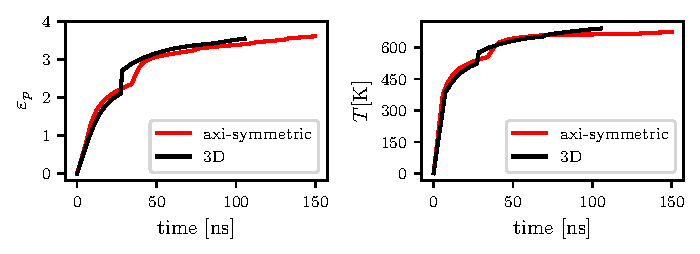
\includegraphics{cold-spray-plots}
  \caption{A PDF figure of which the font nearly matches the text font: 
  evolution of plastic strain $\varepsilon_p$ and temperature $T$ in time. Symbols, if any, in figures should be typeset with \LaTeX.  Be thourghful about colour blindness that affects around 8\% of men, particularly an inability to distinguish red and green. \texttt{matplotlib} can be colour-blind appropriate,  see line 29 of \cref{snippet_matplotlib}.}
  \label{fig:cold-spray-plot}
\end{figure}

\begin{figure}[!h]
  \centering
  %% Creator: Matplotlib, PGF backend
%%
%% To include the figure in your LaTeX document, write
%%   \input{<filename>.pgf}
%%
%% Make sure the required packages are loaded in your preamble
%%   \usepackage{pgf}
%%
%% Figures using additional raster images can only be included by \input if
%% they are in the same directory as the main LaTeX file. For loading figures
%% from other directories you can use the `import` package
%%   \usepackage{import}
%% and then include the figures with
%%   \import{<path to file>}{<filename>.pgf}
%%
%% Matplotlib used the following preamble
%%   \usepackage[utf8x]{inputenc}
%%   \usepackage[T1]{fontenc}
%%   \newcommand{\vect}[1]{#1}
%%
\begingroup%
\makeatletter%
\begin{pgfpicture}%
\pgfpathrectangle{\pgfpointorigin}{\pgfqpoint{6.375716in}{2.328394in}}%
\pgfusepath{use as bounding box, clip}%
\begin{pgfscope}%
\pgfsetbuttcap%
\pgfsetmiterjoin%
\definecolor{currentfill}{rgb}{1.000000,1.000000,1.000000}%
\pgfsetfillcolor{currentfill}%
\pgfsetlinewidth{0.000000pt}%
\definecolor{currentstroke}{rgb}{1.000000,1.000000,1.000000}%
\pgfsetstrokecolor{currentstroke}%
\pgfsetdash{}{0pt}%
\pgfpathmoveto{\pgfqpoint{0.000000in}{0.000000in}}%
\pgfpathlineto{\pgfqpoint{6.375716in}{0.000000in}}%
\pgfpathlineto{\pgfqpoint{6.375716in}{2.328394in}}%
\pgfpathlineto{\pgfqpoint{0.000000in}{2.328394in}}%
\pgfpathclose%
\pgfusepath{fill}%
\end{pgfscope}%
\begin{pgfscope}%
\pgfsetbuttcap%
\pgfsetmiterjoin%
\definecolor{currentfill}{rgb}{1.000000,1.000000,1.000000}%
\pgfsetfillcolor{currentfill}%
\pgfsetlinewidth{0.000000pt}%
\definecolor{currentstroke}{rgb}{0.000000,0.000000,0.000000}%
\pgfsetstrokecolor{currentstroke}%
\pgfsetstrokeopacity{0.000000}%
\pgfsetdash{}{0pt}%
\pgfpathmoveto{\pgfqpoint{0.434462in}{0.489757in}}%
\pgfpathlineto{\pgfqpoint{3.045729in}{0.489757in}}%
\pgfpathlineto{\pgfqpoint{3.045729in}{2.190131in}}%
\pgfpathlineto{\pgfqpoint{0.434462in}{2.190131in}}%
\pgfpathclose%
\pgfusepath{fill}%
\end{pgfscope}%
\begin{pgfscope}%
\pgfsetbuttcap%
\pgfsetroundjoin%
\definecolor{currentfill}{rgb}{0.000000,0.000000,0.000000}%
\pgfsetfillcolor{currentfill}%
\pgfsetlinewidth{0.803000pt}%
\definecolor{currentstroke}{rgb}{0.000000,0.000000,0.000000}%
\pgfsetstrokecolor{currentstroke}%
\pgfsetdash{}{0pt}%
\pgfsys@defobject{currentmarker}{\pgfqpoint{0.000000in}{-0.048611in}}{\pgfqpoint{0.000000in}{0.000000in}}{%
\pgfpathmoveto{\pgfqpoint{0.000000in}{0.000000in}}%
\pgfpathlineto{\pgfqpoint{0.000000in}{-0.048611in}}%
\pgfusepath{stroke,fill}%
}%
\begin{pgfscope}%
\pgfsys@transformshift{0.553156in}{0.489757in}%
\pgfsys@useobject{currentmarker}{}%
\end{pgfscope}%
\end{pgfscope}%
\begin{pgfscope}%
\definecolor{textcolor}{rgb}{0.000000,0.000000,0.000000}%
\pgfsetstrokecolor{textcolor}%
\pgfsetfillcolor{textcolor}%
\pgftext[x=0.553156in,y=0.392535in,,top]{\color{textcolor}\rmfamily\fontsize{8.000000}{9.600000}\selectfont \(\displaystyle 0\)}%
\end{pgfscope}%
\begin{pgfscope}%
\pgfsetbuttcap%
\pgfsetroundjoin%
\definecolor{currentfill}{rgb}{0.000000,0.000000,0.000000}%
\pgfsetfillcolor{currentfill}%
\pgfsetlinewidth{0.803000pt}%
\definecolor{currentstroke}{rgb}{0.000000,0.000000,0.000000}%
\pgfsetstrokecolor{currentstroke}%
\pgfsetdash{}{0pt}%
\pgfsys@defobject{currentmarker}{\pgfqpoint{0.000000in}{-0.048611in}}{\pgfqpoint{0.000000in}{0.000000in}}{%
\pgfpathmoveto{\pgfqpoint{0.000000in}{0.000000in}}%
\pgfpathlineto{\pgfqpoint{0.000000in}{-0.048611in}}%
\pgfusepath{stroke,fill}%
}%
\begin{pgfscope}%
\pgfsys@transformshift{0.948881in}{0.489757in}%
\pgfsys@useobject{currentmarker}{}%
\end{pgfscope}%
\end{pgfscope}%
\begin{pgfscope}%
\definecolor{textcolor}{rgb}{0.000000,0.000000,0.000000}%
\pgfsetstrokecolor{textcolor}%
\pgfsetfillcolor{textcolor}%
\pgftext[x=0.948881in,y=0.392535in,,top]{\color{textcolor}\rmfamily\fontsize{8.000000}{9.600000}\selectfont \(\displaystyle 25\)}%
\end{pgfscope}%
\begin{pgfscope}%
\pgfsetbuttcap%
\pgfsetroundjoin%
\definecolor{currentfill}{rgb}{0.000000,0.000000,0.000000}%
\pgfsetfillcolor{currentfill}%
\pgfsetlinewidth{0.803000pt}%
\definecolor{currentstroke}{rgb}{0.000000,0.000000,0.000000}%
\pgfsetstrokecolor{currentstroke}%
\pgfsetdash{}{0pt}%
\pgfsys@defobject{currentmarker}{\pgfqpoint{0.000000in}{-0.048611in}}{\pgfqpoint{0.000000in}{0.000000in}}{%
\pgfpathmoveto{\pgfqpoint{0.000000in}{0.000000in}}%
\pgfpathlineto{\pgfqpoint{0.000000in}{-0.048611in}}%
\pgfusepath{stroke,fill}%
}%
\begin{pgfscope}%
\pgfsys@transformshift{1.344607in}{0.489757in}%
\pgfsys@useobject{currentmarker}{}%
\end{pgfscope}%
\end{pgfscope}%
\begin{pgfscope}%
\definecolor{textcolor}{rgb}{0.000000,0.000000,0.000000}%
\pgfsetstrokecolor{textcolor}%
\pgfsetfillcolor{textcolor}%
\pgftext[x=1.344607in,y=0.392535in,,top]{\color{textcolor}\rmfamily\fontsize{8.000000}{9.600000}\selectfont \(\displaystyle 50\)}%
\end{pgfscope}%
\begin{pgfscope}%
\pgfsetbuttcap%
\pgfsetroundjoin%
\definecolor{currentfill}{rgb}{0.000000,0.000000,0.000000}%
\pgfsetfillcolor{currentfill}%
\pgfsetlinewidth{0.803000pt}%
\definecolor{currentstroke}{rgb}{0.000000,0.000000,0.000000}%
\pgfsetstrokecolor{currentstroke}%
\pgfsetdash{}{0pt}%
\pgfsys@defobject{currentmarker}{\pgfqpoint{0.000000in}{-0.048611in}}{\pgfqpoint{0.000000in}{0.000000in}}{%
\pgfpathmoveto{\pgfqpoint{0.000000in}{0.000000in}}%
\pgfpathlineto{\pgfqpoint{0.000000in}{-0.048611in}}%
\pgfusepath{stroke,fill}%
}%
\begin{pgfscope}%
\pgfsys@transformshift{1.740333in}{0.489757in}%
\pgfsys@useobject{currentmarker}{}%
\end{pgfscope}%
\end{pgfscope}%
\begin{pgfscope}%
\definecolor{textcolor}{rgb}{0.000000,0.000000,0.000000}%
\pgfsetstrokecolor{textcolor}%
\pgfsetfillcolor{textcolor}%
\pgftext[x=1.740333in,y=0.392535in,,top]{\color{textcolor}\rmfamily\fontsize{8.000000}{9.600000}\selectfont \(\displaystyle 75\)}%
\end{pgfscope}%
\begin{pgfscope}%
\pgfsetbuttcap%
\pgfsetroundjoin%
\definecolor{currentfill}{rgb}{0.000000,0.000000,0.000000}%
\pgfsetfillcolor{currentfill}%
\pgfsetlinewidth{0.803000pt}%
\definecolor{currentstroke}{rgb}{0.000000,0.000000,0.000000}%
\pgfsetstrokecolor{currentstroke}%
\pgfsetdash{}{0pt}%
\pgfsys@defobject{currentmarker}{\pgfqpoint{0.000000in}{-0.048611in}}{\pgfqpoint{0.000000in}{0.000000in}}{%
\pgfpathmoveto{\pgfqpoint{0.000000in}{0.000000in}}%
\pgfpathlineto{\pgfqpoint{0.000000in}{-0.048611in}}%
\pgfusepath{stroke,fill}%
}%
\begin{pgfscope}%
\pgfsys@transformshift{2.136059in}{0.489757in}%
\pgfsys@useobject{currentmarker}{}%
\end{pgfscope}%
\end{pgfscope}%
\begin{pgfscope}%
\definecolor{textcolor}{rgb}{0.000000,0.000000,0.000000}%
\pgfsetstrokecolor{textcolor}%
\pgfsetfillcolor{textcolor}%
\pgftext[x=2.136059in,y=0.392535in,,top]{\color{textcolor}\rmfamily\fontsize{8.000000}{9.600000}\selectfont \(\displaystyle 100\)}%
\end{pgfscope}%
\begin{pgfscope}%
\pgfsetbuttcap%
\pgfsetroundjoin%
\definecolor{currentfill}{rgb}{0.000000,0.000000,0.000000}%
\pgfsetfillcolor{currentfill}%
\pgfsetlinewidth{0.803000pt}%
\definecolor{currentstroke}{rgb}{0.000000,0.000000,0.000000}%
\pgfsetstrokecolor{currentstroke}%
\pgfsetdash{}{0pt}%
\pgfsys@defobject{currentmarker}{\pgfqpoint{0.000000in}{-0.048611in}}{\pgfqpoint{0.000000in}{0.000000in}}{%
\pgfpathmoveto{\pgfqpoint{0.000000in}{0.000000in}}%
\pgfpathlineto{\pgfqpoint{0.000000in}{-0.048611in}}%
\pgfusepath{stroke,fill}%
}%
\begin{pgfscope}%
\pgfsys@transformshift{2.531785in}{0.489757in}%
\pgfsys@useobject{currentmarker}{}%
\end{pgfscope}%
\end{pgfscope}%
\begin{pgfscope}%
\definecolor{textcolor}{rgb}{0.000000,0.000000,0.000000}%
\pgfsetstrokecolor{textcolor}%
\pgfsetfillcolor{textcolor}%
\pgftext[x=2.531785in,y=0.392535in,,top]{\color{textcolor}\rmfamily\fontsize{8.000000}{9.600000}\selectfont \(\displaystyle 125\)}%
\end{pgfscope}%
\begin{pgfscope}%
\pgfsetbuttcap%
\pgfsetroundjoin%
\definecolor{currentfill}{rgb}{0.000000,0.000000,0.000000}%
\pgfsetfillcolor{currentfill}%
\pgfsetlinewidth{0.803000pt}%
\definecolor{currentstroke}{rgb}{0.000000,0.000000,0.000000}%
\pgfsetstrokecolor{currentstroke}%
\pgfsetdash{}{0pt}%
\pgfsys@defobject{currentmarker}{\pgfqpoint{0.000000in}{-0.048611in}}{\pgfqpoint{0.000000in}{0.000000in}}{%
\pgfpathmoveto{\pgfqpoint{0.000000in}{0.000000in}}%
\pgfpathlineto{\pgfqpoint{0.000000in}{-0.048611in}}%
\pgfusepath{stroke,fill}%
}%
\begin{pgfscope}%
\pgfsys@transformshift{2.927510in}{0.489757in}%
\pgfsys@useobject{currentmarker}{}%
\end{pgfscope}%
\end{pgfscope}%
\begin{pgfscope}%
\definecolor{textcolor}{rgb}{0.000000,0.000000,0.000000}%
\pgfsetstrokecolor{textcolor}%
\pgfsetfillcolor{textcolor}%
\pgftext[x=2.927510in,y=0.392535in,,top]{\color{textcolor}\rmfamily\fontsize{8.000000}{9.600000}\selectfont \(\displaystyle 150\)}%
\end{pgfscope}%
\begin{pgfscope}%
\definecolor{textcolor}{rgb}{0.000000,0.000000,0.000000}%
\pgfsetstrokecolor{textcolor}%
\pgfsetfillcolor{textcolor}%
\pgftext[x=1.740096in,y=0.238855in,,top]{\color{textcolor}\rmfamily\fontsize{10.000000}{12.000000}\selectfont time [ns]}%
\end{pgfscope}%
\begin{pgfscope}%
\pgfsetbuttcap%
\pgfsetroundjoin%
\definecolor{currentfill}{rgb}{0.000000,0.000000,0.000000}%
\pgfsetfillcolor{currentfill}%
\pgfsetlinewidth{0.803000pt}%
\definecolor{currentstroke}{rgb}{0.000000,0.000000,0.000000}%
\pgfsetstrokecolor{currentstroke}%
\pgfsetdash{}{0pt}%
\pgfsys@defobject{currentmarker}{\pgfqpoint{-0.048611in}{0.000000in}}{\pgfqpoint{0.000000in}{0.000000in}}{%
\pgfpathmoveto{\pgfqpoint{0.000000in}{0.000000in}}%
\pgfpathlineto{\pgfqpoint{-0.048611in}{0.000000in}}%
\pgfusepath{stroke,fill}%
}%
\begin{pgfscope}%
\pgfsys@transformshift{0.434462in}{0.563078in}%
\pgfsys@useobject{currentmarker}{}%
\end{pgfscope}%
\end{pgfscope}%
\begin{pgfscope}%
\definecolor{textcolor}{rgb}{0.000000,0.000000,0.000000}%
\pgfsetstrokecolor{textcolor}%
\pgfsetfillcolor{textcolor}%
\pgftext[x=0.278211in,y=0.524816in,left,base]{\color{textcolor}\rmfamily\fontsize{8.000000}{9.600000}\selectfont \(\displaystyle 0\)}%
\end{pgfscope}%
\begin{pgfscope}%
\pgfsetbuttcap%
\pgfsetroundjoin%
\definecolor{currentfill}{rgb}{0.000000,0.000000,0.000000}%
\pgfsetfillcolor{currentfill}%
\pgfsetlinewidth{0.803000pt}%
\definecolor{currentstroke}{rgb}{0.000000,0.000000,0.000000}%
\pgfsetstrokecolor{currentstroke}%
\pgfsetdash{}{0pt}%
\pgfsys@defobject{currentmarker}{\pgfqpoint{-0.048611in}{0.000000in}}{\pgfqpoint{0.000000in}{0.000000in}}{%
\pgfpathmoveto{\pgfqpoint{0.000000in}{0.000000in}}%
\pgfpathlineto{\pgfqpoint{-0.048611in}{0.000000in}}%
\pgfusepath{stroke,fill}%
}%
\begin{pgfscope}%
\pgfsys@transformshift{0.434462in}{0.969841in}%
\pgfsys@useobject{currentmarker}{}%
\end{pgfscope}%
\end{pgfscope}%
\begin{pgfscope}%
\definecolor{textcolor}{rgb}{0.000000,0.000000,0.000000}%
\pgfsetstrokecolor{textcolor}%
\pgfsetfillcolor{textcolor}%
\pgftext[x=0.278211in,y=0.931579in,left,base]{\color{textcolor}\rmfamily\fontsize{8.000000}{9.600000}\selectfont \(\displaystyle 1\)}%
\end{pgfscope}%
\begin{pgfscope}%
\pgfsetbuttcap%
\pgfsetroundjoin%
\definecolor{currentfill}{rgb}{0.000000,0.000000,0.000000}%
\pgfsetfillcolor{currentfill}%
\pgfsetlinewidth{0.803000pt}%
\definecolor{currentstroke}{rgb}{0.000000,0.000000,0.000000}%
\pgfsetstrokecolor{currentstroke}%
\pgfsetdash{}{0pt}%
\pgfsys@defobject{currentmarker}{\pgfqpoint{-0.048611in}{0.000000in}}{\pgfqpoint{0.000000in}{0.000000in}}{%
\pgfpathmoveto{\pgfqpoint{0.000000in}{0.000000in}}%
\pgfpathlineto{\pgfqpoint{-0.048611in}{0.000000in}}%
\pgfusepath{stroke,fill}%
}%
\begin{pgfscope}%
\pgfsys@transformshift{0.434462in}{1.376605in}%
\pgfsys@useobject{currentmarker}{}%
\end{pgfscope}%
\end{pgfscope}%
\begin{pgfscope}%
\definecolor{textcolor}{rgb}{0.000000,0.000000,0.000000}%
\pgfsetstrokecolor{textcolor}%
\pgfsetfillcolor{textcolor}%
\pgftext[x=0.278211in,y=1.338342in,left,base]{\color{textcolor}\rmfamily\fontsize{8.000000}{9.600000}\selectfont \(\displaystyle 2\)}%
\end{pgfscope}%
\begin{pgfscope}%
\pgfsetbuttcap%
\pgfsetroundjoin%
\definecolor{currentfill}{rgb}{0.000000,0.000000,0.000000}%
\pgfsetfillcolor{currentfill}%
\pgfsetlinewidth{0.803000pt}%
\definecolor{currentstroke}{rgb}{0.000000,0.000000,0.000000}%
\pgfsetstrokecolor{currentstroke}%
\pgfsetdash{}{0pt}%
\pgfsys@defobject{currentmarker}{\pgfqpoint{-0.048611in}{0.000000in}}{\pgfqpoint{0.000000in}{0.000000in}}{%
\pgfpathmoveto{\pgfqpoint{0.000000in}{0.000000in}}%
\pgfpathlineto{\pgfqpoint{-0.048611in}{0.000000in}}%
\pgfusepath{stroke,fill}%
}%
\begin{pgfscope}%
\pgfsys@transformshift{0.434462in}{1.783368in}%
\pgfsys@useobject{currentmarker}{}%
\end{pgfscope}%
\end{pgfscope}%
\begin{pgfscope}%
\definecolor{textcolor}{rgb}{0.000000,0.000000,0.000000}%
\pgfsetstrokecolor{textcolor}%
\pgfsetfillcolor{textcolor}%
\pgftext[x=0.278211in,y=1.745106in,left,base]{\color{textcolor}\rmfamily\fontsize{8.000000}{9.600000}\selectfont \(\displaystyle 3\)}%
\end{pgfscope}%
\begin{pgfscope}%
\pgfsetbuttcap%
\pgfsetroundjoin%
\definecolor{currentfill}{rgb}{0.000000,0.000000,0.000000}%
\pgfsetfillcolor{currentfill}%
\pgfsetlinewidth{0.803000pt}%
\definecolor{currentstroke}{rgb}{0.000000,0.000000,0.000000}%
\pgfsetstrokecolor{currentstroke}%
\pgfsetdash{}{0pt}%
\pgfsys@defobject{currentmarker}{\pgfqpoint{-0.048611in}{0.000000in}}{\pgfqpoint{0.000000in}{0.000000in}}{%
\pgfpathmoveto{\pgfqpoint{0.000000in}{0.000000in}}%
\pgfpathlineto{\pgfqpoint{-0.048611in}{0.000000in}}%
\pgfusepath{stroke,fill}%
}%
\begin{pgfscope}%
\pgfsys@transformshift{0.434462in}{2.190131in}%
\pgfsys@useobject{currentmarker}{}%
\end{pgfscope}%
\end{pgfscope}%
\begin{pgfscope}%
\definecolor{textcolor}{rgb}{0.000000,0.000000,0.000000}%
\pgfsetstrokecolor{textcolor}%
\pgfsetfillcolor{textcolor}%
\pgftext[x=0.278211in,y=2.151869in,left,base]{\color{textcolor}\rmfamily\fontsize{8.000000}{9.600000}\selectfont \(\displaystyle 4\)}%
\end{pgfscope}%
\begin{pgfscope}%
\definecolor{textcolor}{rgb}{0.000000,0.000000,0.000000}%
\pgfsetstrokecolor{textcolor}%
\pgfsetfillcolor{textcolor}%
\pgftext[x=0.222655in,y=1.339944in,,bottom,rotate=90.000000]{\color{textcolor}\rmfamily\fontsize{10.000000}{12.000000}\selectfont \(\displaystyle \varepsilon_p\)}%
\end{pgfscope}%
\begin{pgfscope}%
\pgfpathrectangle{\pgfqpoint{0.434462in}{0.489757in}}{\pgfqpoint{2.611268in}{1.700374in}}%
\pgfusepath{clip}%
\pgfsetrectcap%
\pgfsetroundjoin%
\pgfsetlinewidth{1.505625pt}%
\definecolor{currentstroke}{rgb}{1.000000,0.000000,0.000000}%
\pgfsetstrokecolor{currentstroke}%
\pgfsetdash{}{0pt}%
\pgfpathmoveto{\pgfqpoint{0.553156in}{0.563078in}}%
\pgfpathlineto{\pgfqpoint{0.644136in}{0.898446in}}%
\pgfpathlineto{\pgfqpoint{0.677856in}{1.049453in}}%
\pgfpathlineto{\pgfqpoint{0.701275in}{1.128621in}}%
\pgfpathlineto{\pgfqpoint{0.720070in}{1.178198in}}%
\pgfpathlineto{\pgfqpoint{0.750463in}{1.247038in}}%
\pgfpathlineto{\pgfqpoint{0.763527in}{1.269512in}}%
\pgfpathlineto{\pgfqpoint{0.787471in}{1.301349in}}%
\pgfpathlineto{\pgfqpoint{0.819226in}{1.343112in}}%
\pgfpathlineto{\pgfqpoint{0.838567in}{1.361445in}}%
\pgfpathlineto{\pgfqpoint{0.899727in}{1.413807in}}%
\pgfpathlineto{\pgfqpoint{0.923829in}{1.429057in}}%
\pgfpathlineto{\pgfqpoint{0.946966in}{1.443696in}}%
\pgfpathlineto{\pgfqpoint{0.961875in}{1.454223in}}%
\pgfpathlineto{\pgfqpoint{0.983819in}{1.465991in}}%
\pgfpathlineto{\pgfqpoint{1.019222in}{1.483819in}}%
\pgfpathlineto{\pgfqpoint{1.032951in}{1.491572in}}%
\pgfpathlineto{\pgfqpoint{1.053315in}{1.500452in}}%
\pgfpathlineto{\pgfqpoint{1.086542in}{1.514200in}}%
\pgfpathlineto{\pgfqpoint{1.093049in}{1.517463in}}%
\pgfpathlineto{\pgfqpoint{1.099529in}{1.524715in}}%
\pgfpathlineto{\pgfqpoint{1.125278in}{1.594898in}}%
\pgfpathlineto{\pgfqpoint{1.144395in}{1.640806in}}%
\pgfpathlineto{\pgfqpoint{1.163208in}{1.678936in}}%
\pgfpathlineto{\pgfqpoint{1.181844in}{1.710216in}}%
\pgfpathlineto{\pgfqpoint{1.194230in}{1.728805in}}%
\pgfpathlineto{\pgfqpoint{1.206584in}{1.743741in}}%
\pgfpathlineto{\pgfqpoint{1.218857in}{1.753093in}}%
\pgfpathlineto{\pgfqpoint{1.254602in}{1.776233in}}%
\pgfpathlineto{\pgfqpoint{1.272082in}{1.786492in}}%
\pgfpathlineto{\pgfqpoint{1.289316in}{1.793944in}}%
\pgfpathlineto{\pgfqpoint{1.322880in}{1.804577in}}%
\pgfpathlineto{\pgfqpoint{1.361164in}{1.814729in}}%
\pgfpathlineto{\pgfqpoint{1.461503in}{1.836996in}}%
\pgfpathlineto{\pgfqpoint{1.523974in}{1.848283in}}%
\pgfpathlineto{\pgfqpoint{1.581436in}{1.856642in}}%
\pgfpathlineto{\pgfqpoint{1.655624in}{1.867027in}}%
\pgfpathlineto{\pgfqpoint{1.704159in}{1.877143in}}%
\pgfpathlineto{\pgfqpoint{1.720447in}{1.882065in}}%
\pgfpathlineto{\pgfqpoint{1.731353in}{1.887589in}}%
\pgfpathlineto{\pgfqpoint{1.736822in}{1.894923in}}%
\pgfpathlineto{\pgfqpoint{1.792102in}{1.902875in}}%
\pgfpathlineto{\pgfqpoint{1.888103in}{1.914395in}}%
\pgfpathlineto{\pgfqpoint{1.974797in}{1.922213in}}%
\pgfpathlineto{\pgfqpoint{2.105240in}{1.933289in}}%
\pgfpathlineto{\pgfqpoint{2.269941in}{1.950580in}}%
\pgfpathlineto{\pgfqpoint{2.307076in}{1.956071in}}%
\pgfpathlineto{\pgfqpoint{2.325738in}{1.960619in}}%
\pgfpathlineto{\pgfqpoint{2.338211in}{1.967221in}}%
\pgfpathlineto{\pgfqpoint{2.438726in}{1.974868in}}%
\pgfpathlineto{\pgfqpoint{2.598203in}{1.991277in}}%
\pgfpathlineto{\pgfqpoint{2.630368in}{1.996601in}}%
\pgfpathlineto{\pgfqpoint{2.643253in}{2.001076in}}%
\pgfpathlineto{\pgfqpoint{2.649711in}{2.006563in}}%
\pgfpathlineto{\pgfqpoint{2.830542in}{2.022651in}}%
\pgfpathlineto{\pgfqpoint{2.927035in}{2.029496in}}%
\pgfpathlineto{\pgfqpoint{2.927035in}{2.029496in}}%
\pgfusepath{stroke}%
\end{pgfscope}%
\begin{pgfscope}%
\pgfsetrectcap%
\pgfsetmiterjoin%
\pgfsetlinewidth{0.803000pt}%
\definecolor{currentstroke}{rgb}{0.000000,0.000000,0.000000}%
\pgfsetstrokecolor{currentstroke}%
\pgfsetdash{}{0pt}%
\pgfpathmoveto{\pgfqpoint{0.434462in}{0.489757in}}%
\pgfpathlineto{\pgfqpoint{0.434462in}{2.190131in}}%
\pgfusepath{stroke}%
\end{pgfscope}%
\begin{pgfscope}%
\pgfsetrectcap%
\pgfsetmiterjoin%
\pgfsetlinewidth{0.803000pt}%
\definecolor{currentstroke}{rgb}{0.000000,0.000000,0.000000}%
\pgfsetstrokecolor{currentstroke}%
\pgfsetdash{}{0pt}%
\pgfpathmoveto{\pgfqpoint{3.045729in}{0.489757in}}%
\pgfpathlineto{\pgfqpoint{3.045729in}{2.190131in}}%
\pgfusepath{stroke}%
\end{pgfscope}%
\begin{pgfscope}%
\pgfsetrectcap%
\pgfsetmiterjoin%
\pgfsetlinewidth{0.803000pt}%
\definecolor{currentstroke}{rgb}{0.000000,0.000000,0.000000}%
\pgfsetstrokecolor{currentstroke}%
\pgfsetdash{}{0pt}%
\pgfpathmoveto{\pgfqpoint{0.434462in}{0.489757in}}%
\pgfpathlineto{\pgfqpoint{3.045729in}{0.489757in}}%
\pgfusepath{stroke}%
\end{pgfscope}%
\begin{pgfscope}%
\pgfsetrectcap%
\pgfsetmiterjoin%
\pgfsetlinewidth{0.803000pt}%
\definecolor{currentstroke}{rgb}{0.000000,0.000000,0.000000}%
\pgfsetstrokecolor{currentstroke}%
\pgfsetdash{}{0pt}%
\pgfpathmoveto{\pgfqpoint{0.434462in}{2.190131in}}%
\pgfpathlineto{\pgfqpoint{3.045729in}{2.190131in}}%
\pgfusepath{stroke}%
\end{pgfscope}%
\begin{pgfscope}%
\pgfsetbuttcap%
\pgfsetmiterjoin%
\definecolor{currentfill}{rgb}{1.000000,1.000000,1.000000}%
\pgfsetfillcolor{currentfill}%
\pgfsetfillopacity{0.800000}%
\pgfsetlinewidth{1.003750pt}%
\definecolor{currentstroke}{rgb}{0.800000,0.800000,0.800000}%
\pgfsetstrokecolor{currentstroke}%
\pgfsetstrokeopacity{0.800000}%
\pgfsetdash{}{0pt}%
\pgfpathmoveto{\pgfqpoint{0.512239in}{1.946309in}}%
\pgfpathlineto{\pgfqpoint{1.596378in}{1.946309in}}%
\pgfpathquadraticcurveto{\pgfqpoint{1.618601in}{1.946309in}}{\pgfqpoint{1.618601in}{1.968532in}}%
\pgfpathlineto{\pgfqpoint{1.618601in}{2.112353in}}%
\pgfpathquadraticcurveto{\pgfqpoint{1.618601in}{2.134576in}}{\pgfqpoint{1.596378in}{2.134576in}}%
\pgfpathlineto{\pgfqpoint{0.512239in}{2.134576in}}%
\pgfpathquadraticcurveto{\pgfqpoint{0.490017in}{2.134576in}}{\pgfqpoint{0.490017in}{2.112353in}}%
\pgfpathlineto{\pgfqpoint{0.490017in}{1.968532in}}%
\pgfpathquadraticcurveto{\pgfqpoint{0.490017in}{1.946309in}}{\pgfqpoint{0.512239in}{1.946309in}}%
\pgfpathclose%
\pgfusepath{stroke,fill}%
\end{pgfscope}%
\begin{pgfscope}%
\pgfsetrectcap%
\pgfsetroundjoin%
\pgfsetlinewidth{1.505625pt}%
\definecolor{currentstroke}{rgb}{1.000000,0.000000,0.000000}%
\pgfsetstrokecolor{currentstroke}%
\pgfsetdash{}{0pt}%
\pgfpathmoveto{\pgfqpoint{0.534462in}{2.051242in}}%
\pgfpathlineto{\pgfqpoint{0.756684in}{2.051242in}}%
\pgfusepath{stroke}%
\end{pgfscope}%
\begin{pgfscope}%
\definecolor{textcolor}{rgb}{0.000000,0.000000,0.000000}%
\pgfsetstrokecolor{textcolor}%
\pgfsetfillcolor{textcolor}%
\pgftext[x=0.845573in,y=2.012353in,left,base]{\color{textcolor}\rmfamily\fontsize{8.000000}{9.600000}\selectfont axi-symmetric}%
\end{pgfscope}%
\begin{pgfscope}%
\pgfsetbuttcap%
\pgfsetmiterjoin%
\definecolor{currentfill}{rgb}{1.000000,1.000000,1.000000}%
\pgfsetfillcolor{currentfill}%
\pgfsetlinewidth{0.000000pt}%
\definecolor{currentstroke}{rgb}{0.000000,0.000000,0.000000}%
\pgfsetstrokecolor{currentstroke}%
\pgfsetstrokeopacity{0.000000}%
\pgfsetdash{}{0pt}%
\pgfpathmoveto{\pgfqpoint{3.664448in}{0.489757in}}%
\pgfpathlineto{\pgfqpoint{6.275716in}{0.489757in}}%
\pgfpathlineto{\pgfqpoint{6.275716in}{2.190131in}}%
\pgfpathlineto{\pgfqpoint{3.664448in}{2.190131in}}%
\pgfpathclose%
\pgfusepath{fill}%
\end{pgfscope}%
\begin{pgfscope}%
\pgfsetbuttcap%
\pgfsetroundjoin%
\definecolor{currentfill}{rgb}{0.000000,0.000000,0.000000}%
\pgfsetfillcolor{currentfill}%
\pgfsetlinewidth{0.803000pt}%
\definecolor{currentstroke}{rgb}{0.000000,0.000000,0.000000}%
\pgfsetstrokecolor{currentstroke}%
\pgfsetdash{}{0pt}%
\pgfsys@defobject{currentmarker}{\pgfqpoint{0.000000in}{-0.048611in}}{\pgfqpoint{0.000000in}{0.000000in}}{%
\pgfpathmoveto{\pgfqpoint{0.000000in}{0.000000in}}%
\pgfpathlineto{\pgfqpoint{0.000000in}{-0.048611in}}%
\pgfusepath{stroke,fill}%
}%
\begin{pgfscope}%
\pgfsys@transformshift{3.783142in}{0.489757in}%
\pgfsys@useobject{currentmarker}{}%
\end{pgfscope}%
\end{pgfscope}%
\begin{pgfscope}%
\definecolor{textcolor}{rgb}{0.000000,0.000000,0.000000}%
\pgfsetstrokecolor{textcolor}%
\pgfsetfillcolor{textcolor}%
\pgftext[x=3.783142in,y=0.392535in,,top]{\color{textcolor}\rmfamily\fontsize{8.000000}{9.600000}\selectfont \(\displaystyle 0\)}%
\end{pgfscope}%
\begin{pgfscope}%
\pgfsetbuttcap%
\pgfsetroundjoin%
\definecolor{currentfill}{rgb}{0.000000,0.000000,0.000000}%
\pgfsetfillcolor{currentfill}%
\pgfsetlinewidth{0.803000pt}%
\definecolor{currentstroke}{rgb}{0.000000,0.000000,0.000000}%
\pgfsetstrokecolor{currentstroke}%
\pgfsetdash{}{0pt}%
\pgfsys@defobject{currentmarker}{\pgfqpoint{0.000000in}{-0.048611in}}{\pgfqpoint{0.000000in}{0.000000in}}{%
\pgfpathmoveto{\pgfqpoint{0.000000in}{0.000000in}}%
\pgfpathlineto{\pgfqpoint{0.000000in}{-0.048611in}}%
\pgfusepath{stroke,fill}%
}%
\begin{pgfscope}%
\pgfsys@transformshift{4.178868in}{0.489757in}%
\pgfsys@useobject{currentmarker}{}%
\end{pgfscope}%
\end{pgfscope}%
\begin{pgfscope}%
\definecolor{textcolor}{rgb}{0.000000,0.000000,0.000000}%
\pgfsetstrokecolor{textcolor}%
\pgfsetfillcolor{textcolor}%
\pgftext[x=4.178868in,y=0.392535in,,top]{\color{textcolor}\rmfamily\fontsize{8.000000}{9.600000}\selectfont \(\displaystyle 25\)}%
\end{pgfscope}%
\begin{pgfscope}%
\pgfsetbuttcap%
\pgfsetroundjoin%
\definecolor{currentfill}{rgb}{0.000000,0.000000,0.000000}%
\pgfsetfillcolor{currentfill}%
\pgfsetlinewidth{0.803000pt}%
\definecolor{currentstroke}{rgb}{0.000000,0.000000,0.000000}%
\pgfsetstrokecolor{currentstroke}%
\pgfsetdash{}{0pt}%
\pgfsys@defobject{currentmarker}{\pgfqpoint{0.000000in}{-0.048611in}}{\pgfqpoint{0.000000in}{0.000000in}}{%
\pgfpathmoveto{\pgfqpoint{0.000000in}{0.000000in}}%
\pgfpathlineto{\pgfqpoint{0.000000in}{-0.048611in}}%
\pgfusepath{stroke,fill}%
}%
\begin{pgfscope}%
\pgfsys@transformshift{4.574594in}{0.489757in}%
\pgfsys@useobject{currentmarker}{}%
\end{pgfscope}%
\end{pgfscope}%
\begin{pgfscope}%
\definecolor{textcolor}{rgb}{0.000000,0.000000,0.000000}%
\pgfsetstrokecolor{textcolor}%
\pgfsetfillcolor{textcolor}%
\pgftext[x=4.574594in,y=0.392535in,,top]{\color{textcolor}\rmfamily\fontsize{8.000000}{9.600000}\selectfont \(\displaystyle 50\)}%
\end{pgfscope}%
\begin{pgfscope}%
\pgfsetbuttcap%
\pgfsetroundjoin%
\definecolor{currentfill}{rgb}{0.000000,0.000000,0.000000}%
\pgfsetfillcolor{currentfill}%
\pgfsetlinewidth{0.803000pt}%
\definecolor{currentstroke}{rgb}{0.000000,0.000000,0.000000}%
\pgfsetstrokecolor{currentstroke}%
\pgfsetdash{}{0pt}%
\pgfsys@defobject{currentmarker}{\pgfqpoint{0.000000in}{-0.048611in}}{\pgfqpoint{0.000000in}{0.000000in}}{%
\pgfpathmoveto{\pgfqpoint{0.000000in}{0.000000in}}%
\pgfpathlineto{\pgfqpoint{0.000000in}{-0.048611in}}%
\pgfusepath{stroke,fill}%
}%
\begin{pgfscope}%
\pgfsys@transformshift{4.970320in}{0.489757in}%
\pgfsys@useobject{currentmarker}{}%
\end{pgfscope}%
\end{pgfscope}%
\begin{pgfscope}%
\definecolor{textcolor}{rgb}{0.000000,0.000000,0.000000}%
\pgfsetstrokecolor{textcolor}%
\pgfsetfillcolor{textcolor}%
\pgftext[x=4.970320in,y=0.392535in,,top]{\color{textcolor}\rmfamily\fontsize{8.000000}{9.600000}\selectfont \(\displaystyle 75\)}%
\end{pgfscope}%
\begin{pgfscope}%
\pgfsetbuttcap%
\pgfsetroundjoin%
\definecolor{currentfill}{rgb}{0.000000,0.000000,0.000000}%
\pgfsetfillcolor{currentfill}%
\pgfsetlinewidth{0.803000pt}%
\definecolor{currentstroke}{rgb}{0.000000,0.000000,0.000000}%
\pgfsetstrokecolor{currentstroke}%
\pgfsetdash{}{0pt}%
\pgfsys@defobject{currentmarker}{\pgfqpoint{0.000000in}{-0.048611in}}{\pgfqpoint{0.000000in}{0.000000in}}{%
\pgfpathmoveto{\pgfqpoint{0.000000in}{0.000000in}}%
\pgfpathlineto{\pgfqpoint{0.000000in}{-0.048611in}}%
\pgfusepath{stroke,fill}%
}%
\begin{pgfscope}%
\pgfsys@transformshift{5.366045in}{0.489757in}%
\pgfsys@useobject{currentmarker}{}%
\end{pgfscope}%
\end{pgfscope}%
\begin{pgfscope}%
\definecolor{textcolor}{rgb}{0.000000,0.000000,0.000000}%
\pgfsetstrokecolor{textcolor}%
\pgfsetfillcolor{textcolor}%
\pgftext[x=5.366045in,y=0.392535in,,top]{\color{textcolor}\rmfamily\fontsize{8.000000}{9.600000}\selectfont \(\displaystyle 100\)}%
\end{pgfscope}%
\begin{pgfscope}%
\pgfsetbuttcap%
\pgfsetroundjoin%
\definecolor{currentfill}{rgb}{0.000000,0.000000,0.000000}%
\pgfsetfillcolor{currentfill}%
\pgfsetlinewidth{0.803000pt}%
\definecolor{currentstroke}{rgb}{0.000000,0.000000,0.000000}%
\pgfsetstrokecolor{currentstroke}%
\pgfsetdash{}{0pt}%
\pgfsys@defobject{currentmarker}{\pgfqpoint{0.000000in}{-0.048611in}}{\pgfqpoint{0.000000in}{0.000000in}}{%
\pgfpathmoveto{\pgfqpoint{0.000000in}{0.000000in}}%
\pgfpathlineto{\pgfqpoint{0.000000in}{-0.048611in}}%
\pgfusepath{stroke,fill}%
}%
\begin{pgfscope}%
\pgfsys@transformshift{5.761771in}{0.489757in}%
\pgfsys@useobject{currentmarker}{}%
\end{pgfscope}%
\end{pgfscope}%
\begin{pgfscope}%
\definecolor{textcolor}{rgb}{0.000000,0.000000,0.000000}%
\pgfsetstrokecolor{textcolor}%
\pgfsetfillcolor{textcolor}%
\pgftext[x=5.761771in,y=0.392535in,,top]{\color{textcolor}\rmfamily\fontsize{8.000000}{9.600000}\selectfont \(\displaystyle 125\)}%
\end{pgfscope}%
\begin{pgfscope}%
\pgfsetbuttcap%
\pgfsetroundjoin%
\definecolor{currentfill}{rgb}{0.000000,0.000000,0.000000}%
\pgfsetfillcolor{currentfill}%
\pgfsetlinewidth{0.803000pt}%
\definecolor{currentstroke}{rgb}{0.000000,0.000000,0.000000}%
\pgfsetstrokecolor{currentstroke}%
\pgfsetdash{}{0pt}%
\pgfsys@defobject{currentmarker}{\pgfqpoint{0.000000in}{-0.048611in}}{\pgfqpoint{0.000000in}{0.000000in}}{%
\pgfpathmoveto{\pgfqpoint{0.000000in}{0.000000in}}%
\pgfpathlineto{\pgfqpoint{0.000000in}{-0.048611in}}%
\pgfusepath{stroke,fill}%
}%
\begin{pgfscope}%
\pgfsys@transformshift{6.157497in}{0.489757in}%
\pgfsys@useobject{currentmarker}{}%
\end{pgfscope}%
\end{pgfscope}%
\begin{pgfscope}%
\definecolor{textcolor}{rgb}{0.000000,0.000000,0.000000}%
\pgfsetstrokecolor{textcolor}%
\pgfsetfillcolor{textcolor}%
\pgftext[x=6.157497in,y=0.392535in,,top]{\color{textcolor}\rmfamily\fontsize{8.000000}{9.600000}\selectfont \(\displaystyle 150\)}%
\end{pgfscope}%
\begin{pgfscope}%
\definecolor{textcolor}{rgb}{0.000000,0.000000,0.000000}%
\pgfsetstrokecolor{textcolor}%
\pgfsetfillcolor{textcolor}%
\pgftext[x=4.970082in,y=0.238855in,,top]{\color{textcolor}\rmfamily\fontsize{10.000000}{12.000000}\selectfont time [ns]}%
\end{pgfscope}%
\begin{pgfscope}%
\pgfsetbuttcap%
\pgfsetroundjoin%
\definecolor{currentfill}{rgb}{0.000000,0.000000,0.000000}%
\pgfsetfillcolor{currentfill}%
\pgfsetlinewidth{0.803000pt}%
\definecolor{currentstroke}{rgb}{0.000000,0.000000,0.000000}%
\pgfsetstrokecolor{currentstroke}%
\pgfsetdash{}{0pt}%
\pgfsys@defobject{currentmarker}{\pgfqpoint{-0.048611in}{0.000000in}}{\pgfqpoint{0.000000in}{0.000000in}}{%
\pgfpathmoveto{\pgfqpoint{0.000000in}{0.000000in}}%
\pgfpathlineto{\pgfqpoint{-0.048611in}{0.000000in}}%
\pgfusepath{stroke,fill}%
}%
\begin{pgfscope}%
\pgfsys@transformshift{3.664448in}{0.567047in}%
\pgfsys@useobject{currentmarker}{}%
\end{pgfscope}%
\end{pgfscope}%
\begin{pgfscope}%
\definecolor{textcolor}{rgb}{0.000000,0.000000,0.000000}%
\pgfsetstrokecolor{textcolor}%
\pgfsetfillcolor{textcolor}%
\pgftext[x=3.508197in,y=0.528785in,left,base]{\color{textcolor}\rmfamily\fontsize{8.000000}{9.600000}\selectfont \(\displaystyle 0\)}%
\end{pgfscope}%
\begin{pgfscope}%
\pgfsetbuttcap%
\pgfsetroundjoin%
\definecolor{currentfill}{rgb}{0.000000,0.000000,0.000000}%
\pgfsetfillcolor{currentfill}%
\pgfsetlinewidth{0.803000pt}%
\definecolor{currentstroke}{rgb}{0.000000,0.000000,0.000000}%
\pgfsetstrokecolor{currentstroke}%
\pgfsetdash{}{0pt}%
\pgfsys@defobject{currentmarker}{\pgfqpoint{-0.048611in}{0.000000in}}{\pgfqpoint{0.000000in}{0.000000in}}{%
\pgfpathmoveto{\pgfqpoint{0.000000in}{0.000000in}}%
\pgfpathlineto{\pgfqpoint{-0.048611in}{0.000000in}}%
\pgfusepath{stroke,fill}%
}%
\begin{pgfscope}%
\pgfsys@transformshift{3.664448in}{0.910917in}%
\pgfsys@useobject{currentmarker}{}%
\end{pgfscope}%
\end{pgfscope}%
\begin{pgfscope}%
\definecolor{textcolor}{rgb}{0.000000,0.000000,0.000000}%
\pgfsetstrokecolor{textcolor}%
\pgfsetfillcolor{textcolor}%
\pgftext[x=3.390140in,y=0.872655in,left,base]{\color{textcolor}\rmfamily\fontsize{8.000000}{9.600000}\selectfont \(\displaystyle 150\)}%
\end{pgfscope}%
\begin{pgfscope}%
\pgfsetbuttcap%
\pgfsetroundjoin%
\definecolor{currentfill}{rgb}{0.000000,0.000000,0.000000}%
\pgfsetfillcolor{currentfill}%
\pgfsetlinewidth{0.803000pt}%
\definecolor{currentstroke}{rgb}{0.000000,0.000000,0.000000}%
\pgfsetstrokecolor{currentstroke}%
\pgfsetdash{}{0pt}%
\pgfsys@defobject{currentmarker}{\pgfqpoint{-0.048611in}{0.000000in}}{\pgfqpoint{0.000000in}{0.000000in}}{%
\pgfpathmoveto{\pgfqpoint{0.000000in}{0.000000in}}%
\pgfpathlineto{\pgfqpoint{-0.048611in}{0.000000in}}%
\pgfusepath{stroke,fill}%
}%
\begin{pgfscope}%
\pgfsys@transformshift{3.664448in}{1.254788in}%
\pgfsys@useobject{currentmarker}{}%
\end{pgfscope}%
\end{pgfscope}%
\begin{pgfscope}%
\definecolor{textcolor}{rgb}{0.000000,0.000000,0.000000}%
\pgfsetstrokecolor{textcolor}%
\pgfsetfillcolor{textcolor}%
\pgftext[x=3.390140in,y=1.216526in,left,base]{\color{textcolor}\rmfamily\fontsize{8.000000}{9.600000}\selectfont \(\displaystyle 300\)}%
\end{pgfscope}%
\begin{pgfscope}%
\pgfsetbuttcap%
\pgfsetroundjoin%
\definecolor{currentfill}{rgb}{0.000000,0.000000,0.000000}%
\pgfsetfillcolor{currentfill}%
\pgfsetlinewidth{0.803000pt}%
\definecolor{currentstroke}{rgb}{0.000000,0.000000,0.000000}%
\pgfsetstrokecolor{currentstroke}%
\pgfsetdash{}{0pt}%
\pgfsys@defobject{currentmarker}{\pgfqpoint{-0.048611in}{0.000000in}}{\pgfqpoint{0.000000in}{0.000000in}}{%
\pgfpathmoveto{\pgfqpoint{0.000000in}{0.000000in}}%
\pgfpathlineto{\pgfqpoint{-0.048611in}{0.000000in}}%
\pgfusepath{stroke,fill}%
}%
\begin{pgfscope}%
\pgfsys@transformshift{3.664448in}{1.598659in}%
\pgfsys@useobject{currentmarker}{}%
\end{pgfscope}%
\end{pgfscope}%
\begin{pgfscope}%
\definecolor{textcolor}{rgb}{0.000000,0.000000,0.000000}%
\pgfsetstrokecolor{textcolor}%
\pgfsetfillcolor{textcolor}%
\pgftext[x=3.390140in,y=1.560396in,left,base]{\color{textcolor}\rmfamily\fontsize{8.000000}{9.600000}\selectfont \(\displaystyle 450\)}%
\end{pgfscope}%
\begin{pgfscope}%
\pgfsetbuttcap%
\pgfsetroundjoin%
\definecolor{currentfill}{rgb}{0.000000,0.000000,0.000000}%
\pgfsetfillcolor{currentfill}%
\pgfsetlinewidth{0.803000pt}%
\definecolor{currentstroke}{rgb}{0.000000,0.000000,0.000000}%
\pgfsetstrokecolor{currentstroke}%
\pgfsetdash{}{0pt}%
\pgfsys@defobject{currentmarker}{\pgfqpoint{-0.048611in}{0.000000in}}{\pgfqpoint{0.000000in}{0.000000in}}{%
\pgfpathmoveto{\pgfqpoint{0.000000in}{0.000000in}}%
\pgfpathlineto{\pgfqpoint{-0.048611in}{0.000000in}}%
\pgfusepath{stroke,fill}%
}%
\begin{pgfscope}%
\pgfsys@transformshift{3.664448in}{1.942529in}%
\pgfsys@useobject{currentmarker}{}%
\end{pgfscope}%
\end{pgfscope}%
\begin{pgfscope}%
\definecolor{textcolor}{rgb}{0.000000,0.000000,0.000000}%
\pgfsetstrokecolor{textcolor}%
\pgfsetfillcolor{textcolor}%
\pgftext[x=3.390140in,y=1.904267in,left,base]{\color{textcolor}\rmfamily\fontsize{8.000000}{9.600000}\selectfont \(\displaystyle 600\)}%
\end{pgfscope}%
\begin{pgfscope}%
\definecolor{textcolor}{rgb}{0.000000,0.000000,0.000000}%
\pgfsetstrokecolor{textcolor}%
\pgfsetfillcolor{textcolor}%
\pgftext[x=3.334584in,y=1.339944in,,bottom,rotate=90.000000]{\color{textcolor}\rmfamily\fontsize{10.000000}{12.000000}\selectfont \(\displaystyle T\)[K]}%
\end{pgfscope}%
\begin{pgfscope}%
\pgfpathrectangle{\pgfqpoint{3.664448in}{0.489757in}}{\pgfqpoint{2.611268in}{1.700374in}}%
\pgfusepath{clip}%
\pgfsetrectcap%
\pgfsetroundjoin%
\pgfsetlinewidth{1.505625pt}%
\definecolor{currentstroke}{rgb}{1.000000,0.000000,0.000000}%
\pgfsetstrokecolor{currentstroke}%
\pgfsetdash{}{0pt}%
\pgfpathmoveto{\pgfqpoint{3.783142in}{0.567047in}}%
\pgfpathlineto{\pgfqpoint{3.874122in}{1.421471in}}%
\pgfpathlineto{\pgfqpoint{3.907842in}{1.519137in}}%
\pgfpathlineto{\pgfqpoint{3.931261in}{1.572217in}}%
\pgfpathlineto{\pgfqpoint{3.950056in}{1.605885in}}%
\pgfpathlineto{\pgfqpoint{3.980449in}{1.653013in}}%
\pgfpathlineto{\pgfqpoint{3.993513in}{1.668467in}}%
\pgfpathlineto{\pgfqpoint{4.017458in}{1.690401in}}%
\pgfpathlineto{\pgfqpoint{4.049212in}{1.719227in}}%
\pgfpathlineto{\pgfqpoint{4.077899in}{1.737986in}}%
\pgfpathlineto{\pgfqpoint{4.113158in}{1.758806in}}%
\pgfpathlineto{\pgfqpoint{4.129714in}{1.768535in}}%
\pgfpathlineto{\pgfqpoint{4.153815in}{1.779062in}}%
\pgfpathlineto{\pgfqpoint{4.176953in}{1.789170in}}%
\pgfpathlineto{\pgfqpoint{4.199224in}{1.799431in}}%
\pgfpathlineto{\pgfqpoint{4.269752in}{1.824387in}}%
\pgfpathlineto{\pgfqpoint{4.323036in}{1.839987in}}%
\pgfpathlineto{\pgfqpoint{4.329516in}{1.846908in}}%
\pgfpathlineto{\pgfqpoint{4.355265in}{1.895038in}}%
\pgfpathlineto{\pgfqpoint{4.374382in}{1.926363in}}%
\pgfpathlineto{\pgfqpoint{4.393195in}{1.952263in}}%
\pgfpathlineto{\pgfqpoint{4.411830in}{1.973420in}}%
\pgfpathlineto{\pgfqpoint{4.430399in}{1.991373in}}%
\pgfpathlineto{\pgfqpoint{4.442727in}{1.999495in}}%
\pgfpathlineto{\pgfqpoint{4.490439in}{2.020214in}}%
\pgfpathlineto{\pgfqpoint{4.513592in}{2.028183in}}%
\pgfpathlineto{\pgfqpoint{4.547333in}{2.035601in}}%
\pgfpathlineto{\pgfqpoint{4.596541in}{2.044269in}}%
\pgfpathlineto{\pgfqpoint{4.733099in}{2.063313in}}%
\pgfpathlineto{\pgfqpoint{4.811423in}{2.071164in}}%
\pgfpathlineto{\pgfqpoint{4.977781in}{2.084149in}}%
\pgfpathlineto{\pgfqpoint{5.675028in}{2.084841in}}%
\pgfpathlineto{\pgfqpoint{5.757751in}{2.090767in}}%
\pgfpathlineto{\pgfqpoint{6.079887in}{2.109339in}}%
\pgfpathlineto{\pgfqpoint{6.157022in}{2.112841in}}%
\pgfpathlineto{\pgfqpoint{6.157022in}{2.112841in}}%
\pgfusepath{stroke}%
\end{pgfscope}%
\begin{pgfscope}%
\pgfsetrectcap%
\pgfsetmiterjoin%
\pgfsetlinewidth{0.803000pt}%
\definecolor{currentstroke}{rgb}{0.000000,0.000000,0.000000}%
\pgfsetstrokecolor{currentstroke}%
\pgfsetdash{}{0pt}%
\pgfpathmoveto{\pgfqpoint{3.664448in}{0.489757in}}%
\pgfpathlineto{\pgfqpoint{3.664448in}{2.190131in}}%
\pgfusepath{stroke}%
\end{pgfscope}%
\begin{pgfscope}%
\pgfsetrectcap%
\pgfsetmiterjoin%
\pgfsetlinewidth{0.803000pt}%
\definecolor{currentstroke}{rgb}{0.000000,0.000000,0.000000}%
\pgfsetstrokecolor{currentstroke}%
\pgfsetdash{}{0pt}%
\pgfpathmoveto{\pgfqpoint{6.275716in}{0.489757in}}%
\pgfpathlineto{\pgfqpoint{6.275716in}{2.190131in}}%
\pgfusepath{stroke}%
\end{pgfscope}%
\begin{pgfscope}%
\pgfsetrectcap%
\pgfsetmiterjoin%
\pgfsetlinewidth{0.803000pt}%
\definecolor{currentstroke}{rgb}{0.000000,0.000000,0.000000}%
\pgfsetstrokecolor{currentstroke}%
\pgfsetdash{}{0pt}%
\pgfpathmoveto{\pgfqpoint{3.664448in}{0.489757in}}%
\pgfpathlineto{\pgfqpoint{6.275716in}{0.489757in}}%
\pgfusepath{stroke}%
\end{pgfscope}%
\begin{pgfscope}%
\pgfsetrectcap%
\pgfsetmiterjoin%
\pgfsetlinewidth{0.803000pt}%
\definecolor{currentstroke}{rgb}{0.000000,0.000000,0.000000}%
\pgfsetstrokecolor{currentstroke}%
\pgfsetdash{}{0pt}%
\pgfpathmoveto{\pgfqpoint{3.664448in}{2.190131in}}%
\pgfpathlineto{\pgfqpoint{6.275716in}{2.190131in}}%
\pgfusepath{stroke}%
\end{pgfscope}%
\begin{pgfscope}%
\pgfsetbuttcap%
\pgfsetmiterjoin%
\definecolor{currentfill}{rgb}{1.000000,1.000000,1.000000}%
\pgfsetfillcolor{currentfill}%
\pgfsetfillopacity{0.800000}%
\pgfsetlinewidth{1.003750pt}%
\definecolor{currentstroke}{rgb}{0.800000,0.800000,0.800000}%
\pgfsetstrokecolor{currentstroke}%
\pgfsetstrokeopacity{0.800000}%
\pgfsetdash{}{0pt}%
\pgfpathmoveto{\pgfqpoint{5.113799in}{0.545313in}}%
\pgfpathlineto{\pgfqpoint{6.197938in}{0.545313in}}%
\pgfpathquadraticcurveto{\pgfqpoint{6.220161in}{0.545313in}}{\pgfqpoint{6.220161in}{0.567535in}}%
\pgfpathlineto{\pgfqpoint{6.220161in}{0.711357in}}%
\pgfpathquadraticcurveto{\pgfqpoint{6.220161in}{0.733579in}}{\pgfqpoint{6.197938in}{0.733579in}}%
\pgfpathlineto{\pgfqpoint{5.113799in}{0.733579in}}%
\pgfpathquadraticcurveto{\pgfqpoint{5.091577in}{0.733579in}}{\pgfqpoint{5.091577in}{0.711357in}}%
\pgfpathlineto{\pgfqpoint{5.091577in}{0.567535in}}%
\pgfpathquadraticcurveto{\pgfqpoint{5.091577in}{0.545313in}}{\pgfqpoint{5.113799in}{0.545313in}}%
\pgfpathclose%
\pgfusepath{stroke,fill}%
\end{pgfscope}%
\begin{pgfscope}%
\pgfsetrectcap%
\pgfsetroundjoin%
\pgfsetlinewidth{1.505625pt}%
\definecolor{currentstroke}{rgb}{1.000000,0.000000,0.000000}%
\pgfsetstrokecolor{currentstroke}%
\pgfsetdash{}{0pt}%
\pgfpathmoveto{\pgfqpoint{5.136021in}{0.650246in}}%
\pgfpathlineto{\pgfqpoint{5.358244in}{0.650246in}}%
\pgfusepath{stroke}%
\end{pgfscope}%
\begin{pgfscope}%
\definecolor{textcolor}{rgb}{0.000000,0.000000,0.000000}%
\pgfsetstrokecolor{textcolor}%
\pgfsetfillcolor{textcolor}%
\pgftext[x=5.447132in,y=0.611357in,left,base]{\color{textcolor}\rmfamily\fontsize{8.000000}{9.600000}\selectfont axi-symmetric}%
\end{pgfscope}%
\end{pgfpicture}%
\makeatother%
\endgroup%

  \caption{A PGF figure of which the font matches the text font: 
  evolution of plastic strain $\varepsilon_p$ and temperature  $T$ in time.}
  \label{fig:cold-spray-plot-pgf}
\end{figure}


%---------------------------

If you want to stack multiple pictures together with sub-captions using \LaTeX, the package \texttt{subfig} can do the job. \cref{fig:figures1} is a collection of 4 figures, with caption for each one of them. The corresponding \LaTeX\ code is given in \cref{snippet_sub_figures}.

If you use \texttt{Illustrator} for some drawings and need to include mathematical symbols in them, then try the application called \texttt{LaTeXiT}\footnote{This app can be found at \url{https://www.chachatelier.fr/latexit/}.} to typeset whatever symbols and drag and drop them to \texttt{Illustrator} as embedded PDFs\footnote{Presentations can be created using \texttt{Keynotes} with equations created using \texttt{LaTeXiT} in exactly the same way.}.  \cref{fig:figures11a} presents an example. The same thing can be done using \texttt{Inkscape} with some \LaTeX\ extensions. This is done by writing all text or formula using \LaTeX\ syntax in \texttt{Inkscape}. Saving the drawing into svg, and then exporting it as a PDF\_TEX using the following command:
\begin{verbatim}
inkscape -z -D --file=input.svg --export-pdf="output.pdf" --export-latex
\end{verbatim}
Finally inserting the figure is done according to \cref{snippet_latex_figure} (use line 5). \cref{fig:figures11b} presents an example. The original source is \cite{inkscape}.

Some people even go to the extreme of not using a graphics software with an user interface (e.g. \texttt{Illustrator}). Instead, they use  \texttt{TikZ}, a TeX package for creating graphics programmatically. It has a steep learning curve but the results are outstanding.




\begin{figure}[!h]
  \centering
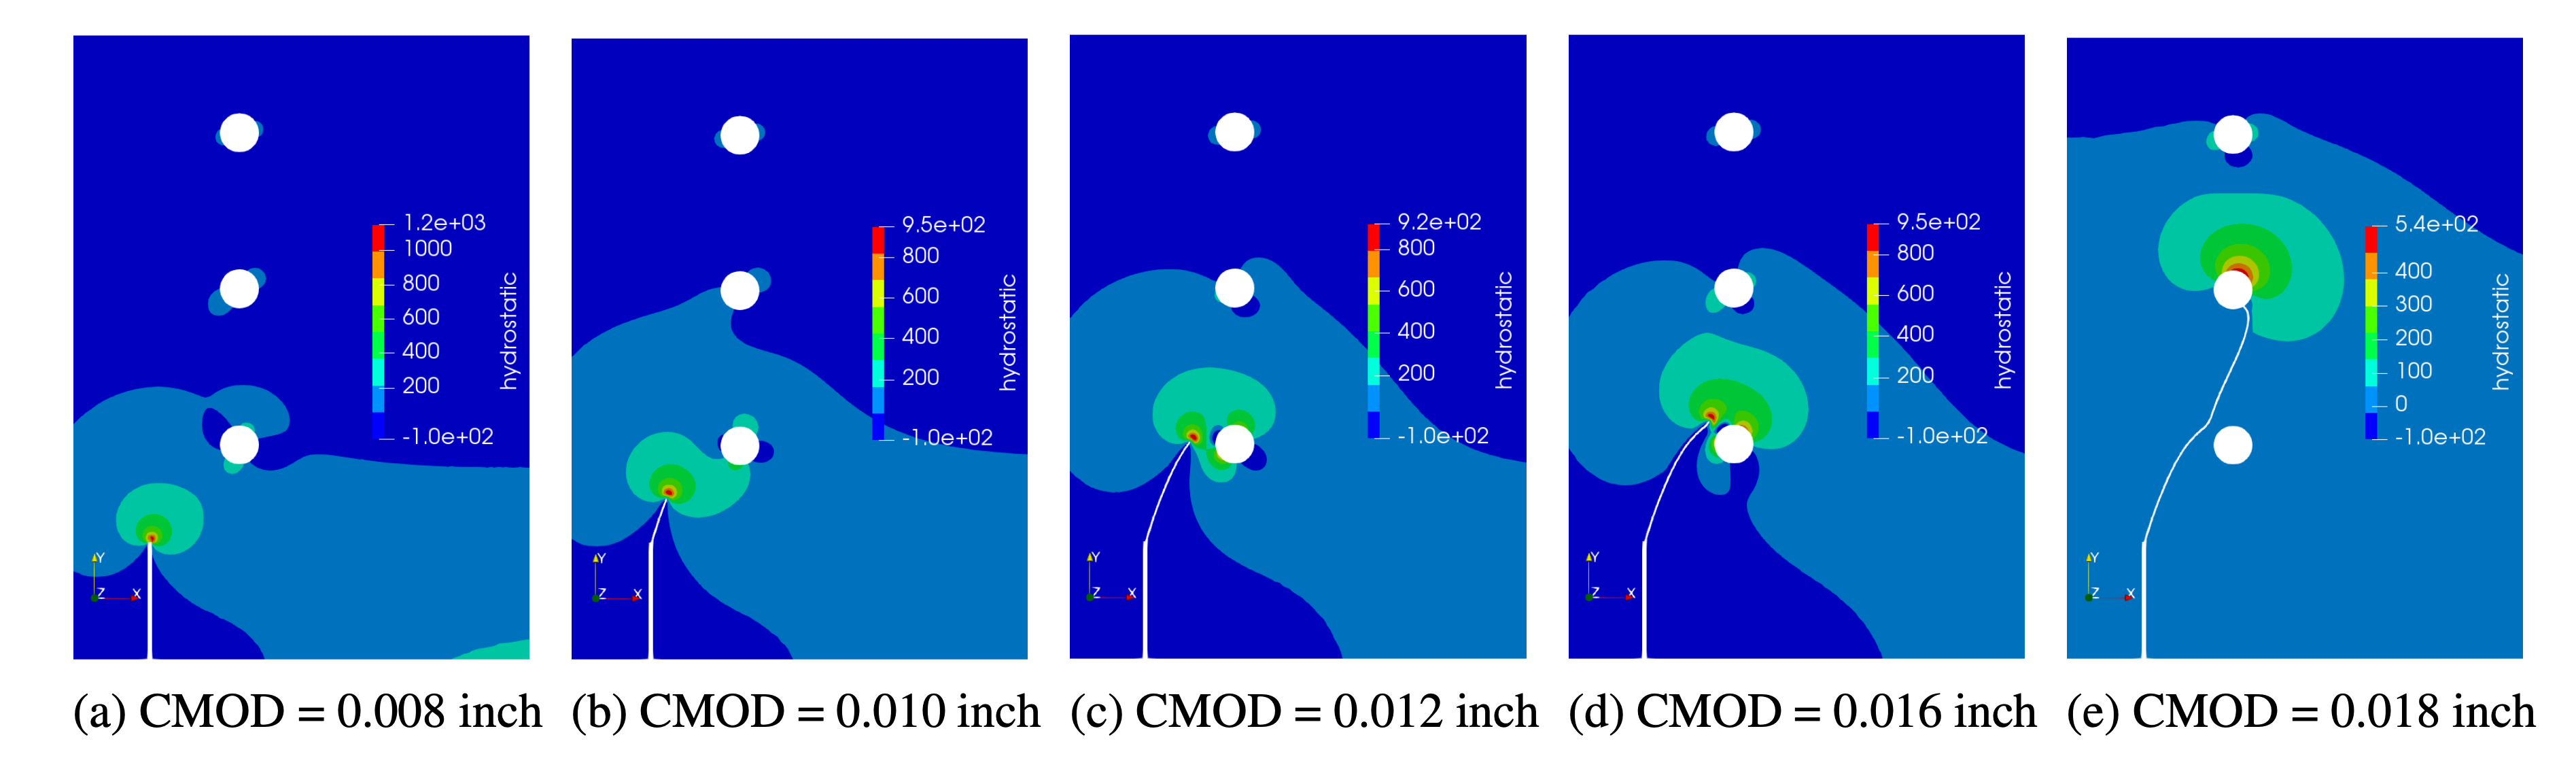
\includegraphics[width=0.9\textwidth]{figures1}
  \caption{Stacking multiple pictures together with sub-captions using the package \texttt{subfig}.}
  \label{fig:figures1}
\end{figure}

%---------------------------------------------------------------------------
\begin{figure*}[!h]
  \begin{snippetlatex}[caption={Stacking multiple images using \LaTeX\ package \texttt{subfig}.},label={snippet_sub_figures},framerule=1pt,tabsize=3]
    \begin{figure}[h!] \centering
    \subfloat[CMOD=0.008 inch]{\includegraphics[width=0.18\textwidth]{t14} \label{fig:a}}\;
    \subfloat[CMOD=0.010 inch]{\includegraphics[width=0.18\textwidth]{t16} \label{fig:b}}\;
    \subfloat[CMOD=0.012 inch]{\includegraphics[width=0.18\textwidth]{t20} \label{fig:c}}\;
    \subfloat[CMOD=0.016 inch]{\includegraphics[width=0.18\textwidth]{t28} \label{fig:d}}\;
    \subfloat[CMOD=0.018 inch]{\includegraphics[width=0.18\textwidth]{t30} \label{fig:e}}\;
    \caption{Asymmetric notched beam under three-point bending: crack evolution.}
    \label{fig:bittencourt-evolution}
    \end{figure}
  \end{snippetlatex}
\end{figure*}
%---------------------------------------------------------------------------

\begin{figure}[!h]
  \centering
  \subfloat[\texttt{Illustrator} and \texttt{LaTeXiT}]{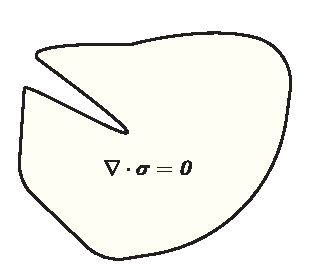
\includegraphics{Taylor-bar-setup}\label{fig:figures11a}}
  \subfloat[\texttt{Inkscape} and PDF\_TEX]{\input{Taylor-bar-setup_pdf_tex.pdf_tex}\label{fig:figures11b}}
  \caption{Using \texttt{Illustrator} and \texttt{Inskcape} to produce vector images with \LaTeX\ symbols. The font in figure (a) is slightly different from the one in the text ($\nabla\cdot\boldsymbol{\sigma} = \boldsymbol{\mathit{0}}$), while it matches perfectly in figure (b).}
  \label{fig:figures11}
\end{figure}

Another type of images in scientific papers is contour plots (see \cref{fig:figures1}), which are the outcomes of some visualization applications such as \texttt{ParaView}. We do not know how to match the font used in these images with the one in the text. We simply save them as PNG files and include them in the TEX document in the same manner as PDF images.

 Pay attention to the figure captions. Ideally, the reader should be able to ascertain the entire story just by reading the figure captions.

%--------------------------------------
\subsection{Tables}\label{sec:tabs}

Tables in scientific papers should be clear and focus on the data. Here are some suggestions for making good tables: avoid vertical lines, avoid double horizontal lines, avoid boxing up cells and leave enough space between rows. 
\cref{table:params} satisfies all the criteria. The \LaTeX\ code is shown in \cref{snippet_latex_table}.


 \begin{table}[h!]
      \centering
      \caption{Material parameters and characteristics for all simulations.}
      \setlength\fboxsep{0pt}
      \vskip-\topsep%
      \smallskip%
      \renewcommand\arraystretch{1.4}
      \colorbox{darkgray}{%
      \begin{tabularx}{0.7\textwidth}{lll}
      \toprule
      Parameter                & Section 5.1     & Section 5.2     \\
      \midrule
      Young's modulus [MPa]    & $210\times10^3$ & 145            \\
      Poisson's ratio [-]      & 0.3             & 0.45            \\
      Tensile strength [MPa]   & 2445            & 20              \\
          \midrule 
      Experimentally validated & n/a             & n/a            \\
      Solver                   & multi-step AM   & single-step AM implicit-explicit \\
      State                    & Plane strain    & Plane strain    \\
       \bottomrule
       \end{tabularx}%
      }
      \label{table:params}
      \end{table}


%---------------------------------------------------------------------------
\begin{figure*}[!h]
  \begin{snippetlatex}[caption={Typesetting tables in \LaTeX. Note that all columns are nicely aligned with \texttt{AlignTab} package in \texttt{Sublime Text}. There exist some softwares that can generate \texttt{Excel} tables to \LaTeX\ or visually generate \LaTeX\ tables online (\url{https://www.tablesgenerator.com}). },label={snippet_latex_table},framerule=1pt,tabsize=3]
      \begin{table}[h!]
      \centering
      \caption{Material parameters and characteristics for all simulations.}
      \setlength\fboxsep{0pt}
      \vskip-\topsep%
      \smallskip%
      \renewcommand\arraystretch{1.4}
      \colorbox{darkgray}{%      
      \begin{tabularx}{0.7\textwidth}{lll}
      \toprule
      Parameter                & Section 5.1     & Section 5.2     \\
      \midrule
      Young's modulus [MPa]    & $210\times10^3$ & 145            \\
      Poisson's ratio [-]      & 0.3             & 0.45            \\
      Tensile strength [MPa]   & 2445            & 20              \\
          \midrule 
      Experimentally validated & n/a             & n/a            \\
      Solver                   & multi-step AM   & single-step AM implicit-explicit \\
      State                    & Plane strain    & Plane strain    \\
       \bottomrule
       \end{tabularx}%
      }
      \label{table:params}
      \end{table}
  \end{snippetlatex}
\end{figure*}
%---------------------------------------------------------------------------

%The angle was \ang{12.3} The brightness was \SI{.23e7}{\candela} \SI{20}{MPa} \SI{10}{N.m.m^{-2}}


\subsection{Notations and equations}\label{sec:equation}

Avoid overly complex notations, see \cref{tab:complex-notation} for some examples. Try to introduce a nomenclature in the paper, to ease things for the reviewers and readers.  Sometimes, a table such as \cref{tab:notations} does a good job to introduce main notations. 

%%%%%%%%%%%%%%%%%%%%%%%%%%%%%%%%%%%%%%%%%%%%%%%%%%
\setlength{\fboxsep}{0pt}
\begin{table}[h!]
   \centering
     \setlength\fboxsep{0pt}
\vskip-\topsep%
\smallskip%
%\renewcommand\arraystretch{1.3}
\colorbox{darkgray}{%
   \begin{tabularx}{0.3\textwidth}{ll}
   \toprule
   Don't & Do  \\
  \midrule
   $\varkappa$ & $\kappa$  \\
   $\hbar$ & $\bar{h}$  \\
   $\underline{\underline{A}}$ & $\boldsymbol{A}$ or $A_{ij}$\\
  \bottomrule
 \end{tabularx}%
 }
\caption{Avoid overly complex notations.}
 \label{tab:complex-notation}
\end{table}

%%%%%%%%%%%%%%%%%%%%%%%%%%%%%%%%%%%%%%%%%%%%%%%%%%
\setlength{\fboxsep}{0pt}
\begin{table}[h!]
   \centering
     \setlength\fboxsep{0pt}
\vskip-\topsep%
\smallskip%
%\renewcommand\arraystretch{1.3}
\colorbox{darkgray}{%
   \begin{tabularx}{0.6\textwidth}{llX}
   \toprule
   Variable & Type  & Meaning\\
  \midrule
  $\mathbf{x}_p$ & Vector & Particle position (time-dependent)\\
  $\mathbf{X}_p$ & Vector & Particle initial position\\
  $m_p$ & Scalar & Particle mass\\
  $V_p$ & Scalar & Particle volume\\
  $\rho_p$ & Scalar & Particle density\\
  $T_p$ & Scalar & Particle temperature\\
  $\mathbf{P}_p$ & Tensor/Matrix & Particle 1$^\text{st}$ Piola-Kirchoff stress\\
  \bottomrule
 \end{tabularx}%
 }
\caption{Major notations can be put in a table.}
 \label{tab:notations}
\end{table}
%%%%%%%%%%%%%%%%%%%%%%%%%%%%%%%%%%%%%%%%%%%%%%%%%%

Ideally, the impact of scientific work should be determined by its scientific merit, rather than by presentational style. Unfortunately, \cite{Fawcett11735,Higginson_2016} showed that scientifically strong papers may have reduced impact if not presented in an accessible manner. 
The density of equations in an article in ecology and evolutionary biology has a significant negative impact on citation rates, with papers receiving 28\% fewer citations overall for each additional equation per page in the main text \citep{Fawcett11735}. For papers in physics, the number is 6\% fewer citations for each additional equation per page \citep{Higginson_2016}.

The lesson to learn from the above relation between the density of equations in a paper and its impact is to write less equations in the body of the paper. This can be achieved by removing unnecessary equations. If needed, some equations can be put in appendices.

%$\nicefrac{1}{2}$ ggglg;kgk, $\frac{1}{2}$ $\nicefrac{\alpha}{4\pi}$ $\frac{\alpha}{4\pi}$

%--------------------------------
\subsection{Two-column format}\label{sec:two-col}

Preparing two-column papers is harder than one-column papers. \cref{snippet_two_cols} presents \LaTeX\ snippets for long figures, tables and equations that span the whole width of the paper. That's all \LaTeX\ can do for you. For equations that are just a bit longer than one column, you have to manually modify them to make them fit.

%---------------------------------------------------------------------------
\begin{figure*}[!h]
  \begin{snippetlatex}[caption={Writing two-column papers using \LaTeX.},label={snippet_two_cols},framerule=1pt,tabsize=3]
    \usepackage{mathtools, cuted} % 2 colum format, long equation

     % big figure span the whole page
    \begin{figure*}[!h]
    \end{figure*}

    % big table span the whole page
    \begin{table*}[!h]
    \end{table*}
   
     % using strip for long equations
    \begin{strip}
     % put your long equation here
    \end{strip}
  \end{snippetlatex}
\end{figure*}
%---------------------------------------------------------------------------




%%%%%%%%%%%%%%%%%%%%%%%%%%%%%%%
\section{Submission}\label{sec:submission}

With the pressure to “publish” (or perish), it is increasingly difficult for students to resist the temptation to submit a “large” number of papers during their PhD. Some supervisors will also push the students to publish “too many” papers. 

Do not submit until you are really happy with the work, as it usually does not save time to submit a piece of work which we know ourselves could be improved: the reviewers will think likewise, or be even more critical than we are ourselves of our work. If on a final read of the paper you think: “Ah… I could have added this study. This argument is not completely convincing to me. This graph could be better plotted. I think I forgot some relevant literature. The notations are complex, perhaps the reader will have difficulties…” Then, do not submit immediately, improve your work, and submit it when it is ready. 

It is also useful to ask peers to read over your work. Before giving your first draft to your supervisor(s), have it proof-read by a peer (\textit{i.e.} if you are a PhD student, ask another PhD student for their opinion). This will bring the following positive points: 
It will value your peer as you think her/his opinion counts;
It will give you insights on how understandable your paper is by someone who is connected to your field but did not do exactly the same piece of research;
It will decrease the number of typos, which will enable your supervisor(s) to focus on the science as opposed to bumping over each spelling mistake, grammatical error, jargon.


%%%%%%%%%%%%%%%%%%%%%%%%%%%%%%%
\section{Conclusions}

Does this paper really need a conclusion section? Not really, but we are a bit conservative. So, here you are. Without claiming  originality of ideas presented in this short paper, we have presented a collection of  advices that can streamline the writing process. Following them would result in readable scientific articles which in turn save time for the authors,  the editors, the reviewers and the readers.


As \LaTeX\ and the tools we are relying on keep evolving, we will constantly update this article to reflect changes. The updated version of this paper and scripts can be obtained at the github account of the first author.

As with anything in this world, rules are there to be bent. Feel free to be creative as long as you write to inform not to impress. And happy writing.

%
%%%%%%%%%%%%%%%%%%%%%%%%%%%%%%%
\section*{Acknowledgments}

 The first author (V.P. Nguyen) thanks the funding support from the Australian Research Council via DECRA project DE160100577.  The third  author gratefully acknowledges the financial support of the Australian Research Council (ARC) Training Centre in Alloy Innovation for Mining Efficiency (IC160100036).

%% The Appendices part is started with the command \appendix;
%% appendix sections are then done as normal sections
%=============================================================================
\begin{appendix}
%=============================================================================
%\showthe\textwidth % => width of the pdf, see in log file, is 468 pt. use it in plot.py for great plots.
\section{Python script for plotting data}

This appendix present some \texttt{Python} scripts to produce high quality plots which have the same font used in the paper. One can use the script shown in \cref{snippet_matplotlib} to get PDFs or the one in \cref{snippet_matplotlib_pgf} to get PGF files. PGF pictures can be embedded as raw commands in LaTeX documents. The original source is \url{https://jwalton.info/Embed-Publication-Matplotlib-Latex/}.

The main idea is to get the correct figure size, and insert it in the paper without scaling. To determine the figure size, one first calculates the width of the paper, which can be done by inserting this command in the tex file:


\begin{verbatim}
\showthe\textwidth % => width of the pdf, see in log file, is 468 pt. 
\end{verbatim}
Then you can search for `width of the pdf' in this log file to find out the width of your paper.

\begin{figure*}[!h]
  \begin{snippet}[caption={Python script for plotting data.},label={snippet_matplotlib},framerule=1pt,tabsize=3]   
    import matplotlib as mpl
    import matplotlib.pyplot as plt

    def set_size(width, fraction=1, subplot=[1, 1]):
        if width == 'elsevier':
            width_pt = 468.
        elif width == 'beamer':
            width_pt = 307.28987
        else:
            width_pt = width
        fig_width_pt = width_pt * fraction      # Width of figure
        inches_per_pt = 1 / 72.27               # Convert from pt to inches
        golden_ratio = 0.75                     # (5**.5 - 1) / 2
        fig_width_in = fig_width_pt * inches_per_pt  # Figure width in inches
        fig_height_in = fig_width_in * golden_ratio * (subplot[0] / subplot[1])
        fig_dim = (fig_width_in, fig_height_in)
        return fig_dim

    parser = argparse.ArgumentParser(description='Plot the evolution of variables.',
                                     add_help=False,
                                     formatter_class=argparse.RawDescriptionHelpFormatter)


    parser.add_argument('--quiet', '-q', action='store_const', const=True, default=False,
                        help='do not show plot.')
    args = parser.parse_args()

    # Using seaborn's style
    plt.style.use('seaborn-colorblind')  

    nice_fonts = {
            "text.usetex": True,
            "font.family": "serif",
            "axes.labelsize": 10,
            "font.size": 10,
            "legend.fontsize": 8,
            "xtick.labelsize": 8,
            "ytick.labelsize": 8,
    }

    mpl.rcParams.update(nice_fonts)

    # Dimer 5: Read Data
    fnames = ['log.mpm', 'dam-break-Sun.csv', 'water-break-experiment.csv']
    dat    = [pylab.genfromtxt(f,skip_header=1) for f in fnames]

    fig, ax = plt.subplots(1, 1, figsize=set_size('elsevier', fraction=0.6))
    # fig, (ax1,ax2) = plt.subplots(1, 2, figsize=set_size(width, subplot=[1, 2]))

    for i, f in enumerate(fnames):   
        x = dat[i][:,3]
        y = dat[i][:,4]
        ax.plot(x, y, color='black', label='MPM',linewidth=1.5, linestyle='dotted')
       
        xmax = max(xmax, np.max(x))
        ymax = max(ymax, np.max(y))
         
    ax.set_xlabel(r'$T$')
    ax.set_ylabel(r'$L(T)$')
    ax.set_ylim(1.0, 2.8)
    ax.set_xlim(0, 1.6)
    ax.legend(loc=0)
    plt.tight_layout()
    plt.savefig('./water-break-plot.pdf', format='pdf', bbox_inches='tight')

    if args.quiet == False:
        plt.show()
  \end{snippet}
\end{figure*}

\begin{figure*}[!h]
  \begin{snippet}[caption={Python script for plotting data.},label={snippet_matplotlib_pgf},framerule=1pt,tabsize=3]   
    nice_fonts = {
            "text.usetex": True,
            "font.family": "serif",
            "pgf.texsystem": "pdflatex",
            "font.family": "serif",
            "font.serif": [],
            "font.sans-serif": [],
            "font.monospace": [],
            "pgf.preamble": [
            # put LaTeX preamble declarations here
            r"\usepackage[utf8x]{inputenc}",
            r"\usepackage[T1]{fontenc}",
            # macros defined here will be available in plots, e.g.:
            r"\newcommand{\vect}[1]{#1}",
            # You can use dummy implementations, since you LaTeX document
            # will render these properly, anyway.
            ],
            "axes.labelsize": 10,
            "font.size": 10,
            "legend.fontsize": 8,
            "xtick.labelsize": 8,
            "ytick.labelsize": 8,
    }
    plt.savefig('./cold-spray-plots.pgf', bbox_inches='tight') 
    if args.quiet == False:
        plt.show()
  \end{snippet}
\end{figure*}

\begin{rmk}
If you are using \texttt{Matlab}, then try this script \texttt{matlab2tikz} for converting \texttt{Matlab} figures into native TikZ/Pgfplots figures. The script can be found at
\url{https://www.mathworks.com/matlabcentral/fileexchange/22022-matlab2tikz-matlab2tikz}.
\end{rmk}



\end{appendix}


%%%%%%%%%%%%%%%%%%%%%%%%
\section*{References}


% %%%%%%% BIB files (bibtex)
%\bibliographystyle{plainnat}
\bibliographystyle{abbrvnat} % => just V. P. Nguyen, not Phu Nguyen, ...
%\bibliographystyle{natbib}
\bibliography{writing}

% if biblatex is used
%\printbibliography

\end{document}
